% Choose the language of your thesis passing 'french' or 'english' as
% \documentclass option.
% Note1: The 'page de garde' will always be written in French.
% Note2: You will have an error if you change the language of the document and
%        compile it without cleaning the auxiliary files. Compiling it again
%        should solve the problem.
\documentclass[english,a4paper,11pt,twoside]{StyleThese}
\newcommand{\included}{}
\usepackage{pdfpages}

\usepackage{amsmath,amssymb}             % AMS Math
\usepackage[T1]{fontenc}
\usepackage[utf8x]{inputenc}
\usepackage{babel}
\usepackage{datetime}

\usepackage{array}
% \newcolumntype{x}[1]{>{\centering\arraybackslash\hspace{0pt}}p{#1}}
\newcolumntype{x}[1]{>{\centering\let\newline\\\arraybackslash\hspace{0pt}}p{#1}}

\usepackage{lmodern}
\usepackage{tabularx}
%\usepackage{tabular}
\usepackage{multirow}
\usepackage{enumitem}
\usepackage{subcaption}
\usepackage{siunitx}
% \usepackage{algorithm}
\usepackage{algpseudocode}
\usepackage{hhline}
\usepackage[left=1.2in,right=1.0in,top=1.1in,bottom=1.1in,includefoot,includehead,headheight=13.6pt]{geometry}
\renewcommand{\baselinestretch}{1.05}
% Table of contents for each chapter

\usepackage[nottoc, notlof, notlot]{tocbibind}
\usepackage{minitoc}
\setcounter{minitocdepth}{2}
\mtcindent=15pt
% Use \minitoc where to put a table of contents

\usepackage{aecompl}

% Glossary / list of abbreviations

\usepackage[intoc]{nomencl}
\iftoggle{ThesisInEnglish}{%
\renewcommand{\nomname}{Glossary}
}{ %
\renewcommand{\nomname}{Liste des Abréviations}
}

\makenomenclature

% My pdf code

\usepackage{ifpdf}

\ifpdf
  \usepackage{graphicx}
  \usepackage[a4paper,pagebackref,hyperindex=true]{hyperref}
  \usepackage{tikz}
  \usetikzlibrary{arrows,shapes,calc}
\else
  \usepackage{graphicx}
  \DeclareGraphicsExtensions{.ps,.eps}
  \usepackage[a4paper,dvipdfm,pagebackref,hyperindex=true]{hyperref}
\fi

\graphicspath{{.}{images/}}

%% nicer backref links. NOTE: The flag ThesisInEnglish is used to define the
% language in the back references. Read more about it in These.tex

\iftoggle{ThesisInEnglish}{%
\renewcommand*{\backref}[1]{}
\renewcommand*{\backrefalt}[4]{%
\ifcase #1 %
(Not cited.)%
\or
(Cited in page~#2.)%
\else
(Cited in pages~#2.)%
\fi}
\renewcommand*{\backrefsep}{, }
\renewcommand*{\backreftwosep}{ and~}
\renewcommand*{\backreflastsep}{ and~}
}{%
\renewcommand*{\backref}[1]{}
\renewcommand*{\backrefalt}[4]{%
\ifcase #1 %
(Non cité.)%
\or
(Cité en page~#2.)%
\else
(Cité en pages~#2.)%
\fi}
\renewcommand*{\backrefsep}{, }
\renewcommand*{\backreftwosep}{ et~}
\renewcommand*{\backreflastsep}{ et~}
}

% Links in pdf
\usepackage{color}
\definecolor{linkcol}{rgb}{0,0,0.4} 
\definecolor{citecol}{rgb}{0.5,0,0} 
\definecolor{linkcol}{rgb}{0,0,0} 
\definecolor{citecol}{rgb}{0,0,0}
% Change this to change the informations included in the pdf file

\hypersetup
{
bookmarksopen=true,
pdftitle=Human-Aware Robot Task Planning: Theory of Mind and Anticipation of Human Decisions and Actions,
pdfauthor=Anthony Favier, %auteur du document
pdfsubject=Thesis, %sujet du document
%pdftoolbar=false, %barre d'outils non visible
pdfmenubar=true, %barre de menu visible
pdfhighlight=/O, %effet d'un clic sur un lien hypertexte
colorlinks=true, %couleurs sur les liens hypertextes
pdfpagemode=None, %aucun mode de page
pdfpagelayout=SinglePage, %ouverture en simple page
pdffitwindow=true, %pages ouvertes entierement dans toute la fenetre
linkcolor=linkcol, %couleur des liens hypertextes internes
citecolor=citecol, %couleur des liens pour les citations
urlcolor=linkcol %couleur des liens pour les url
}

% definitions.
% -------------------

\setcounter{secnumdepth}{3}
\setcounter{tocdepth}{2}

% Some useful commands and shortcut for maths:  partial derivative and stuff

\newcommand{\pd}[2]{\frac{\partial #1}{\partial #2}}
\def\abs{\operatorname{abs}}
\def\argmax{\operatornamewithlimits{arg\,max}}
\def\argmin{\operatornamewithlimits{arg\,min}}
\def\diag{\operatorname{Diag}}
\newcommand{\eqRef}[1]{(\ref{#1})}

\usepackage[figuresleft]{rotating}                    % Sideways of figures & tables
%\usepackage{bibunits}
%\usepackage[sectionbib]{chapterbib}          % Cross-reference package (Natural BiB)
%\usepackage{natbib}                  % Put References at the end of each chapter
                                         % Do not put 'sectionbib' option here.
                                         % Sectionbib option in 'natbib' will do.


% \usepackage{txfonts}                     % Public Times New Roman text & math font
% \usepackage[ED=MITT-InfoTel, Ets=UT3]{tlsflyleaf}
\usepackage{fancyhdr}                    % Fancy Header and Footer  
%%% Fancy Header %%%%%%%%%%%%%%%%%%%%%%%%%%%%%%%%%%%%%%%%%%%%%%%%%%%%%%%%%%%%%%%%%%
% Fancy Header Style Options

\pagestyle{fancy}                       % Sets fancy header and footer
\fancyfoot{}                            % Delete current footer settings

%\renewcommand{\chaptermark}[1]{         % Lower Case Chapter marker style
%  \markboth{\chaptername\ \thechapter.\ #1}}{}} %

%\renewcommand{\sectionmark}[1]{         % Lower case Section marker style
%  \markright{\thesection.\ #1}}         %

\fancyhf{}
\fancyhead[LE,RO]{\bfseries\thepage}    % Page number (boldface) in left on even
% pages and right on odd pages
% \renewcommand{\chaptermark}[1]{\markboth{\nouppercase{\thechapter.\ #1}}{}}
\fancyhead[RE]{\bfseries\nouppercase{\leftmark}}      % Chapter in the right on even pages
\fancyhead[LO]{\bfseries\nouppercase{\rightmark}}     % Section in the left on odd pages

\let\headruleORIG\headrule
\renewcommand{\headrule}{\color{black} \headruleORIG}
\renewcommand{\headrulewidth}{1.0pt}
\usepackage{colortbl}
\arrayrulecolor{black}

\fancypagestyle{plain}{
  \fancyhead{}
  \fancyfoot{}
  \renewcommand{\headrulewidth}{0pt}
}

%\usepackage{MyAlgorithm}
%\usepackage[noend]{MyAlgorithmic}

%%% Clear Header %%%%%%%%%%%%%%%%%%%%%%%%%%%%%%%%%%%%%%%%%%%%%%%%%%%%%%%%%%%%%%%%%%
% Clear Header Style on the Last Empty Odd pages
\makeatletter

\def\cleardoublepage{\clearpage\if@twoside \ifodd\c@page\else%
  \hbox{}%
  \thispagestyle{empty}%              % Empty header styles
  \newpage%
  \if@twocolumn\hbox{}\newpage\fi\fi\fi}

\makeatother
 
%%%%%%%%%%%%%%%%%%%%%%%%%%%%%%%%%%%%%%%%%%%%%%%%%%%%%%%%%%%%%%%%%%%%%%%%%%%%%%% 
% Prints your review date and 'Draft Version' (From Josullvn, CS, CMU)
\newcommand{\reviewtimetoday}[2]{\special{!userdict begin
    /bop-hook{gsave 20 710 translate 45 rotate 0.8 setgray
      /Times-Roman findfont 12 scalefont setfont 0 0   moveto (#1) show
      0 -12 moveto (#2) show grestore}def end}}
% You can turn on or off this option.
% \reviewtimetoday{\today}{Draft Version}
%%%%%%%%%%%%%%%%%%%%%%%%%%%%%%%%%%%%%%%%%%%%%%%%%%%%%%%%%%%%%%%%%%%%%%%%%%%%%%% 

\newenvironment{maxime}[1]
{
\vspace*{0cm}
\hfill
\begin{minipage}{0.5\textwidth}%
%\rule[0.5ex]{\textwidth}{0.1mm}\\%
\hrulefill $\:$ {\bf #1}\\
%\vspace*{-0.25cm}
\it 
}%
{%

\hrulefill
\vspace*{0.5cm}%
\end{minipage}
}

\let\minitocORIG\minitoc
\renewcommand{\minitoc}{\minitocORIG \vspace{1.5em}}

\usepackage{multirow}
%\usepackage{slashbox}

\newenvironment{bulletList}%
{ \begin{list}%
	{$\bullet$}%
	{\setlength{\labelwidth}{25pt}%
	 \setlength{\leftmargin}{30pt}%
	 \setlength{\itemsep}{\parsep}}}%
{ \end{list} }

\newtheorem{definition}{Definition}
\renewcommand{\epsilon}{\varepsilon}

% centered page environment

\newenvironment{vcenterpage}
{\newpage\vspace*{\fill}\thispagestyle{empty}\renewcommand{\headrulewidth}{0pt}}
{\vspace*{\fill}}

\usepackage{tablefootnote}

\newcommand{\mysection}[1]{%
    \section*{#1}%
    \addcontentsline{toc}{section}{#1}%
    \markright{#1}%
}
\usepackage[disable,colorinlistoftodos,prependcaption,textsize=tiny]{todonotes}
\usepackage{xargs}   % Use more than one optional parameter in a new commands
\usepackage{xcolor}  % Coloured text
\usepackage{xspace}

\usepackage{hyperref}
\usepackage{amsmath}
\usepackage{amssymb}
\usepackage{bbm}
%\usepackage{mathbbol}

\usepackage{longtable}

\usepackage{booktabs}
\usepackage{courier}

\usepackage{moreverb}

% \usepackage[bottom]{footmisc}
\definecolor{lightgray}{gray}{0.5}

\usepackage{listings}
\usepackage[normalem]{ulem}
\useunder{\uline}{\ul}{}

\newtheorem{theorem}{Theorem}

\usepackage{algorithm}
% \usepackage[noend]{algpseudocode} 
% limit indentation in algorithms
% \algrenewcommand\algorithmicindent{1.0em}%
% \algnewcommand{\IIf}[1]{\State\algorithmicif\ #1\ \algorithmicthen}
% \algnewcommand{\EndIIf}{\unskip\ \algorithmicend\ \algorithmicif}

\newcommand*{\field}[1]{\mathbb{#1}}%

%%%%%%%%%%%%%%%%%%%%%%%%
%	 listing formats   %
%%%%%%%%%%%%%%%%%%%%%%%%

\lstdefinestyle{HatpPlan}{
  language=C,
  commentstyle=\itshape\color{green!25!black},
}

\lstdefinestyle{OwlTurtle}{
  language=C,
  keywordstyle=\bfseries\color{darkgray},
  morekeywords={rdf:type, rdfs:domain, rdfs:subPropertyOf, rdfs:range, :hasSubtask, :DecompositionUsedBy, rdfs:subClassOf, :hasDecomposition, owl:inverseOf},
  alsoletter=:
}

\lstdefinestyle{OwlTurtle_indiv}{
  language=C,
  keywordstyle=\bfseries\color{darkgray},
  morekeywords={rdf, rdfs, type, domain, subPropertyOf, range, hasSubtask, DecompositionUsedBy, subClassOf, hasDecomposition, Cut_hasParameter, A, V, K, hasColor, hasCadModel, isOn, isInRegion, isAtEndOfPath, isAtLeftOfPath, hasAtRight, isInFrontOf, objectActedOn, eventOccursAt, startTime}
}

\lstdefinestyle{Labels}{
  language=C,
  basicstyle = \fontencoding{T1}\ttfamily \color{black} \footnotesize
}

%%%%%%%%%%%%%%%%%%%%%%%%%%%%%%%%%%%%%%%%%%%%%%%%%%%%%%%%%%
%                         NEW                            %
%%%%%%%%%%%%%%%%%%%%%%%%%%%%%%%%%%%%%%%%%%%%%%%%%%%%%%%%%%

\newcommandx{\chapabstract}[1]{\textbf{\textit{#1}}}


\newcommandx{\agent}{\varphi}
\newcommandx{\agentstate}[2][1,2,usedefault=]{\sigma^{#1}_{#2}}
\newcommandx{\agentmodel}[1][1,usedefault=]{\mathcal{M}^{#1}}
\newcommandx{\agenda}[2][1,2,usedefault=]{d^{#1}_{#2}}
\newcommandx{\partialplan}[2][1,2,usedefault=]{\pi^{#1}_{#2}}
\newcommandx{\valf}[2][1,2,usedefault=]{val^{#1}_{#2}}
\newcommandx{\obsf}[1][1,usedefault=]{obs_{#1}}
\newcommandx{\locf}[1][1,usedefault=]{loc_{#1}}
\newcommandx{\observable}{\texttt{OBS}}
\newcommandx{\inferable}{\texttt{INF}}




%%%%%%%%%%%%%%%%%%%%%%%%%%%%%%%%%%%%%%%%%%%%%%%%%%%%%%%%%%
%                         OLD                            %
%%%%%%%%%%%%%%%%%%%%%%%%%%%%%%%%%%%%%%%%%%%%%%%%%%%%%%%%%%

%%%%%%%%%%%%%%%%%%%%%%%%
%	  TODO commands    %
%%%%%%%%%%%%%%%%%%%%%%%%

\setlength{\marginparwidth}{3cm}
\newcommandx{\unsure}[2][1=]{\todo[linecolor=red,backgroundcolor=red!25,bordercolor=red,#1]{#2}}
\newcommandx{\change}[2][1=]{\todo[linecolor=blue,backgroundcolor=blue!25,bordercolor=blue,#1]{#2}}
\newcommandx{\info}[2][1=]{\todo[linecolor=olive,backgroundcolor=olive!25,bordercolor=olive,#1]{#2}}
\newcommandx{\improvement}[2][1=]{\todo[linecolor=violet,backgroundcolor=violet!25,bordercolor=violet,#1]{#2}}
\newcommandx{\thiswillnotshow}[2][1=]{\todo[disable,#1]{#2}}

%%%%%%%%%%%%%%%%%%%%%%%%
%	Knowledge bases    %
%%%%%%%%%%%%%%%%%%%%%%%%

\newcommand \kb{K}

% Ontology definition

\newcommand \kbs{\kb_S}
\newcommand \Abox{\mathbb{A}}
\newcommand \Tbox{\mathbb{T}}
\newcommand \Rbox{\mathbb{R}}

\newcommand \propset{P}
\newcommand \classset{T}
\newcommand \indivset{A}
\newcommand \relationset{R}
\newcommand \annotationset{E}

\newcommand \domainset{Dom}
\newcommand \rangeset{Ran}
\newcommand \inclset{Incl}
\newcommand \invset{Inv}
\newcommand \inheritset{C}

\newcommand \indiv{a}
\newcommand \class{t}

\newcommand \labelfunc {\mathcal{L}}
\newcommand \alabel{\mathcal{L}_a}
\newcommand \tlabel{\mathcal{L}_t}
\newcommand \plabel{\mathcal{L}_p}
\newcommand \alabelag[1]{\mathcal{L}_{a#1}}
\newcommand \tlabelag[1]{\mathcal{L}_{t#1}}
\newcommand \plabelag[1]{\mathcal{L}_{p#1}}

\newcommand \subject{s}
\newcommand \property{p}
\newcommand \object{o}
\newcommand \relation{r}

\newcommand{\sparql}{\textsc{sparql}}

% Timeline definition

\newcommand \kbe{\kb_E}
\newcommand \tinterval{\mathcal{T}}
\newcommand \tstart{\tau_s}
\newcommand \tend{\tau_e}
\newcommand \taction{\alpha}

%%%%%%%%%%%%%%%%%%%%%%%%
%	      REG          %
%%%%%%%%%%%%%%%%%%%%%%%%

\newcommand \goalindiv{\indiv_t}
\newcommand \usablepropset{U}
\newcommand \problem{\mathcal{P}}
\newcommand \solution{\mathcal{S}}

\newcommand \costfunc{\mathcal{C}}
\newcommand \varset{X}
\newcommand \var{x}

\newcommand \cost{\mathbbm{c}}
\newcommand \node{\mathbbm{n}}
\newcommand \state{\mathbbm{s}}
\newcommand \action{\mathbbm{a}}

\newcommand \softdiff{\,\delta\,}
\newcommand \harddiff{\,\Delta\,}

\newcommand \symboltable{\mathcal{S}}
\newcommand \matchtable{\mathcal{M}}

\newcommand \us{$\mu$s\xspace}

\newcommand{\tovariable}{\textsc{ToVariable}}
\newcommand{\toquery}{\textsc{ToQuery}}
\newcommand{\sparqlresult}{\textsc{SparqlResult}}
\newcommand{\createchild}{\textsc{CreateChild}}
\newcommand{\actions}{\textsc{Actions}}
\newcommand{\goaltest}{\textsc{GoalTest}}
\newcommand{\typingactions}{\textsc{TypingActions}}
\newcommand{\differenceactions}{\textsc{DifferentiationActions}}

\newcommand{\additions}{\textsc{CreateAddition}}
\newcommand{\typingadditions}{\textsc{TypingAdditions}}
\newcommand{\differenceadditions}{\textsc{DifferentiationAdditions}}
\newcommand{\actingadditions}{\textsc{ActingAdditions}}
\newcommand{\completionadditions}{\textsc{CompletionAdditions}}
\newcommand{\compoundadditions}{\textsc{CompoundAdditions}}
\newcommand{\createtree}{\textsc{CreateTree}}
\newcommand{\getsubtrees}{\textsc{getSubTrees}}

%%%%%%%%%%%%%%%%%%%%%%%%
%	      HTN          %
%%%%%%%%%%%%%%%%%%%%%%%%

\newcommand \tasknetwork{N}
\newcommand \task{n}
\newcommand \primtaskset{Pt}
\newcommand \abstaskset{At}
\newcommand \decomposet{D}
\newcommand \decompo{d}
\newcommand \abstracttask{\upsilon}
\newcommand \HTN{Pl}
\usepackage[acronym]{glossaries}

\makenoidxglossaries

\newacronym{ai}{AI}{Artificial Intelligence}
\newacronym{hhi}{HHI}{Human-Human Interaction}
\newacronym{hci}{HCI}{Human-Computer Interaction}
\newacronym{hri}{HRI}{Human-Robot Interaction}
\newacronym{hrc}{HRC}{Human-Robot Collaboration}
\newacronym{han}{HAN}{Human-Aware Navigation}
\newacronym{cohan}{CoHAN}{Cooperative Human-Aware Navigation}
\newacronym{orca}{ORCA}{Optimal Reciprocal Collision Avoidance}
\newacronym{sfm}{SFM}{Social Force Model}
\newacronym{pomdp}{POMDP}{Partially Observable Markov Decision Process}
\newacronym{mdp}{MDP}{Markov Decision Process}
\newacronym{amm}{AMM}{Agent Markov Model}
\newacronym{ros}{ROS}{Robot Operating System}
\newacronym{hatpehda}{HATP/EHDA}{Human-Aware Task Planner Emulating Human Decisions and Actions}
\newacronym{hatp}{HATP}{Hierarchical Agent-based Task Planner}
\newacronym{tom}{ToM}{Theory of Mind}
\newacronym{htn}{HTN}{Hierarchical Task Network}
\newacronym{inhus}{InHuS}{Intelligent Human Simuator}
\newacronym{imhus}{IMHuS}{Intelligent Multi Human Simuator}
\newacronym{sa}{SA}{Situation Assessment}
\newacronym{del}{DEL}{Dynamic Epistemic Logic}
\newacronym{id}{ID}{Identification}
\newacronym{dag}{DAG}{Directed Acyclic Graph}


\setlength{\belowcaptionskip}{-6pt}

%%%%%%%%%%%%%%% Uncomment this to generate new Cover page%%%%%%%%%
\usepackage[ED=MITT-InfoTel, Ets=INP]{tlsflyleaf}
%% This is file `example.tex',
%% Copyright 2013 Tristan GREGOIRE
%% Copyright 2015 Yann BACHY
%
% This work may be distributed and/or modified under the
% conditions of the LaTeX Project Public License, either version 1.3
% of this license or (at your option) any later version.
% The latest version of this license is in
%   http://www.latex-project.org/lppl.txt
% and version 1.3 or later is part of all distributions of LaTeX
% version 2005/12/01 or later.
%
%
% This work has the LPPL maintenance status `maintained'.
% 
% The Current Maintainer of this work is T. GREGOIRE
%

%\documentclass{book}

% Loading the tlsflyleaf.sty package require some option to define the
% establishment name, the doctoral school and the PhD speciality.
% In that aim you have 2 key-value option:
%   - Ets=<value> : define the establishment name
%   - ED=<value>  : define the doctoral school and speciality
%   - ED2=<value> : define the second speciality ("double mention"). OPTIONAL.
% The full list of accepted values for each option could be find either
% in the documentation or in ED-list.txt and Ets-list.txt files provide with the package.
%\usepackage[ED=MITT - STICRT, Ets=INSA]{tlsflyleaf}
%\usepackage[ED=SDU2E-Ast, ED2=SDU2E-Eco, Ets=UT3]{tlsflyleaf}
%\usepackage[ED=MITT - STICRT, Ets=UT3]{tlsflyleaf}

% ==================
% Setup basic string
% - PhD Title
% - author
% - defence date
% - laboratory
% - cotutelle
\title{\textbf{\large Human-Aware Robot Task Planning:\\Theory of Mind and Anticipation of Human Decisions and Actions}}
% \title{\textbf{\large Planification de Tâches pour un Robot Collaboratif :\\Théorie de l'Esprit et Anticipation des Décisions et Actions de l'Humain}}
\author{Anthony Favier}
\defencedate{30/04/2024}
\lab{Laboratoire d'Analyse et d'Architecture des Systèmes (LAAS-CNRS)}
%\cotutelle{}

% ==================
% Setup people like your boss, the jury team and the referees
% - First you need to define how number they will be in each category
%   It is done with the commands \nboss{n}, \nreferee{n} and \njudge{n}.
%   You can define more people in each category than the number given 
%   but only the first "\npeople" will be print.
% - Then use the command \makesomeone{<category>}{<number>}{<name>}{<status>}{<other>}
%   where:
%     <category> should be select in ['boss', 'referee', 'judge']
%     <number>   is the rank for printing the person. 
%                Only number <= "\npeople" will be printed
%     <name>     First name and las name of the people
%     <status>   Is (s)he a "charg\'e de recher" ou un "professeur d'universit\'e"...
%     <other>    What ever string you want to add (laboratory, jury member place...).
%% Boss
\nboss{1}
\makesomeone{boss}{1}{Rachid ALAMI}{}{} % Sera afiche en premier
%% Referee
\nreferee{2}
\makesomeone{referee}{1}{Mohamed CHETOUANI}{}{}
\makesomeone{referee}{2}{Julie SHAH}{}{}
%% Jury
\njudge{7}
\makesomeone{judge}{1}{Mohamed CHETOUANI}{Professeur}{Rapporteur}
\makesomeone{judge}{2}{Julie SHAH}{Professeure}{Rapporteur}
\makesomeone{judge}{3}{Jean-Charles FABRE}{Professeur}{Membre du Jury}
\makesomeone{judge}{4}{Luca IOCCHI}{Professeur}{Membre du Jury}
\makesomeone{judge}{5}{Simon LACROIX}{Directeur de Recherche}{Membre du Jury}
\makesomeone{judge}{6}{Catherine PELACHAUD}{Directrice de Recherche}{Membre du Jury}
\makesomeone{judge}{7}{Rachid ALAMI}{Directeur de Recherche}{Directeur de Thèse}

% ============================================================
% DOCUMENT
% \begin{document}
%   \makeflyleaf
% \end{document}

%%%%%%%%%%%%%%% Uncomment this to generate new Cover page%%%%%%%%%

\sloppy
\begin{document}

%%%%%%%%%%%%%%% Uncomment this to generate new Cover page %%%%%%%%%
\makeflyleaf
%%%%%%%%%%%%%%% Uncomment this to generate new Cover page %%%%%%%%%

%%%%%%%%%%%%%%% Uncomment this to use custom Cover page %%%%%%%%%
% 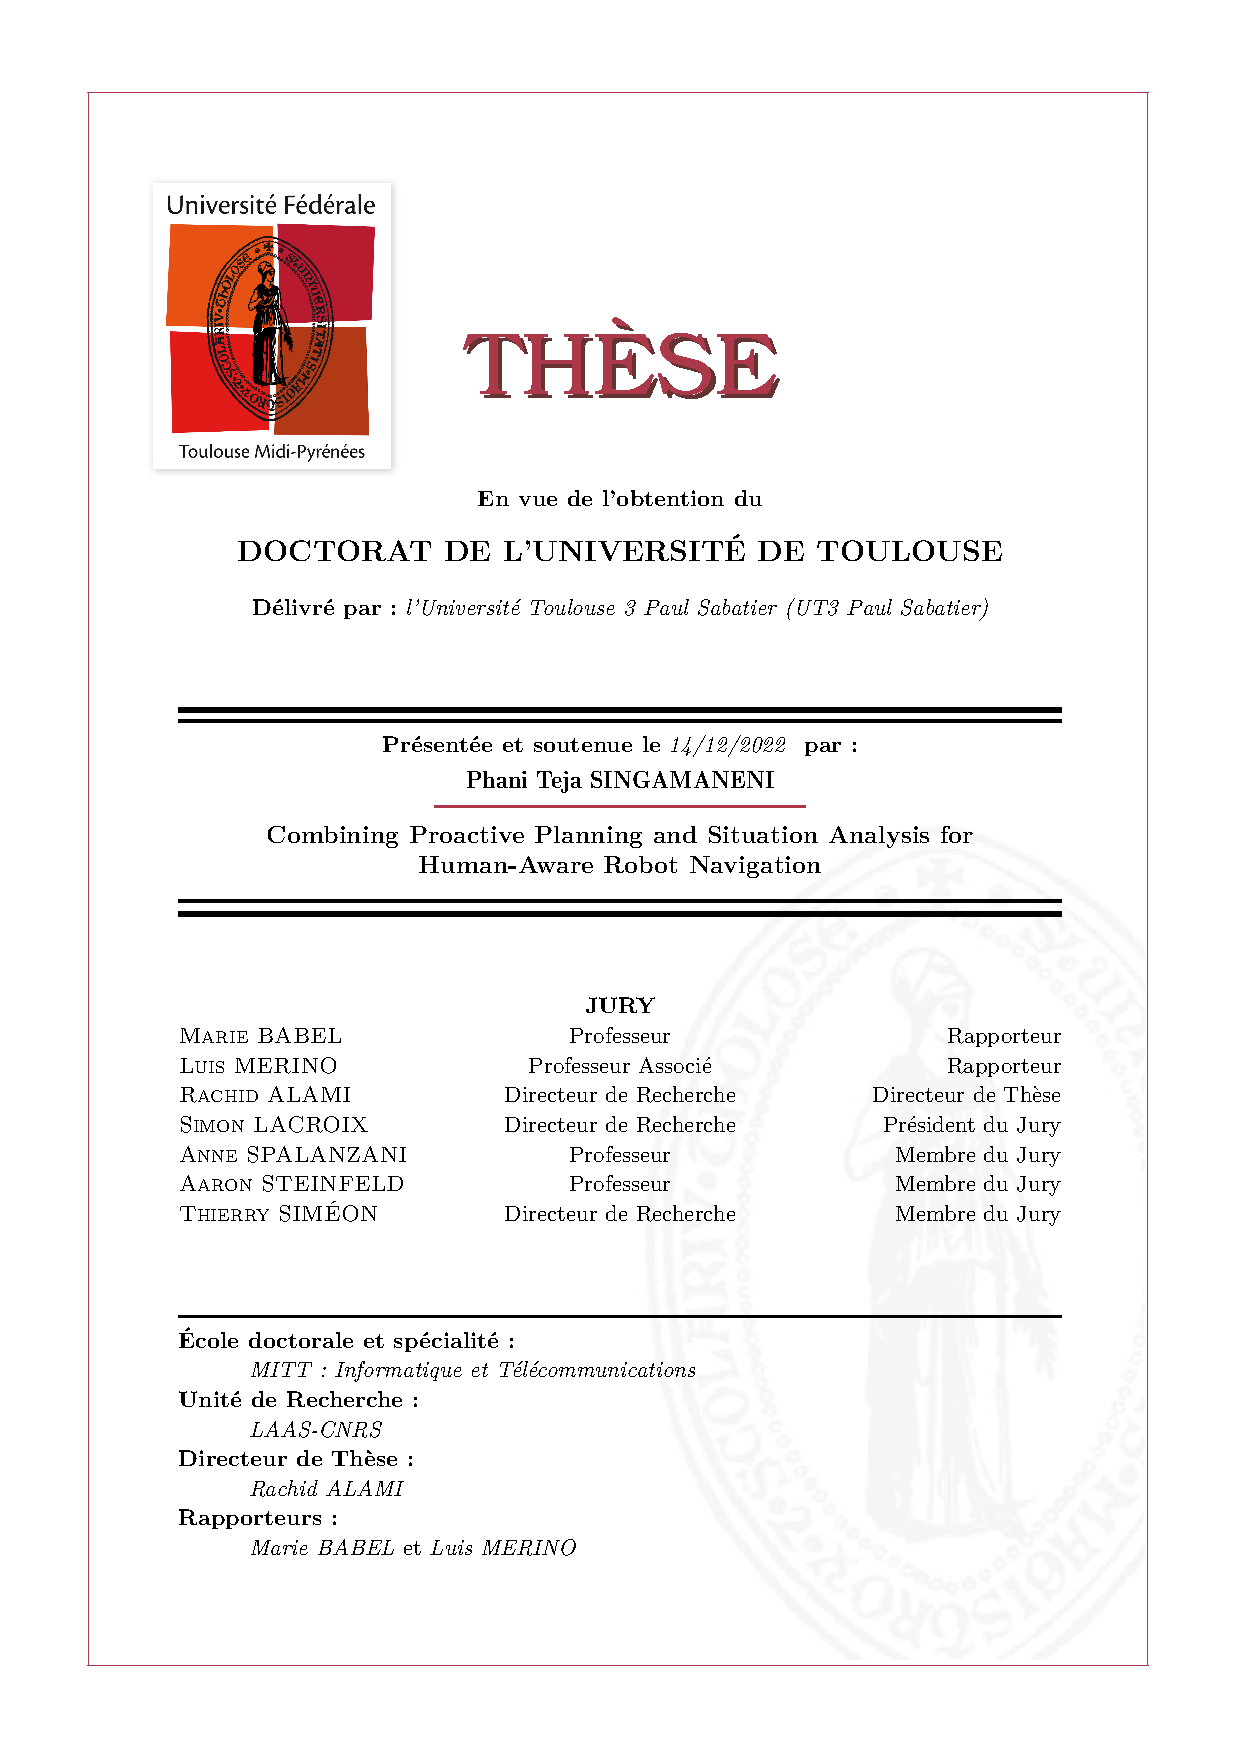
\includepdf[pages=-]{custom_cover_new.pdf}
%%%%%%%%%%%%%%% Uncomment this to use custom Cover page %%%%%%%%%


\cleardoublepage

\dominitoc

\pagenumbering{roman}

\cleardoublepage

%%%% Acknowledgments %%%%%
%%% Needs an update before and after the defence, write last
% \section*{Remerciemments}
 
blabla 

%%%% Abstract %%%%%
% \chapter*{Abstract}

% 4000 caractères

Although human-robot collaboration can be beneficial, most of today's robots work in spaces physically separated from humans, or their capabilities are severely limited in close proximity to humans. This work aims to bridge the gap between robotic capabilities and human expectations, fostering a new era of seamless and intuitive collaboration between humans and robots in shared environments to perform industrial, service or domestic tasks. More specifically, this manuscript presents a study of decision-making in the context of human-robot collaboration, particularly in the areas of task planning and simulating intelligent agents.

First, we discuss various fields and works related to human-robot collaboration to better understand my work's context. After an introduction to the HATP/EHDA task planner, I present my first contribution, which incorporates some concepts from the Theory Of Mind into task planning. Some models and algorithms are proposed and evaluated to better estimate and maintain human knowledge during collaboration, in order to better anticipate human behavior. As a result, we can identify when humans have false beliefs about a fact that is evaluated as relevant to the task. In this case, the robot can proactively inform the humans to correct the false information, or the robot can deliberately delay its actions so that the humans can see them. Our results show that this scheme effectively maintains human beliefs and solves a broader class of problems than HATP/EHDA, without communicating systematically.

My second contribution is a new approach to task planning producing a robot behavioral policy ensuring smooth collaboration where the human always has full decision latitude and the robot always conforms in parallel to these decisions. This approach is based on a concurrent and compliant joint action model we have designed. This model, in the form of an automaton, takes into account human uncontrollability and social cues. We also propose a new method of plan evaluation and selection based on the estimation of the human's internal preferences regarding the task. Empirical results show that this approach enables concurrent robot behavior that conforms to human's real-time decisions and preferences.

As another contribution validating the above approach, we implemented our proposed joint action model as an execution scheme into a dedicated simulator. Then, we conducted a user study where participants were invited to collaborate in several scenarios with a simulated robot following policies produced by our approach. In contrast with our approach, we used a baseline where the robot always imposes its decisions on the human. We showed through statistical analysis that our approach satisfies human preferences significantly more successfully than the baseline. Similarly, we have shown that our approach induces significantly more positive interaction, more adaptive and effective collaboration, and significantly more appropriate and accommodating robot decisions.

Finally, my last contributions concern simulating intelligent human agents. Such simulated agents endowed with decision-making capabilities can help to test, evaluate, and robustify interactive and collaborative robot systems. We propose a generic architecture to simulate an intelligent agent and present an implemented version for navigation use cases. An additional contribution capable of simulating several navigating agents is also presented.  

% \chapter*{Résumé}

Bien qu'il ait été montré que la collaboration humain-robot puisse être bénéfique, la plupart des robots actuels travaillent dans des espaces physiquement séparés de l'humain ou leurs capacités sont sévèrement limitées à proximité de l'humain. Ce travail vise à combler le fossé entre les capacités robotiques et les attentes humaines, en favorisant une nouvelle ère de collaboration transparente et intuitive entre les humains et les robots dans des environnements partagés pour réaliser à la fois des tâches industrielles, de services ou domestiques. Plus précisément, ce manuscrit présente une étude sur la prise de décision dans le contexte de la collaboration humain-robot, en particulier dans les domaines de la navigation et de la planification des tâches.

Tout d'abord, nous discutons de divers domaines et travaux en lien avec la collaboration humain-robot afin de mieux comprendre le contexte de mon travail. Après une familiarisation avec le planificateur de tâches HATP/EHDA, je présente ma première contribution qui incorpore certains concepts de la théorie de l'esprit dans la planification de tâches. Certains modèles et algorithmes sont proposés et évalués pour mieux estimer et maintenir les connaissances de l'humain lors d'une collaboration afin de mieux anticiper son comportement. En conséquence, nous pouvons identifier quand l'humain a une fausse connaissance d'un fait évalué comme pertinent pour la tâche. Dans ce cas, le robot peut informer l'humain de manière proactive pour corriger la fausse information ou le robot peut retarder volontairement ses actions afin qu'elles soient vu par l'humain. Les résultats montrent que ce schéma permet de maintenir efficacement les connaissances de l'humain et permet de résoudre une classe plus large de problèmes que HATP/EHDA tout en ne communiquant pas systématiquement.

Ma deuxième contribution est une nouvelle approche de planification des tâches produisant une politique comportementale du robot assurant une collaboration fluide où l'humain a toujours une latitude de décision totale et où le robot se conforme toujours en parallèle à ces décisions. Cette approche est basée sur un modèle d'action conjointe simultanée et accommodante que nous avons conçu. Ce modèle, sous la forme d'un automate, tient compte de l'incontrôlabilité de l'humain et des signaux sociaux. Nous proposons également une nouvelle méthode d'évaluation et de sélection des plans basée sur l'estimation des préférences internes de l'humain concernant la tâche. Les résultats empiriques montrent que cette approche permet un comportement concourant du robot qui se conforme aux décisions et aux préférences en temps réel de l'humain.

Pour valider l'approche précédente, nous avons mené une étude utilisateur à l'aide d'un simulateur spécialement développé à cet effet. Les participants ont été invités à collaborer dans plusieurs scénarios avec un robot simulé suivant les politiques produites par notre approche. Nous avons utilisé comme référence une approche opposée à la nôtre dans laquelle l'humain est forcé de se conformer aux choix du robot. Nous avons montré par une analyse statistique que notre approche permettait de satisfaire les préférences des humains de manière nettement plus satisfaisante. De même, nous avons montré que notre approche induit une interaction significativement plus positive, une collaboration plus adaptative et efficace, et des décisions du robot significativement plus adéquates et accommodantes.

Enfin, ma troisième contribution concerne la prise de décision dans le domaine de la navigation. Je propose un système simulant un avatar humain qui, en plus d'être réactif, prend des décisions rationnelles sur les tâches de navigation. Ce système sert d'outil de test et d'évaluation pour les systèmes de navigation robotique. Ainsi, ces derniers peuvent être évalués, ajustés et robustifiés en simulation pour réaliser plus rapidement des expériences matures dans la vie réelle.

\tableofcontents

% \printnomenclature
% \printnoidxglossary[type=\acronymtype]
% \listoffigures
% \listoftables
% Use \mtcfixnomenclature below if you have a glossary (added with
% \printnomenclature above) and you're see a shift in the mini-table of
% contents at the begining of each chapter (example: no mini-toc in chapter 1;
% mini-toc of chapter 1 appearing in chapter 2; and so on).
%
% You should not use \mtcfixnomenclature if you have no glossary (that means,
% if you don't use \printnomenclature or if your glossary is empty).
%\mtcfixnomenclature

\mainmatter
% \chapter*{Introduction}
\addstarredchapter{Introduction}
\markboth{Introduction}{Introduction}


blabl intro


% \subsection*{List of Publications}
% \markright{List of Publications}
% \subsubsection*{Published : Core Publications}
% \begin{itemize}

%     \item Singamaneni, Phani-Teja, and Alami Rachid. ``\textbf{HATEB-2: Reactive Planning and Decision making in Human-Robot Co-navigation}.'' 2020 29th IEEE International Conference on Robot and Human Interactive Communication (RO-MAN). IEEE, 2020.* \let\thefootnote\relax\footnotetext{*Nominated for Best Paper award}
    
%     \item Singamaneni, Phani-Teja, Anthony Favier, and Rachid Alami. ``\textbf{Human-Aware Navigation Planner for Diverse Human-Robot Interaction Contexts}.'' 2021 IEEE/RSJ International Conference on Intelligent Robots and Systems (IROS). IEEE, 2021.
    
%     \item Singamaneni, Phani-Teja, Anthony Favier, and Rachid Alami. ``\textbf{Invisible Humans in Human-aware Robot Navigation}.'' Workshop on Social Robot Navigation: Advances and Evaluation in 2022 IEEE International Conference on Robotics and Automation (ICRA). IEEE, 2022.

%     \item Singamaneni, Phani-Teja, Anthony Favier, and Rachid Alami. ``\textbf{Watch out! There may be a Human Addressing Invisible Humans in Social Navigation}.'' 2022 IEEE/RSJ International Conference on Intelligent Robots and Systems (IROS). IEEE, 2022.

% \end{itemize}
% \subsubsection*{Published : Supportive Publications}
% \begin{itemize}

% \item Favier, Anthony, Phani-Teja Singamaneni, and Rachid Alami. ``\textbf{Simulating Intelligent Human Agents for Intricate Social Robot Navigation}.'' 2021 Workshop on Social Robot Navigation in Robotics: Science and Systems (RSS). 2021.

% \item Favier, Anthony, Phani-Teja Singamaneni, and Rachid Alami. ``\textbf{An Intelligent Human Avatar to Debug and Challenge Human-aware Robot Navigation Systems}.'' 2022 17th ACM/IEEE International Conference on Human-Robot Interaction (HRI). IEEE, 2022.

% \item Hauterville, Olivier, Camino Fernández, Phani-Teja Singamaneni, Anthony Favier, Vicente Matellán, and Rachid Alami. ``\textbf{IMHuS: Intelligent Multi-Human Simulator}.'' 2022 Workshop on Artificial Intelligence for Social Robots Interacting with Humans in the Real World in IEEE/RSJ International Conference on Intelligent Robots and Systems (IROS). IEEE, 2022.

% \item Hauterville, Olivier, Camino Fernández, Phani Teja Singamaneni, Anthony Favier, Vicente Matellán, and Rachid Alami. ``\textbf{Interactive Social Agents Simulation Tool for Designing Choreographies for Human-Robot-Interaction Research}.'' 2022 Iberian Robotics conference, pp. 514-527. Springer, Cham, 2023.

% \end{itemize}

% \subsubsection*{Published : Other Publications}
% \begin{itemize}

% \item Singamaneni, Phani-Teja, Amandine Mayima, Guillaume Sarthou, Yoan Sallami, Guilhem Buisan, Kathleen Belhassein, Jules Waldhart, and Aurélie Clodic. ``\textbf{Guiding Task through Route Description in the MuMMER Project}.'' Companion of the 2020 ACM/IEEE International Conference on Human-Robot Interaction, pp. 643-643. IEEE, 2020.

% \item Truc, Jérôme, Phani-Teja Singamaneni, Daniel Sidobre, Serena Ivaldi, and Rachid Alami. ``\textbf{KHAOS: a Kinematic Human Aware Optimization-based System for Reactive Planning of Flying-Coworker}.'' 2022 IEEE International Conference on Robotics and Automation (ICRA). IEEE, 2022.
% \end{itemize}

% \subsubsection*{Submitted}

% \begin{itemize}
% \item Mayima, Amandine, Guillaume Sarthou, Guilhem Buisan, Phani-Teja Singamaneni, Yoan Sallami, Kathleen Belhassein, Jules Waldhart, Aurélie Clodic, and Rachid Alami ``\textbf{Direction-giving considered as a Human-Robot Joint Action}.'' Submitted to \textit{User Modeling and User-Adapted Interaction (UMUAI) Journal}.
% \end{itemize}








\subsection*{List of Publications}
\markright{List of Publications}
\subsubsection*{All}
\begin{itemize}

    \item Anthony Favier, Phani-Teja Singamaneni, Rachid Alami. Simulating Intelligent Human Agents for Intricate Social Robot Navigation. RSS Workshop on Social Robot Navigation 2021, Jul 2021, Washington, United States. 
    \item Anthony Favier, Phani-Teja Singamaneni, Rachid Alami. An Intelligent Human Avatar to Debug and Challenge Human-aware Robot Navigation Systems. LBR to 2022 ACM/IEEE International Conference on Human-Robot Interaction (HRI '22), Mar 2022, Sapporo, Japan. 
    \item Anthony Favier, Shashank Shekhar, Rachid Alami. Robust Planning for Human-Robot Joint Tasks with Explicit Reasoning on Human Mental State. AI-HRI Symposium at AAAI Fall Symposium Series (FSS) 2022, Nov 2022, Arlington, United States. 
    \item Anthony Favier, Shashank Shekhar, Rachid Alami. Anticipating False Beliefs and Planning Pertinent Reactions in Human-Aware Task Planning with Models of Theory of Mind. PlanRob Workshop - International Conference on Automated Planning and Scheduling (ICAPS 2023), Jul 2023, Prague, Czech Republic. 
    \item Anthony Favier, Shashank Shekhar, Rachid Alami. Models and Algorithms for Human-Aware Task Planning with Integrated Theory of Mind. IEEE International Conference on Robot and Human Interactive Communication (RO-MAN), Aug 2023, Busan, South Korea. 
    \item Anthony Favier, Phani Teja Singamaneni, Rachid Alami. Challenging Human-Aware Robot Navigation with an Intelligent Human Simulation System. Social Simulation Conference (SSC), Sep 2023, Glasgow, France. 
    
    \item Anthony Favier, Shashank Shekhar, Rachid Alami. A Task Planner for Human-Robot Joint Action Compliant to Human Online Decisions and Preferences. 2024 ACM/IEEE International Conference on Human-Robot Interaction (HRI), Mar 2024, Boulder, USA.
    
    \item Guilhem Buisan, Anthony Favier, Amandine Mayima, Rachid Alami. HATP/EHDA: A Robot Task Planner Anticipating and Eliciting Human Decisions and Actions. IEEE International Conference On Robotics and Automation (ICRA 2022), May 2022, Philadelphia, United States. ⟨10.1109/ICRA46639.2022.9812227⟩. 
    
    \item Phani-Teja Singamaneni, Anthony Favier, Rachid Alami. Towards Benchmarking Human-Aware Social Robot Navigation: A New Perspective and Metrics. IEEE International Conference on Robot and Human Interactive Communication (RO-MAN), 2023, Aug 2023, Busan, South Korea.
    \item Phani-Teja Singamaneni, Anthony Favier, Rachid Alami. Human-Aware Navigation Planner for Diverse Human-Robot Contexts. 2021 IEEE/RSJ International Conference on Intelligent Robots and Systems (IROS), Sep 2021, Prague (online), Czech Republic. 
    \item Phani-Teja Singamaneni, Anthony Favier, Rachid Alami. Invisible Humans in Human-aware Robot Navigation. IEEE International Conference on Robotics and Automation (ICRA 2022), May 2022, Philadelphia, United States.
    \item Phani-Teja Singamaneni, Anthony Favier, Rachid Alami. Watch out! There may be a Human. Addressing Invisible Humans in Social Navigation. 2022 IEEE/RSJ International Conference on Intelligent Robots and Systems (IROS 2022), Oct 2022, Kyoto, Japan. 

    \item Olivier Hauterville, Camino Fernández, Phani-Teja Singamaneni, Anthony Favier, Vicente Matellán, et al.. IMHuS: Intelligent Multi-Human Simulator. IROS2022 Workshop: Artificial Intelligence for Social Robots Interacting with Humans in the Real World, Oct 2022, Kyoto, Japan. 
    \item Olivier Hauterville, Camino Fernández, Phani-Teja Singamaneni, Anthony Favier, Vicente Matellán, et al.. Interactive Social Agents Simulation Tool for Designing Choreographies for Human-Robot-Interaction Research. ROBOT2022: Fifth Iberian Robotics Conference, Nov 2022, Zaragoza, Spain. 
\end{itemize}
    
    
    
    
    
% \ifdefined\included
\else
\setcounter{chapter}{0}
\dominitoc
\faketableofcontents
\fi

\chapter{Task Planning for Human Robot Collaboration Context}
\chaptermark{Task Planning for Human Robot Collaboration Context}
\label{chap:1}
\minitoc

\section{Task Planning}

\subsection{Various techniques}
\subsection{Offline}
\subsection{Online}

\section{HRI Interaction}

\subsection{human human interaction}
\subsection{human computer interaction}
\subsection{human robot interaction}

\subsection{navigation}
\subsection{dialogue}


\section{HRC Collaboration}

\subsection{joint action}
\subsection{Whole architecture to work}
\subsection{execution policy, leader follower?}

\section{Background and Our Approach}
\subsection{human-aware task planning state of the art}
\subsection{our Approach}



% \ifdefined\included
\else
\setcounter{chapter}{1} %% Numéro du chapitre précédent ;)
\dominitoc
\faketableofcontents
\fi

\chapter{Main inspiration HATP/EHDA}
\chaptermark{Main inspiration HATP/EHDA}
\label{chap:2}
\minitoc

\section{Introduction}

This PhD explored different aspects of human-aware task planning which have been implemented as extension to prior work from Buisan et al. called HATP/EHDA.
We believe that this previous work was a good basis. Its problem model and planning process fit well in the context. In its current state it already offers interesting possibilities and can help solve challenging joint action problems. 
It is important to understand well this work, both its motivation and methods, before digging into the contribution. Hence, this chapter introduces, motivate and explain the HATP/EHDA approach has a background chapter to the other main contribution (which are again HATP/EHDA extensions).

\section{Related work}

\subsection{HATP}
This planner is inspired by the hierarchical human aware task planner HATP (citation) but with a fundamental difference. In addition to ``standard'' task planning metrics like plan length, HATP takes into account social rules and costs to produce the robot plan. This way, it aims to produce a plan which will be acceptable and appreciated without having to negotiate with the human. However, although the plan aims to be socially acceptable, the human must follow the plan produce and has no choice to make. 
In some scenario this can be frustrating, and it also doesn't account for contingencies in terms of human action. If the human diverge from the plan the execution must be stopped and the plan either repaired or even replan. In opposition, HATP/EHDA generates robot policies instead of plans. In a turn taking manner where the human usually starts, the generated policy indicates the best robot action to perform according the previously performed human action. Thus, the human is free to choose online the action they want to perform, and the robot will account for this decision. This process neither requires prior negotiation with the human.  

\subsection{Other human-aware task planner}

\section{A human aware task planner}
\subsection{Rationale}
\subsection{Distinct model of agents}
Agent models(beliefs, HTN, agenda, triggers)
\subsection{solution format}
\subsection{Planning process}
Planning process using HTNS action models

\section{Examples}

ICRA paper ?

\subsection{Problem description}
\subsection{How it is solved}

\ifdefined\included
\else
\setcounter{chapter}{2} %% Numéro du chapitre précédent ;)
\dominitoc
\faketableofcontents
\fi

\chapter{Models and Algorithms for human-aware task planning with integrated theory of mind}
\chaptermark{Models and Algorithms for human-aware task planning with integrated theory of mind}
\label{chap:3}
\minitoc


\section{Introduction}

We would want the robot to be able to reason and maintain correctly the distinct human beliefs. Despite modeling distinct beliefs, HATP/EHDA doesn't maintain in a principled way, only in a scripted way (domain specific). Here we propose some models and algorithms to integrated some concept of Theory of Mind in the planning process of HATP/EHDA. 

Explaining false belief task (Sally and Anne)

\section{Related works}
\subsection{Epistemic planning}
\subsection{DEL}

\section{Maintaining the human beliefs}

\subsection{Enhanced problem specification}
Symbolic locations + state variable observability types

\subsection{Situation Assessment Processes}
Learn from observation of either: action execution or observable state.

\section{Relevant False human beliefs}

\subsection{Detection}

\subsection{Resolution with minimal communication}

\subsection{Resolution by delaying non-observed robot action}

\section{Result}

\section{Discussion and Limitations}

\section{Conclusion}
% \ifdefined\included
\else
\setcounter{chapter}{3} %% Numéro du chapitre précédent ;)
\dominitoc
\faketableofcontents
\fi

\chapter{A Task planner making a robot compliant to human online decisions and preferences}
\chaptermark{A Task planner making a robot compliant to human online decisions and preferences}
\label{chap:4}
\minitoc


\section{Introduction}

\section{Related works}
paper Sonia UHTP



\section{Model of Execution}

\subsection{Based on joint action litterature}

\subsection{Model description}

\subsection{Model utility}

\subsection{From Article}

\begin{figure}
    \centering
    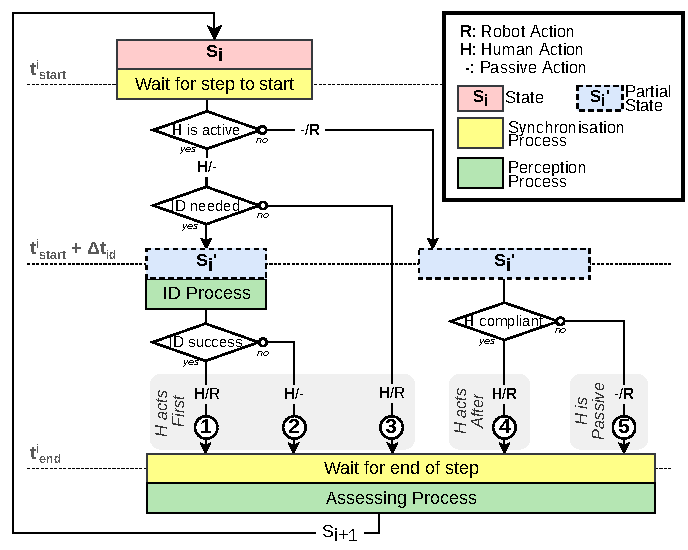
\includegraphics[width=\linewidth]{images/Chapter4/Execution_Automaton.drawio.pdf}
    \caption{
    The Model of Execution, in the form of an automaton and here simplified, captures the latitude of uncontrollable humans in their actions and guides our task planning approach.
    In this paradigm, the two agents can act concurrently but one is always compliant with the other's decision to act.
    Here, the human is always free to decide whether to start acting first, or after the robot, or not to act at all.
    To be compliant, the robot attempts to identify human decisions using perception and situation assessment as well as possible collaborative human signaling acts (e.g., gestures or speech).
    }
    \label{fig:model_of_execution}
\end{figure}

Our task planning approach uses a model of execution to improve the fluency and amenability of HRC. 
This model is in the form of an execution controller as shown in Figure~\ref{fig:model_of_execution}, and is based on several key notions and mechanisms borrowed from studies on joint actions~\cite{Sebanz-2016,kourtis2014attention}, and adapted to Human-Robot Joint Action~\cite{clodic-2017,curioni-2019}.
The key idea is that co-acting agents co-represent the shared task context and integrate task components of their co-actors into their own task representation~\cite{Schmitz-2017, Yamaguchi-19}. Also, coordination and role distribution rely strongly on reciprocal information flow, e.g., social signals~\cite{curioni-2019}, prediction of other's next action~\cite{luke-2018}.

Our proposed execution model is implemented on a robot that co-acts with a human, integrating explicit representation and exploration of the task representations for the robot and for the human. 
It also identifies precisely how reciprocal information flow is used in task execution (detecting and interpreting human actions, signals produced by the robot while acting, and also when the robot waits for human actions or their signals).

Another essential question is the criteria for choosing the next action, or more globally, how to share the load between the two co-actors. The choice depends on the context and actors' preferences~\cite{Gombolay-2015, Strachan-2020,Curioni-2022}. 
Concerning the case when one actor is a robot, we think it is important to provide a standard default behavior of the robot where the robot does its best to reduce human load but still leaves full latitude to act whenever humans want. 
Our scheme provides this ability and also allows humans to inform about their preferences at any moment.

Consider an example to clarify the execution automaton. 
Assume a human and a robot have to pick up two blocks, \textit{A} and \textit{B}, that both can reach. 
They can pick it up both at the same time unless they try to pick up the same block, which causes conflicts between their actions. 
As a result, despite being executable in parallel, the actions are interdependent, and in order to avoid conflicts, one agent must be compliant with the other. 
However, if we consider a third block \textit{C} that only the robot can reach, it can always pick up this block without any risk of conflicts with the human's choice. 

In a state, a human decision can result in one of three outcomes.
First, the human can choose to act first (\textit{left~subtree}).
If the robot's best action is not in conflict with the human action (e.g., \textit{pick~C}), the robot can safely perform this action concurrently with the human operator (\textit{branch~3}).
However, if the robot's best action is either \textit{pick~A} or \textit{pick~B}, the human action must be identified first with a subroutine in order to be compliant with it.
If this subroutine is successful the robot can perform any action which is congruent with the identified human action (\textit{branch~1}). 
This includes the robot's choice to be \textit{passive} and let the human act alone. 
However, if the robot is unable to identify the human action, it must remain passive in order to avoid potential conflicts (\textit{branch~2}). 
Then, the human can either decide to be \textit{passive} or to act after the robot (\textit{right~subtree}). 
In both cases, the human is \textit{passive} at the beginning, making the robot to start performing alone a feasible action. 
While the robot is acting, the human is free to remain \textit{passive} until the next step (\textit{branch~5}), or to choose a congruent action to act concurrently (\textit{branch~4}). 
As a result, the human can always choose to 1) act first, 2) act after the robot, or 3) not act at all. 
The robot will always be compliant with these online human decisions.

When both agents finish their actions, the step is considered as \textit{``over''}. 
Then, another subroutine assesses the new world state ($s_{i+1}$), which is the result of the concurrent actions being executed in the state $s_i$, before repeating the whole process until the task is solved.

Note that if both agents are passive (the human decides to be passive when the robot cannot act) then the step is repeated. 

\section{Exploration}

heavy, Offline

\subsection{compliant pairs}
\subsection{graph, merge state planning state}


\section{Policy generation}
Light, 

\subsection{Human preferences}
estimations, format, Discussion(often inaccurate, hence our Approach)

\subsection{process}
propagation + merge + policy format 

\section{Results}
simulation of execution, without durative action

\subsection{concept of aligned-adversarial pairs of prefs/estimations}

\subsection{results}

\section{Discussion and Limitations}
\section{Conclusion}





% \ifdefined\included
\else
\setcounter{chapter}{4} 
\dominitoc
\faketableofcontents
\fi

\chapter{Proactive Planning for unseen humans in the environment}
\chaptermark{Invisible Humans in HAN}
\label{chap:5}
\minitoc
\section{Introduction}
Most of the HAN frameworks~\cite{moller2021survey, kruse_ras_2013} address only the visible humans and do not take into account the possible emergence of humans that are not visible currently. We believe that such `\textit{invisible humans}' should be considered while developing a human-aware navigation framework to avoid any erratic behaviours of the robot planner when a human suddenly appears. Therefore in this chapter, we try to address these \textit{invisible humans} in HAN settings.

There is no work that addresses this problem in the field of HAN. However, there are some existing works in classical robot navigation that address similar issues. Particularly, this work is inspired by the pioneering work of M. Krishna~ \cite{madhavakrishna-ra-2006, alami-springer-2007, madhavakrishna-iros-2003} concerning the ability of a mobile robot, based on the model of its perception functions, to assess from where in the close environment of the robot a human can emerge and prepare to react to ensure no-collision by adapting its path and velocity. Some recent works like \cite{chung2009safe, Bouraine-2012} address the issues of robot navigation in occluded or unknown regions with a limited field of view. The work presented in \cite{miura2006adaptive} talks about the adaptive speed control of the robot in unknown environments and also talks about the occluded regions. The authors of \cite{lambert2008collision} propose a methodology to mitigate or avoid collisions while navigating. In our case, we are trying to mitigate possible future collisions with a human. 

As it is evident that the unknown or occluded region could cause issues with classical navigation, the same applies to HAN. Hence, we propose the concept of `\textit{invisible humans}' to HAN planning in this chapter. As per our knowledge, there is no other work that addresses this problem in a human-aware navigation context. Firstly, we formulate the problem of \textit{invisible humans} detection and propose an algorithm to determine the locations from which humans that are not currently visible can emerge suddenly. These \textit{invisible humans} are then integrated into our human-aware navigation framework, \acrshort{cohan} \cite{singamaneni2021human}, by introducing a new human-aware constraint into our optimization scheme. The constraint modifies the path and speed of the robot, taking into account the anticipation of potential human appearances to avoid collisions and surprises. This kind of preventive planning is also a part of the proactive planning approach as it mitigates the occurrence of potential problems. We further show how the detected \textit{invisible humans} can be exploited to identify some interesting places in a map, like doors or passages and address these by adding new modalities to \acrshort{cohan}. The implementation and code can be found at {\small {\url{https://github.com/sphanit/cohan_planner_multi/tree/model}}}. 

The organisation of this chapter is as follows. Section \ref{inv_human_detect} presents the formulation and an algorithm to detect \textit{invisible humans}. Section \ref{cohan_inv_human} shows how the \textit{invisible humans} are integrated into \acrshort{cohan} and talks about the issues that arise. It also presents a simple formulation to identify narrow passages. In section \ref{results_chap5}, various experiments to evaluate the proposed approach are presented, followed by the real-world experiments in section \ref{real_chap5}. A discussion on the limitations of this work is presented in section \ref{discussion_chap5}. Finally, section \ref{conclude_chap5} concludes this chapter.

% \section{The concept of `Invisible Humans’}
% \textcolor{red}{Explain about the idea and the concept in detail.}
\section{Invisible Humans Detection}\label{inv_human_detect}
The \textit{invisible humans} are detected using an emulated laser scan on a 2D map in ROS. A custom laser scan is attached to the robot's base, and it is continuously updated as the robot moves on a given map. The entire system is implemented in ROS \cite{quigley2009ros} and requires the map that is published by the ROS Navigation Stack. In order to avoid too many detections, we limit the \textit{invisible humans} detection to a radius of \SI{5}{\meter} in front of the robot. The detection of \textit{invisible humans} is a two-step process involving corner detection and locating invisible humans. Each step is explained in detail below.

\subsection{Corner Detection using Laser Contour}
A custom laser scan sensor attached to the robot's base scans the given 2D map to get the visible contour of the map. The laser data consists of a list of values showing the scan ranges in the field of vision of the sensor. The custom sensor data is used in place of the real laser scan data to ensure uniformity across different robots and sensors. An example laser contour built using this is shown in Fig. \ref{fig:detection}. Different parts of these contour lines are shown in different colours for ease of explanation. The red and the blue lines together constitute the regions on the real map where the laser has hit a wall or an obstacle. The black lines represent the laser data that did not hit anything and reached the end of their range (in our case, the range of the laser is \SI{7}{\meter}). Lastly, the yellow lines are interpolated rays joining large separations between consecutive laser values and play a major role in our algorithm. The red circle and the arrow represent the robot's position and direction, while the green circles represent the estimated \textit{invisible humans}. Corner detection is relatively easy once the laser contour is available. Firstly, all the pairs of consecutive laser range values separated by more than \SI{0.5}{\meter} are determined and stored in a set \{$V$\}. The threshold of \SI{0.5}{\meter} is chosen to filter out small gaps from where a human will not emerge. After this, the values closest to the robot's position in each of the above pairs are identified to be corners of interest and stored in a set \{$c$\}. These are shown as yellow circles in Fig. \ref{fig:detection}.
\begin{figure}[h!]
    \centering
    \begin{subfigure}[t]{0.45\columnwidth}
    \centering
  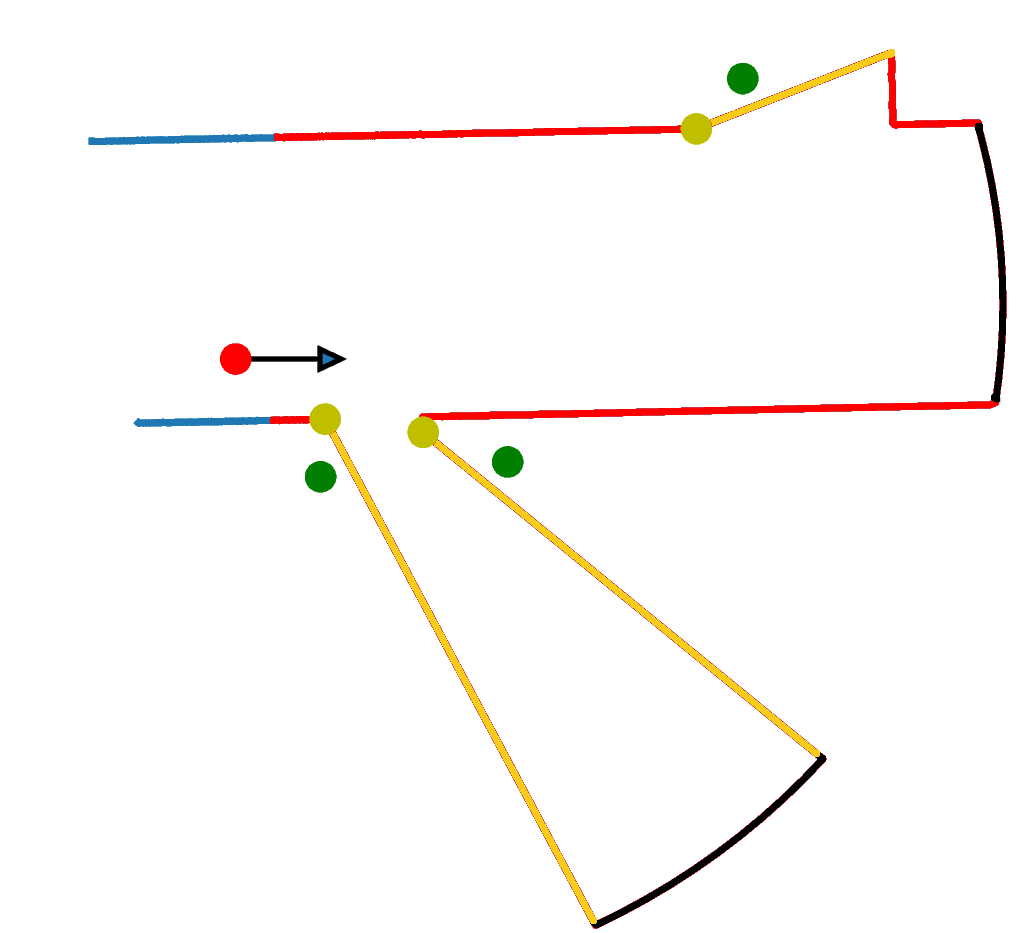
\includegraphics[width=\columnwidth]{images/chapter5/detection.png}
  \caption{Laser Contour}
\end{subfigure}
\begin{subfigure}[t]{0.45\columnwidth}
\centering
  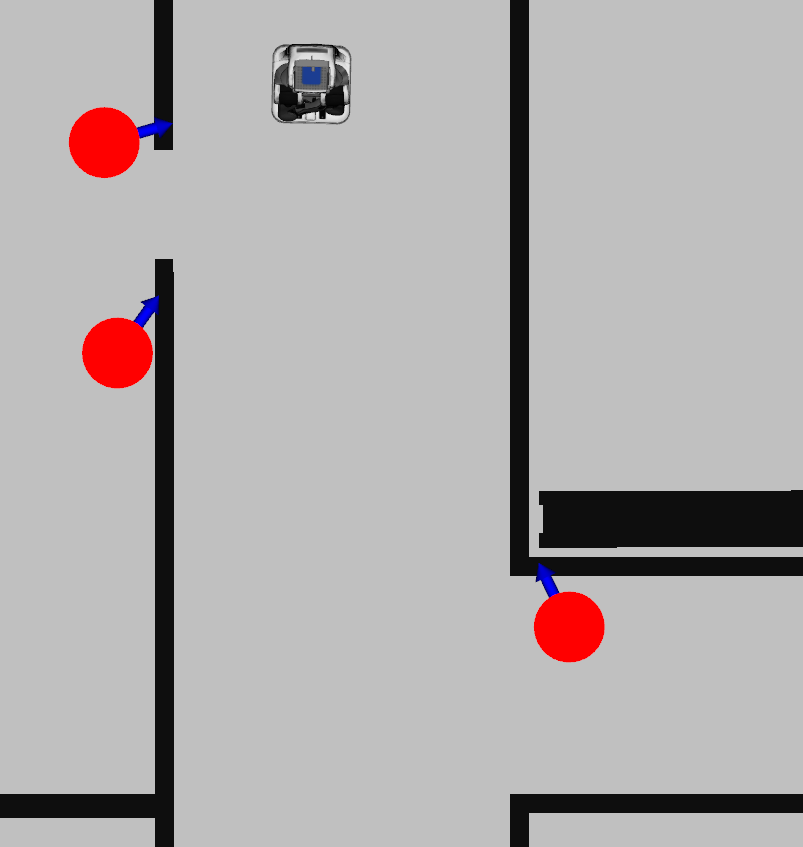
\includegraphics[width=0.8\textwidth]{images/chapter5/detection_rviz.png} 
  \caption{Detected \textit{invisible humans}}
\end{subfigure}
    \caption{(a) Laser contour built by the custom laser sensor. The red and blue lines are the actual walls or obstacles in the front and back of the robot respectively. The black lines are the laser range boundaries and the yellow lines are interpolated lines between two gaps of laser data. The robot is shown as a red dot with an arrow. The detected corners are shown in yellow, while the detected \textit{invisible humans} are shown in green. (b) The detected \textit{invisible humans} on the map for the contour shown. The red circles shows the location and the blue arrow shows the assumed direction, which is always oriented towards the robot.}
    \label{fig:detection}
\end{figure}

\subsection{Estimation of Invisible Humans’ Locations}
The estimation of possible locations for the \textit{invisible humans} is not very straightforward. The laser contour forms a complex non-convex polygon, and we are searching for circles whose centres are outside this polygon and do not intersect the contour. We solve this problem using a combination of ray tracing and vector algebra. Consider a non-convex polygon as shown in Fig. \ref{fig:polyg}. The vertices are numbered in the anti-clockwise direction. Consider a point $P_1$ that lies between the vertices $V_1$ and $V_2$. If $P_1$ is outside the polygon, it should lie to the right of the vector $\overrightarrow{V_1V_2}$. Similarly, a point $P_2$ lying outside the polygon between $V_2$ and $V_3$ lies to the right of $\overrightarrow{V_2V_3}$ and so on. It holds true irrespective of the number of sides of the polygon. We exploit this property to determine the positions of the \textit{invisible humans}. Note that a point lying outside the polygon will always be on the right side of the vectors, but not every point on the right of the vectors lies outside the polygon. This is because the methodology uses only a single side and does not consider the other sides. To handle this, we use the fact that the polygon, in our case, is determined by the laser contour, and any point outside this polygon is not visible to the laser.

\begin{figure}[h!]
\centering
\begin{subfigure}{.55\columnwidth}
  % include first image
  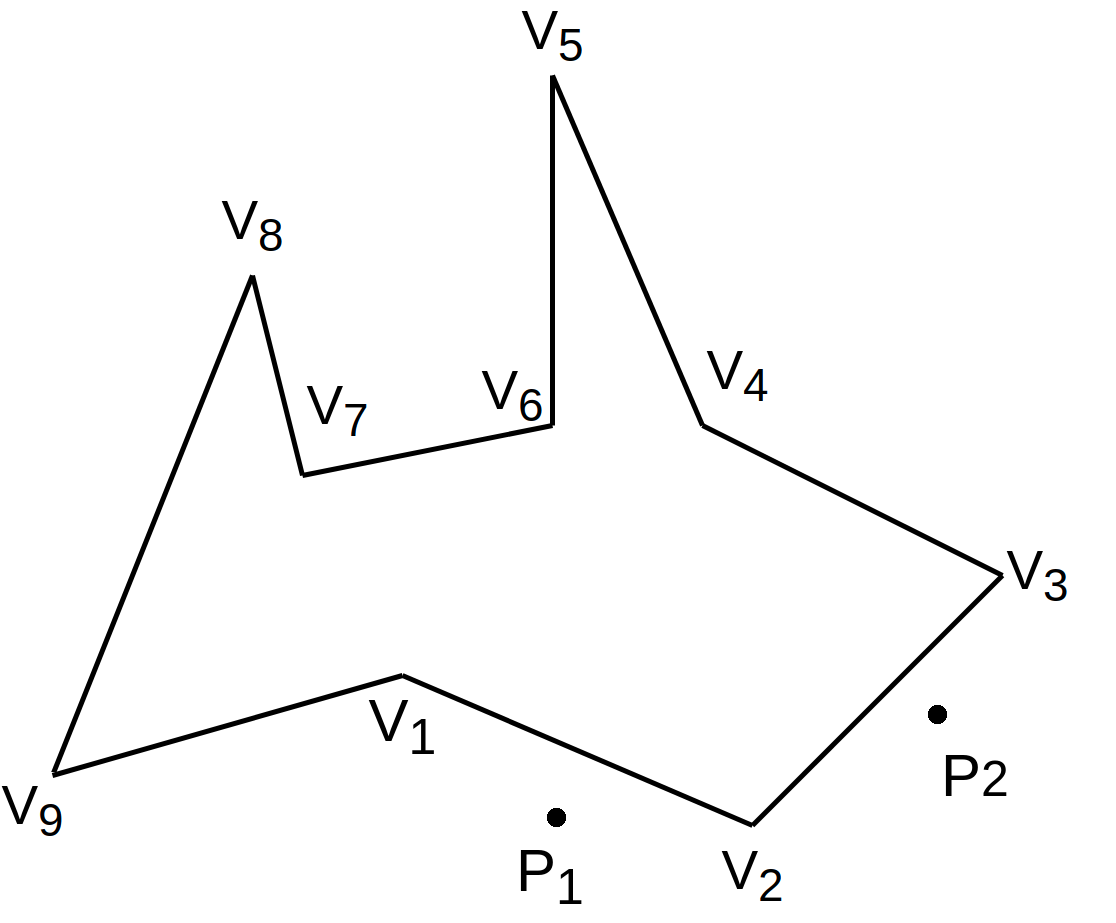
\includegraphics[width=0.8\textwidth]{images/chapter5/polygon.png}
\end{subfigure}
\hspace{-0.5cm}
\begin{subfigure}{.35\columnwidth}
%   \centering
  % include second image
  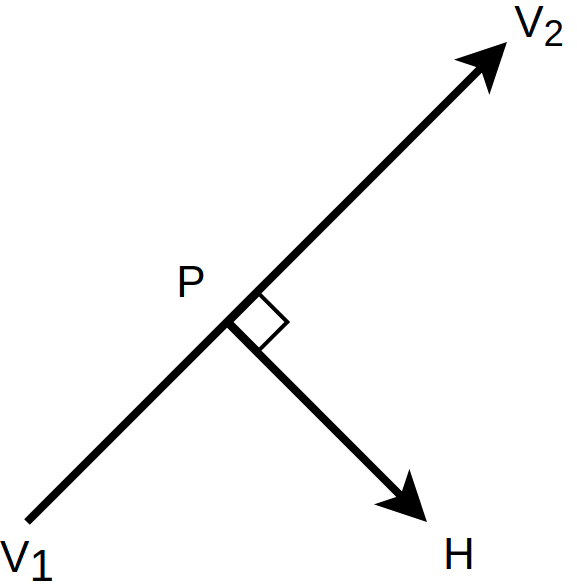
\includegraphics[width=0.8\textwidth]{images/chapter5/vectors.png} 
\end{subfigure}
\caption{Non-convex polygon and vector formulation to determine \textit{invisible humans}. We try to find a point {$H$} that lies between two vertices {$V_1$} and {$V_2$} and lies to the right of $\overrightarrow{V_1V_2}$. Note that the perpendicular distance of this point should be greater than the assumed human radius.}
\label{fig:polyg}
\end{figure} 

In Fig. \ref{fig:detection}, the yellow lines correspond to the edges of interest in the polygon. The numbering of the vertices is determined based on the indices of the laser scan data, which (the rays) move from right to left in the anti-clockwise direction. In order to determine a possible invisible human, we need to determine a point $H$ that is to the right of $\overrightarrow{V_1V_2}$ and whose perpendicular distance is greater than an average human radius, $h_{rad}$ as shown in Fig. \ref{fig:polyg}. Consider a point $P$ that lies on line segment $\overline{V_1V_2}$ such that $\overrightarrow{PH}$ is perpendicular to $\overrightarrow{V_1V_2}$. If we know the point $P$, then $H$ can be determined using the following equations:

\begin{equation}\label{chap5_eq1}
       sign(\overrightarrow{V_1V_2}\times\overrightarrow{PH}) = -1
\end{equation}
\begin{equation}\label{chap5_eq2}
    \overrightarrow{V_1V_2}\cdot\overrightarrow{PH} = 0
\end{equation}
\begin{equation}\label{chap5_eq3}
           \lVert\overrightarrow{PH}\rVert = h_{rad}+\epsilon
\end{equation}
where ($\times$) is the cross product, ($\cdot$) is the dot product and ($\lVert \rVert$) is the euclidean norm, respectively. $\epsilon$ is the offset on the human radius to avoid unrealistic detections. In this work, we chose $\epsilon$ to be $\frac{h_{rad}}{2}$. Let $V_1$ = $(x_1, y_1)$, $V_2$ = $(x_2, y_2)$ and $P$ = $(x_p, y_p)$, then by solving the above equations, $H$ = $(x_{h}, y_{h})$ is given by:
\begin{equation}\label{chap5_eq4}
  \begin{aligned}
        x_{h} = x_p + \frac{d(y_2-y_1)}{\sqrt{(x_2-x1)^2+(y_2-y1)^2}} \\
        y_{h} = y_p - \frac{d(x_2-x_1)}{\sqrt{(x_2-x1)^2+(y_2-y1)^2}}  
  \end{aligned}
\end{equation}
where $d = (h_{rad}+\epsilon)$. Similarly, the point on the left can be obtained by reversing the sign in Eq.~\eqref{chap5_eq1}, which yields: 
\begin{equation}\label{chap5_eq5}
  \begin{aligned}
        x_{h} = x_p - \frac{d(y_2-y_1)}{\sqrt{(x_2-x1)^2+(y_2-y1)^2}} \\
        y_{h} = y_p + \frac{d(x_2-x_1)}{\sqrt{(x_2-x1)^2+(y_2-y1)^2}}  
  \end{aligned}
\end{equation}

From the Eq.~\eqref{chap5_eq4}, we can see that $(x_p,y_p)$ is required to determine $(x_h,y_h)$ and it is still unknown as we cannot solve for four variables using only two equations (Eq.~\eqref{chap5_eq1}-\eqref{chap5_eq2}). As it is already known that $P$ lies on the line segment joining $\overline{V_1V_2}$, it can be determined by performing a search on this line segment, starting at one end and moving towards the other in small increments. The set of detected corners, \{$c$\}, are taken as the starting points of this search. In each iteration, a possible invisible human position is estimated using Eq.~\eqref{chap5_eq4} and then projected onto the map to see if there is any overlap with an obstacle or wall. As mentioned before, we need another check to ensure that the point is outside the laser contour. Suppose the vector joining the robot and the point $H$ is $\overrightarrow{r}$, and it subtends an angle $\beta$ with the positive $x-axis$ of the base frame of the robot. As the custom laser is also attached to the base frame of the robot, there should be laser scan data corresponding to this angle $\beta$. Hence, when the $H$ is outside, the following condition is satisfied:
\begin{equation}
    \lVert\overrightarrow{r}\rVert > \rho(\beta)
\end{equation}
where $\beta = atan2(x_h - x_{rb},\ y_h-y_{rb})$, $(x_{rb}, y_{rb})$ is the robot base frame's position and $\rho(\beta)$ is the laser scan reading at angle $\beta$. To refine this search further, two points, one on the left, $P_l$, and the other on the right, $P_r$, of the $H$ are considered with incremental distances until $h_{rad}+\epsilon$ and checked for overlap using the map. 

The entire procedure is shown in Algorithm \ref{algo} where $u_x$ and $u_y$ (line 6) are the unit vectors along the direction of $\overrightarrow{V_1V_2}$ and $\alpha$ is a scalar determining (lines 32, 33) the step size or increment.
\begin{algorithm}
\caption{Locate Invisible Humans}\label{algo}
\begin{algorithmic}[1]
% \Function{FindMeshIndex}{$\vars{position}, \vars{nGrid}$}
\State Determine the vertex pairs set \{$V$\} using laser contour
\State Determine the corners set \{$c$\} from \{$V$\}
\For {each $c$} 
\State $V_1$ = $c$ = $(x_1,y_1)$
\State $V_2$ = $(x_2, y_2)$ \Comment{Corresponding pair from \{$V$\}}
\State $u_x = \frac{(x_2-x_1)}{\lVert\overrightarrow{V_1V_2}\rVert}$, $u_y = \frac{(y_2-y_1)}{\lVert\overrightarrow{V_1V_2}\rVert}$ 
\State Set $P$ = $(x_p,y_p)$ = $(x_1,y_1)$
\While{True}
\State Calculate $H_{inv}$ using Eq.~\eqref{chap5_eq4}
\State Calculate $\overrightarrow{r}$ and $\beta$
\If{$\lVert\overrightarrow{r}\rVert < LaserData(\beta)$}
\State $x_p = x_p + \alpha u_x$
\State $y_p = y_p + \alpha u_y$
\State continue
\EndIf
\State Check for overlap on the Map
\If{no overlap}
\State $advance = False$
\For{$i = 1$ to $k$}
\State $d = \frac{i}{k}* (h_{rad}+\epsilon)$
\State Calculate $P_r$ and $P_l$ using Eqs.~\eqref{chap5_eq4}, \eqref{chap5_eq5}
\State Check $P_r$, $P_l$ for the overlap on Map 
\If{no overlap}
\State continue
\ElsIf{overlap}
\State $advance = True$
\State break
\EndIf
\EndFor
\EndIf
\If{$advance == True$}
\State $x_p = x_p + \alpha u_x$
\State $y_p = y_p + \alpha u_y$
\ElsIf{$advance == False$}
\State break
\EndIf
\EndWhile
\State Add $H_{inv}$ to the set of \textit{invisible humans}, \{$H_{inv}$\}
\EndFor
\State \textbf{return} \{$H_{inv}$\}
\end{algorithmic}
\end{algorithm}
The \textit{invisible humans} detected using the above-mentioned algorithm are shown in Fig. \ref{fig:detection} (b). The red circles are the detected location, while the blue arrows show the direction. We assume that the humans are always coming towards the robot, and hence, the direction is always oriented towards the robot. In the next section, we explain how this is integrated into the human-aware planning framework for social robot navigation.  


\section{Introducing Invisible Humans into CoHAN}\label{cohan_inv_human}
In the previous version of \acrshort{cohan}, we address different types of visible humans by introducing new modalities and human-aware constraints~\cite{singamaneni2021human}. In this chapter, we extend it further to address the~\textit{invisible humans}. The \textit{invisible humans} are detected as explained above, and then they are published on a ROS topic. \acrshort{cohan} subscribes to this topic and adds a new constraint to its optimization that is specifically designed for \textit{invisible humans}. Note that we do not add any elastic band and only add an `invisible human-aware' constraint to make the robot proactively plan its trajectory. Further, using these invisible human detections, we propose a methodology to identify doors and narrow passages.

\subsection{The `Invisible Humans Constraint’}
The \textit{invisible humans} constraint takes into account the human reaction time, walking speed, and deceleration. It aims to make the robot cautious about sudden human emergence. The cost added by this constraint for the n\textsuperscript{th} pose of the robot's trajectory is given as:
\begin{equation}
\begin{split}
cost_{inv\_human} &= max\left(\frac{V-a\Delta t_n}{d}, 0\right)\quad \text{if}\quad \Delta t_n> 0.5s\\
                &= \frac{V}{d}\quad otherwise
\end{split}
\label{cost_}
\end{equation}

where $d$ is the distance between the invisible human and the robot, $V$ is the average human walking speed, \SI[per-mode=symbol]{1.3}{\meter\per\second} \cite{phdthesis}, $a$ is the deceleration of the human, and $\Delta t_n$ is the time difference between the n\textsuperscript{th} pose and the starting pose of the planned trajectory of the robot. The value of the deceleration, $a$, can vary and can be up to a maximum of \SI{2.94}{\meter\per\second^2} (\SI{0.3}{\g}) \cite{lakoba2005modifications}. In this work we take a reaction time of \SI{0.5}{\second} as discussed in \cite{lakoba2005modifications, helbing2000simulating}. Hence the constraint adds the maximum possible cost until \SI{0.5}{\second}. Then we assume that the human will continuously decelerate to avoid collision with the robot over time and eventually stops, which is reflected in the upper part of Eq. \eqref{cost_}. The time ($\Delta t$) and human detections are reset after every control cycle. The above cost makes the optimization to produce a trajectory that makes the robot take larger turns around the corners and other openings from where a human might emerge (if detected by the presented algorithm). Hence, our HAN system proactively mitigates potential collisions with unseen humans, and we believe that it is a more acceptable way than reacting after seeing a human.  

\subsubsection{Issue with the Constraint}
The main objective of the constraint is to push the robot away from the opening, anticipating the emergence of \textit{invisible humans}. However, when the robot needs to pass through this opening and if the passage is narrow (door or narrow corridor), the constraint pushes the robot away and makes it impossible to enter the passage. To mitigate this, we devise a simple formulation that detects such scenarios. Once a narrow passage is detected, the \textit{invisible humans} constraint is switched off, and the maximum robot's velocity is reduced until it passes through. The passage detection process is explained in detail in section~\ref{psg_detect}.

\subsection{Passage Detection and a New CoHAN Planning Mode}\label{psg_detect}
The detection of narrow passages or doorways not only allows us to overcome the issue of the \textit{invisible humans} constraint but also to define a new modality of planning that needs to be handled separately. In this work, we try to address three different scenarios, as shown in Fig. \ref{fig:passages}.  
\begin{figure}[h]
    \centering
    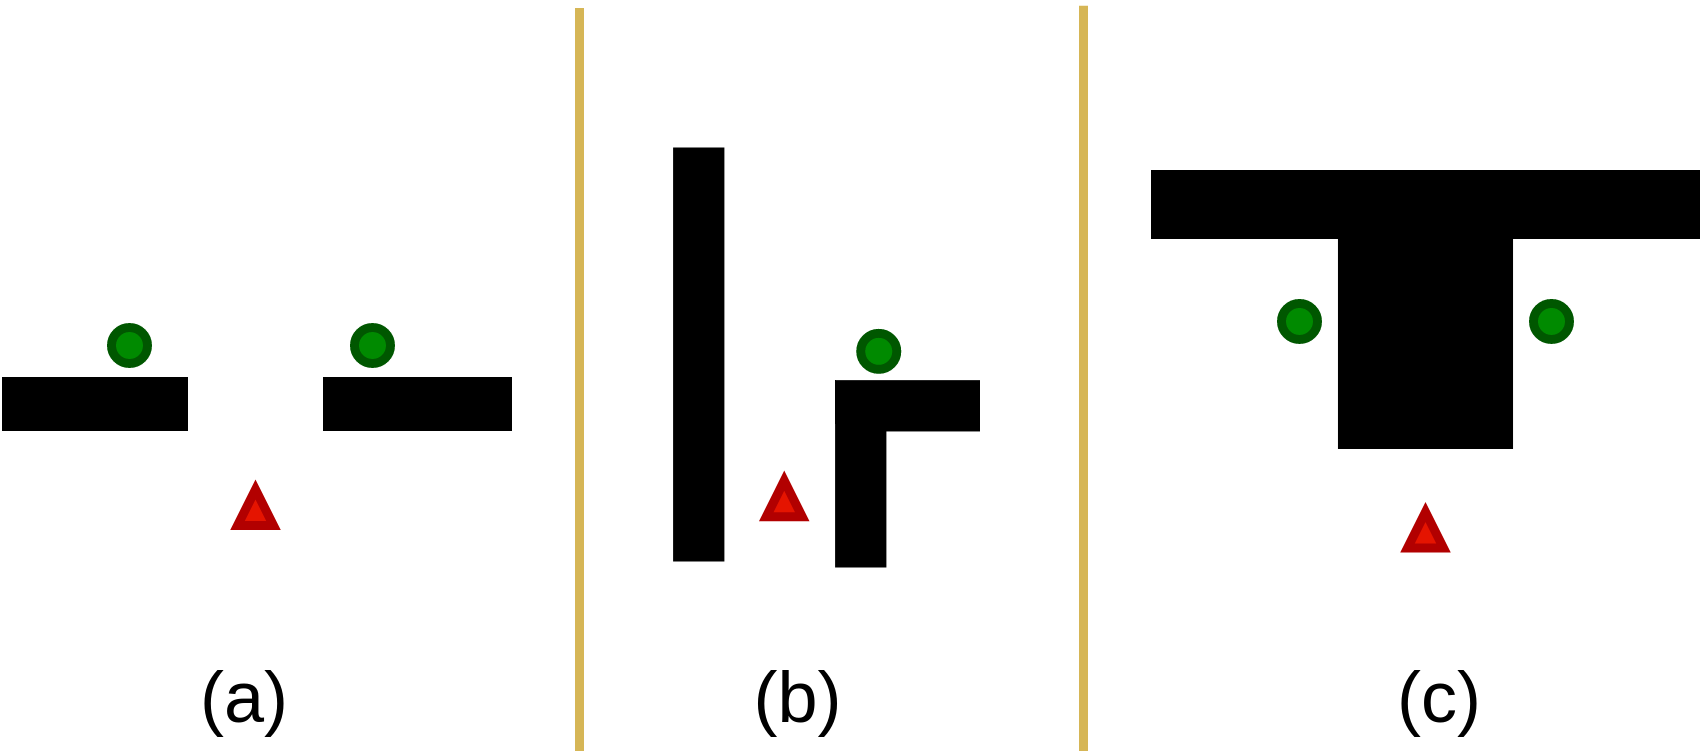
\includegraphics[width=0.8\columnwidth]{images/chapter5/passages.png}
    \caption{Different types of passages that are detected using \textit{invisible humans}. (a) Doorways or openings and endings of the corridors (b) a narrow passage with opening on one side and a wall on the other side (c) a large pillar or obstacle where robot cannot see on either side. The green circles are the possible locations of the \textit{invisible humans} and the red triangle shows the robot pointed towards the direction of its motion.}
    \label{fig:passages}
\end{figure}
The first scenario, Fig. \ref{fig:passages} (a), occurs in the case of a doorway or the openings and closings of a narrow passage. In such scenarios, the \textit{invisible humans} exert equal forces from two different directions, which align the robot at the centre of the passage. If the opening is narrow, the resultant force is strong and does not let the robot pass through until the invisible constraint turns off. However, the threat of \textit{invisible humans} still exists, so the robot should act cautiously. Therefore, we make the robot move slowly with a lower velocity ($\leq$ \SI{0.3}{\meter\per\second}) until it passes through the passage. To detect this scenario, we use the positions of the \textit{invisible humans} and the robot to check whether an \textit{isosceles triangle} is formed with the three vertices. The robot lies on the vertex, which connects the approximately equal sides, and humans at the base vertices. In order to limit false detections, we set some numerical limits on the lengths of the equal sides and the base. Assuming that a human has \SI{0.3}{\meter} radius and the robot has \SI{0.5}{\meter}, the length of the base should be $\geq$ \SI{1.6}{\meter}. When the clearance from obstacles or walls is taken into account, it increases further. In this work, we set the limit on base length as \SI{3}{\meter}. Similarly, for the equal sides, there should be a minimum length of \SI{0.8}{\meter}, and we chose the limit to be \SI{2}{\meter}. These values are chosen empirically based on the tests in several situations. If the above conditions are satisfied, a passage is detected, and \acrshort{cohan} switches to a new modality called \textbf{Pass Through}, which sets the conditions mentioned above. This mode can be activated at any time and in any of the planning modes of \acrshort{cohan}. Therefore, it can be seen as an asynchronous planning mode that can be triggered at any time, unlike the previous planning modes, and hence, it is independent of the situation assessment loop in \acrshort{cohan}. The situation shown in Fig. \ref{fig:passages} (c) is almost the same as the doorway. It is differentiated from the doorway case by reading the centre value of the laser scan data. If the value in the data is less than the length of the perpendicular bisector of the triangle's base, it is identified as a pillar or a large obstacle. \acrshort{cohan} identifies this as a new case, but for now, we handle it the same we handle the doorway.

The situation shown in Fig. \ref{fig:passages} (b) is different from the other two as the robot's passage is blocked on one side by an invisible human and an obstacle on the other. As the robot may or may not align in this case, it must be handled differently. We check the angle of the laser scan corresponding to the detected corner and read the value of the data that is symmetrical to this angle along the direction of the robot. If the difference between the distance of this laser scan data and the invisible human from the robot's position is $\geq$ \SI{1}{\meter}, we identify it as a wall passage and set \acrshort{cohan} to \textbf{Pass Through} mode once again. The threshold of \SI{1}{\meter} is chosen empirically here.

\section{Results} \label{results_chap5}
The proposed approach is tested in several settings after being completely integrated with \acrshort{cohan}. In this section, we show four interesting scenarios and present a detailed analysis. In all these experiments, we assume $h_{rad}= $\SI{0.3}{\meter} and set $k=10$ and $\alpha=0.2$. We use ROS-melodic with Ubuntu 18.04, and all the scenarios are simulated using MORSE~\cite{echeverria2011modular} simulator. The simulated human agents used in the experiments are controlled using InHuS~\cite{favier2021intelligent}, a human simulator developed in our lab.

\subsection{The Effect of the Invisible Humans Constraint}
We demonstrate the advantage of introducing proactive planning around the \textit{invisible humans} with two different scenarios. A detailed analysis of these scenarios with and without the proposed constraint is presented. Subsequently, a comparison with some of the planners in \textbf{\textit{move\_base}} shows how the proposed approach can improve human comfort.

\subsubsection{Door Crossing Scenario}
\begin{figure}[!h]
    \centering
    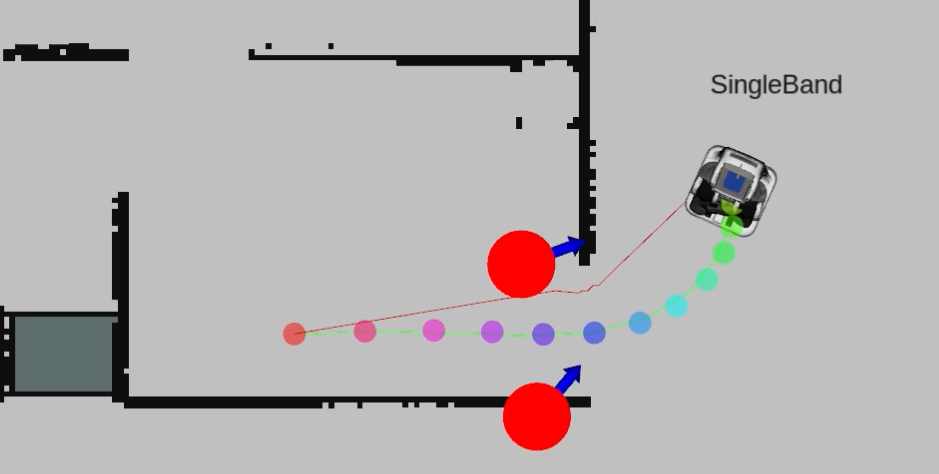
\includegraphics[width=0.8\columnwidth]{images/chapter5/door_secne.png}
    \caption{The robot passing through the door under the presence of \textit{invisible humans}. The colored circles represent the poses of the robot and different color corresponds to different time instance.}
    \label{fig:door_scene}
\end{figure}
\begin{figure}[!h]
\centering
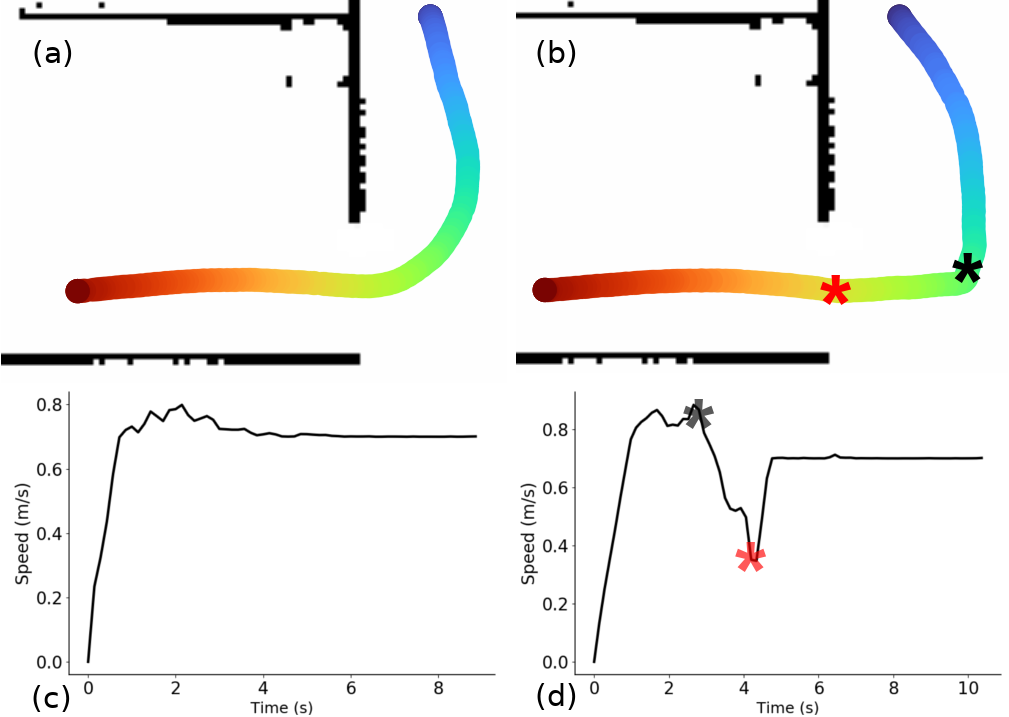
\includegraphics[width=0.85\columnwidth]{images/chapter5/door_new.png}
\caption{Paths and speed profiles of the robot passing the door without (a, c) and with (b, d) the \textit{invisible humans} constraint. The color of the paths indicates the time and progress of the robot, from blue to red (start to goal). In (a) the robot crosses the door “full speed”. In (b) it decelerates before entering the door (black star) and has the lowest speed at the entrance to the door (red star) around $4.2s$ corresponding to the shortest distance to \textit{invisible humans}.}
\label{fig:door_constraint}
\end{figure}
To show the effect of introducing the \textit{invisible humans} constraint into \acrshort{cohan}, we present the robot with a door crossing scenario as shown in Fig. \ref{fig:door_scene}. We test the scenario without and with the \textit{invisible humans} constraint and the corresponding paths of the robot are presented in Fig. \ref{fig:door_constraint} (a)  and Fig. \ref{fig:door_constraint} (b) respectively. The paths are coloured, and the colour moves from blue to red as the robot moves from start to goal. It can be seen from these paths that the inclusion of the constraint made the robot more cautious as it takes a larger turn and aligns its path before passing through the doorway. 

The corresponding speed plots are shown in Fig. \ref{fig:door_constraint} (c) and (d). Comparing the plot in Fig. \ref{fig:door_constraint} (d) with the speed profile in Fig. \ref{fig:door_constraint} (c), it can be seen that the robot, after aligning itself with the entrance, starts decelerating slowly (black star) as it moves towards the door. At the door, there is a sharp deceleration again, and the robot passes this place (red star) at the lowest speed. This clearly reflects the cautious behaviour of the robot.


\subsubsection{Sudden Emergence of a Human}
 \begin{figure}[!h]
    \centering
    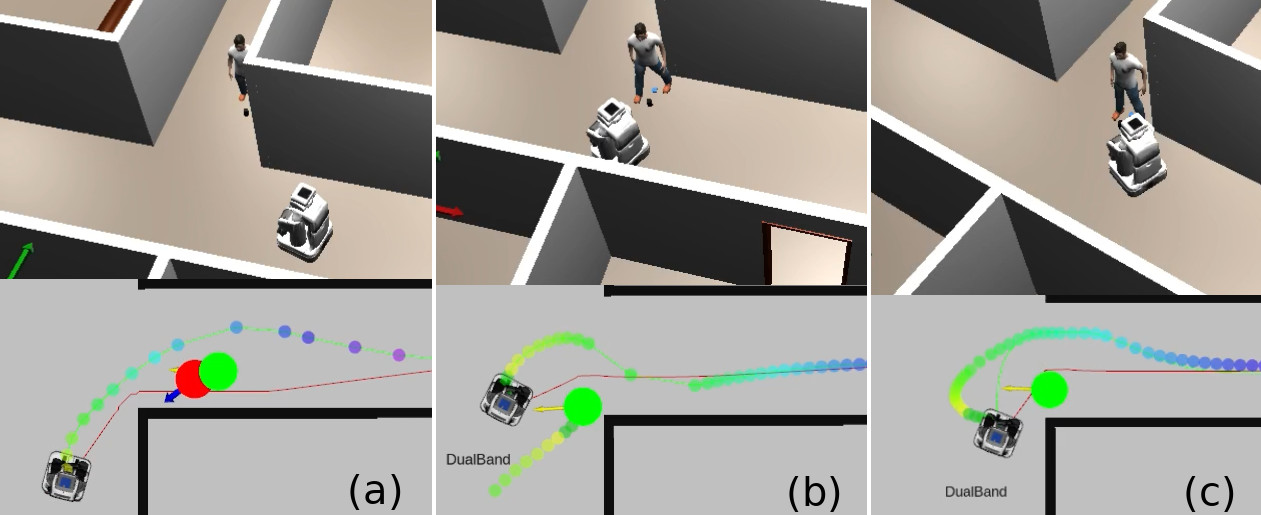
\includegraphics[width=0.9 \columnwidth]{images/chapter5/appear_scene_final_new}
    \caption{Sudden emergence scenario.  The colored paths with circles is the planned trajectory of the robot. (a) Shows the anticipated invisible human in red and the real human in green. The robot starts moving away from the corner. (b) The robot has seen the human and adjusted its trajectory to provide more space to the human. (c) The scenario without the \textit{invisible humans} constraint. The robot moves very near to the wall blocks the human momentarily before adapting its path.}
    \label{fig:emergence}
\end{figure}

\noindent The next scenario we discuss in this section shows a situation where a human emerges suddenly from an occluded region. The snapshots of this scenario before and after the emergence are shown in Fig. \ref{fig:emergence}. The added \textit{invisible humans} detection predicts a possible position of the human as shown in Fig. \ref{fig:emergence} (a), which approximately overlaps with the real human. The robot starts moving away from the wall slowly because of this anticipation, and suddenly a real human appears in front of it (Fig. \ref{fig:emergence} (b)). The robot quickly adapts its trajectory and moves away from the human, slowing down a little before continuing to its goal. However, without this detection, as shown in Fig. \ref{fig:emergence} (c), the robot moves close to the wall and blocks the human's way for a moment before changing its path. The paths taken by the robot without and with the addition of \textit{invisible humans} constraint to \acrshort{cohan} are shown in Fig. \ref{fig:appear_plots} (a) and Fig. \ref{fig:appear_plots} (c) respectively. It is clear from these plots that the proposed constraint makes the robot move cautiously and lessens the surprise to humans. Further, the path of the robot is smoother in Fig. \ref{fig:appear_plots} (c) when compared to the path in Fig. \ref{fig:appear_plots} (a) as there are no sudden path changes. 

\begin{figure}[ht!]
\centering
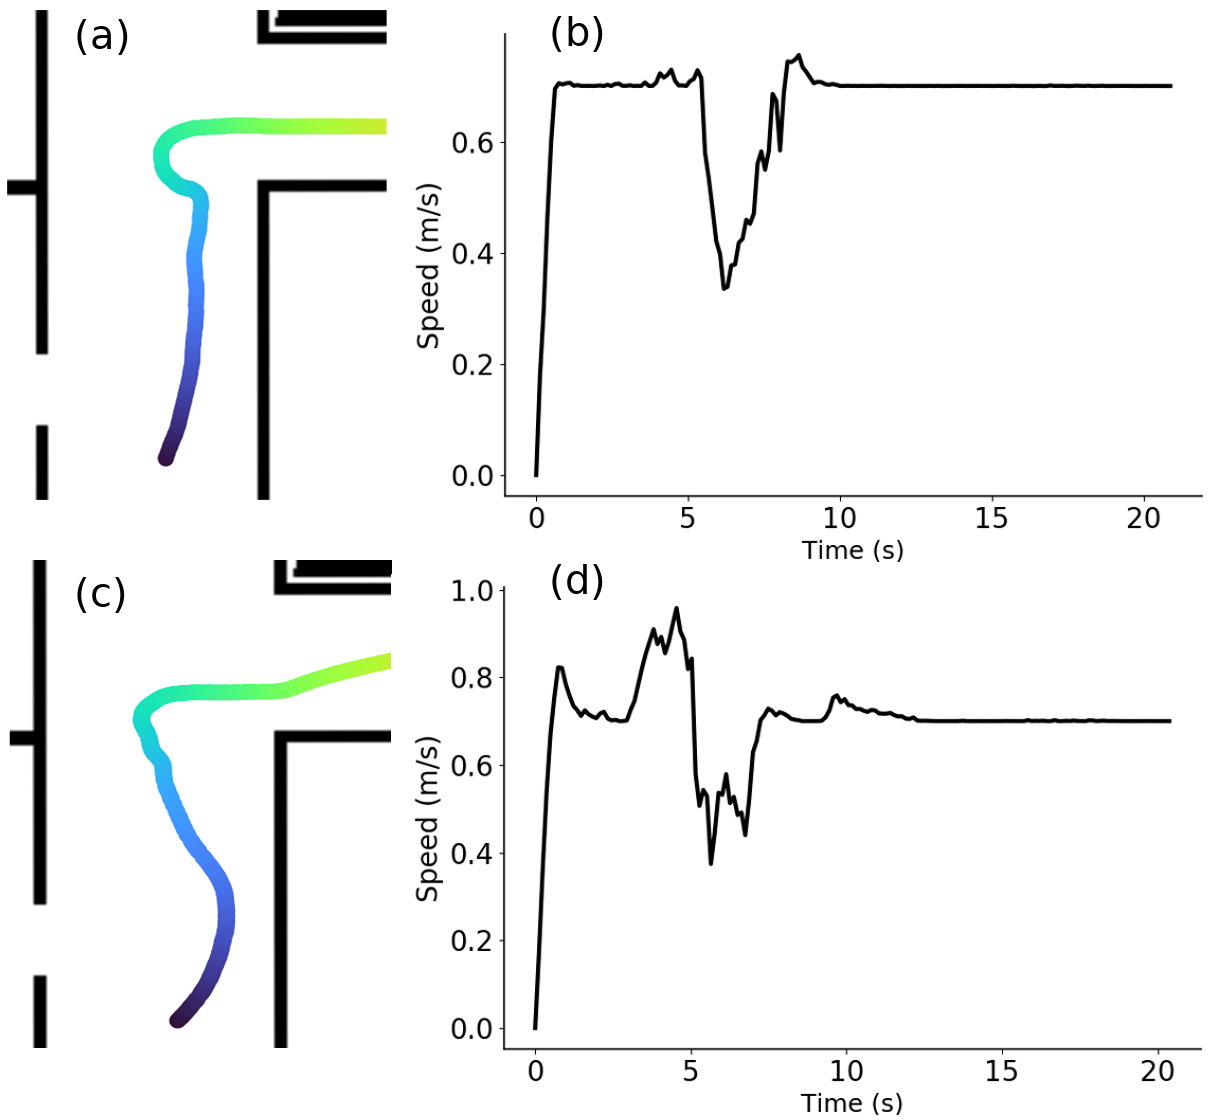
\includegraphics[width=0.8\columnwidth]{images/chapter5/appear_new.png}
\caption{Path and speed profiles of the sudden emergence scenario without (a, b) and with (c, d) the \textit{invisible humans} constraint. The color of the path indicates the time and progress of the robot, from blue to green (start to goal).}
\label{fig:appear_plots}
\end{figure}

The speed profile in Fig. \ref{fig:appear_plots} (b) shows a sudden drop in the velocity of the robot. This occurs because \acrshort{cohan} adapts its speed to prevent a possible collision and shock to the human. Then, the robot slowly moves away and plans a new path to the goal. The speed profile in Fig. \ref{fig:appear_plots} (d) is completely different compared to the last one. The robot starts drifting away from the wall (both x and y velocities) before seeing the human, and this shows the increase in the velocity. When the human appears, it slows down and then changes its direction before continuing to the goal with almost a constant speed. This is the sharp change (slowdown) we see in Fig. \ref{fig:appear_plots} (d) between $5$ and $10$ seconds.


\subsubsection{Comparison with Other Planners}
To test the effectiveness of the proposed approach, we compare the sudden emergence scenario using three different planners. The first one is Simple Move Base (SMB), where humans are added using the laser scan. Then we use \acrshort{cohan} with and without the proposed constraint as the other two planners. As the proposed work makes the robot cautious and tries to reduce the surprise to humans, we check the minimum human-robot distance while navigating using these planners. We have performed 5 runs of the same scenario with each planner, and the results are presented in Table \ref{compare_table}. From Table \ref{compare_table}, we can see that adding the \textit{invisible humans} constraint to \acrshort{cohan} makes the robot maintain a larger distance from the human around a corner. Keeping distance from humans avoids surprise to humans and provides time for the robot planner to adapt slowly.
\begin{table}[h!]
    \centering
    \begin{tabular}{|l|c|}
    \hline
    \textbf{Planners} & \textbf{Min. Human-Robot Distance ($m$)}\\
    \hline
      \textit{SMB} & 0.58\\
    \hline
     \textit{CoHAN} & 0.92\\
    \hline
     \textit{CoHAN with constraint} & 1.25\\
    \hline
    \end{tabular}
    \caption{Results of sudden emergence scenario using 3 different planners.}
    \label{compare_table}
\end{table}

\subsection{Navigating in the Presence of Visible and Invisible Humans}
\begin{figure}[h!]
    \centering
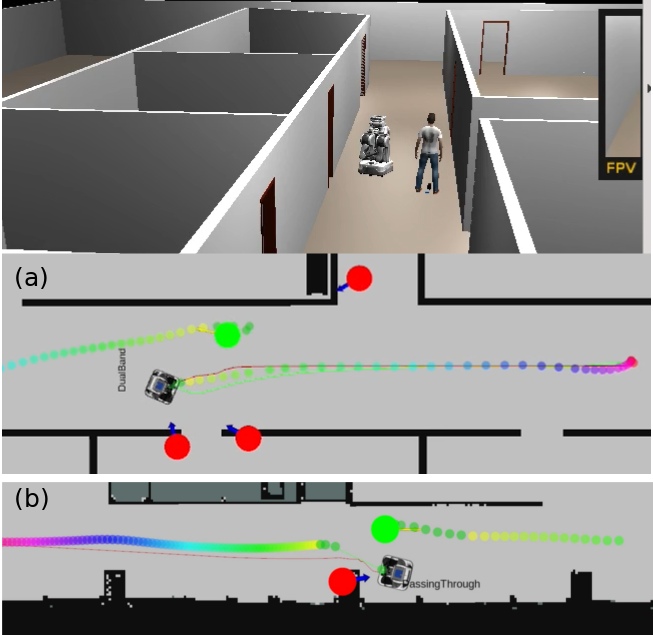
\includegraphics[width=0.8\columnwidth]{images/chapter5/corridors_new}
    \caption{Corridor scenarios used for testing CoHAN. (a) Corridor with many openings where the robot continuously anticipates the emergence of humans. (b) Corridor with pillars between passage that creates complex navigation scenarios. In both these settings, the robot tries to find a balance between visible and \textit{invisible humans}. The green circle is the visible human interacting with the robot, while the red circles are estimated \textit{invisible humans}. The coloured path with circles is the planned trajectory of the robot.}
        \label{fig:corridor_scene}
\end{figure}
\noindent The inclusion of the \textit{invisible humans} into human-aware navigation planning should not cause discomfort to the visible humans that are moving around the robot. To show that \acrshort{cohan} finds a balance between the invisible and visible humans, we present two corridor scenarios, one with many doors (or openings) as shown in Fig. \ref{fig:corridor_scene} (a) and the other with pillars as shown in Fig. \ref{fig:corridor_scene} (b). In both of these scenarios, the robot faces complex situations where it has to find a balance between the visible and the \textit{invisible humans}.

% Useful for Subfigures
\begin{figure}[b!]
\begin{subfigure}{\columnwidth}
  \centering
  % include first image
  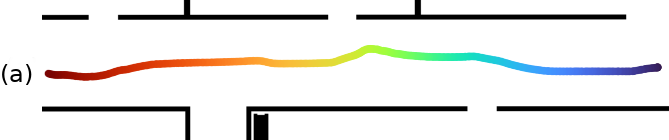
\includegraphics[width=0.8\textwidth]{images/chapter5/corridor_path_new.png}
%   \caption{Path: Many openings corridor}
\end{subfigure}
\hspace{-0.17cm}
\begin{subfigure}{\columnwidth}
  \centering
  % include second image
  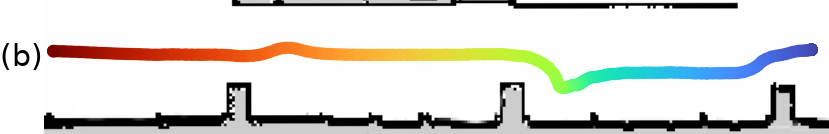
\includegraphics[width=0.8\textwidth]{images/chapter5/pillar_new.png} 
%   \caption{Path: Pillar Corridor}
\end{subfigure}
\begin{subfigure}{0.45\columnwidth}
  \centering
  % include first image
  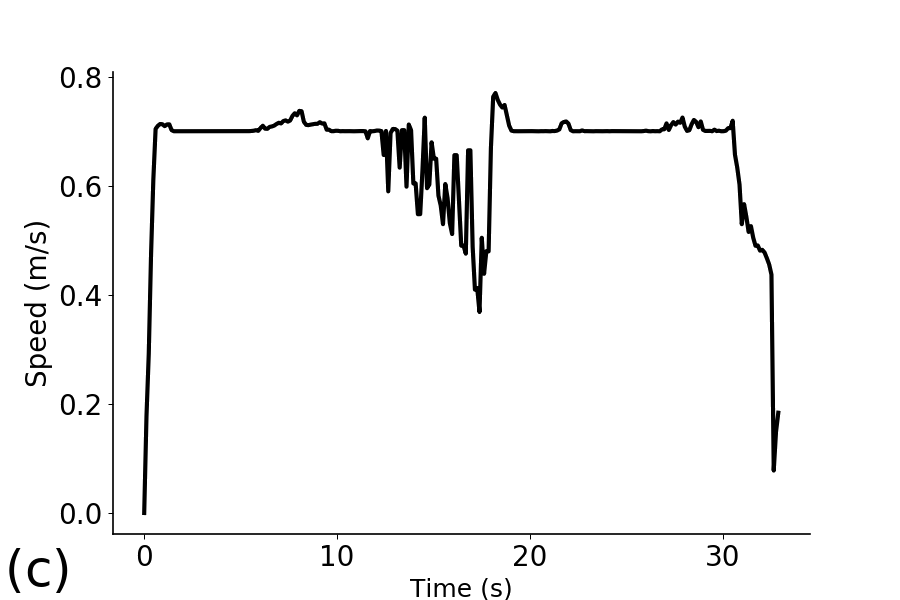
\includegraphics[width=0.9\textwidth]{images/chapter5/vel_corridor_new.png}
%   \caption{Speed: Many openings corridor}
\end{subfigure}
\hspace{-0.17cm}
\begin{subfigure}{0.45\columnwidth}
  \centering
  % include second image
  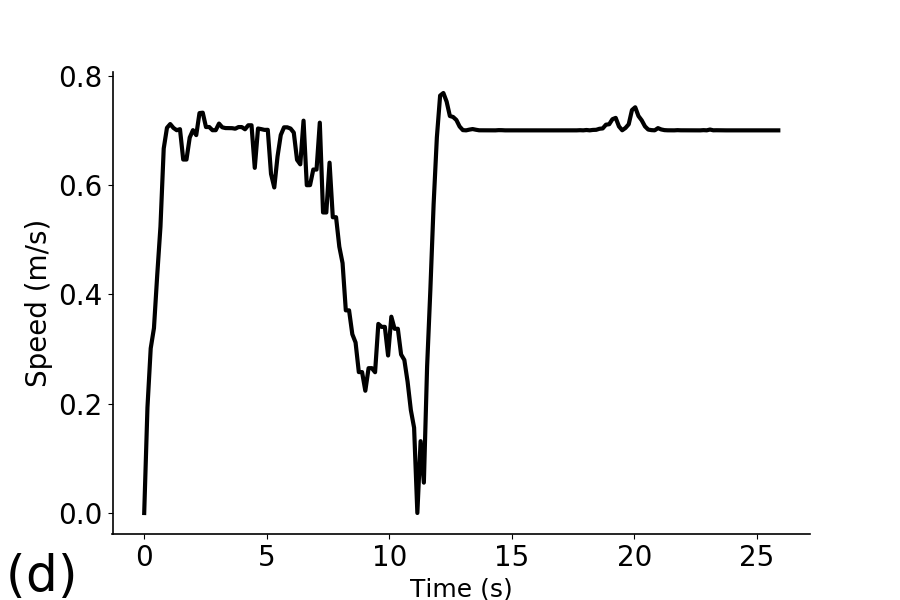
\includegraphics[width=0.9\textwidth]{images/chapter5/vel_pillar_new.png} 
%   \caption{Speed: Pillar corridor}
\end{subfigure}
\caption{Paths and speeds profiles of the robot in corridor scenarios. (a), (c) correspond to the corridor with many openings. (b), (d) correspond to the pillar corridor. The color of the paths indicates the time and progress of the robot, from blue (start) to red (goal).}
\label{fig:corridors}
\end{figure} 
In the case of the corridor with many openings, the robot anticipates that a human might emerge anytime and tries to move away from the openings. However, when it sees a human passing through the corridor, it tries to provide more space to the human by moving to one side. At the same instance, it faces the forces from the \textit{invisible humans} and tries to find a balance between these and the visible human. By observing the path and speed profile of this scenario from Fig. \ref{fig:corridors} (a) and (c), we can see that the robot moves away as well as reduces its speed rapidly to accommodate the visible human. Nonetheless, it does not move very close to the door as it anticipates a human emergence. 
 
In the corridor with pillars, the robot faces another complex situation where it has to pass through a very narrow opening and has to let the human pass through the same as shown in Fig. \ref{fig:corridor_scene} (b). From the path and speed profiles of this scenario from Fig. \ref{fig:corridors} (b) and (d), we can see that the robot slows down rapidly while moving to a side and momentarily stops before moving forward again. Here, the robot stops and lets the visible human pass before it can continue its navigation. Further, it detects the narrow passage scenario discussed in section~\ref{psg_detect} and changes to \textbf{Pass Through} mode. We can, therefore, infer that \acrshort{cohan} always tries to find a fine balance between visible and \textit{invisible humans} and can mitigate very complex situations.
 
\subsection{Testing the Accuracy and Robustness}
\begin{figure}[h!]
\centering
\begin{subfigure}[t]{0.45\columnwidth}
  \centering
  % include first image
  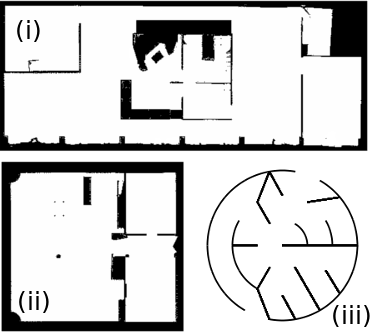
\includegraphics[width=0.8\textwidth]{images/chapter5/maps.png}
  \caption{Maps used for testing (i) LAAS (ii) Bremen (iii) Random Maze}
\end{subfigure}
\hspace{-0.17cm}
\begin{subfigure}[t]{0.45\columnwidth}
%   \centering
  % include second image
  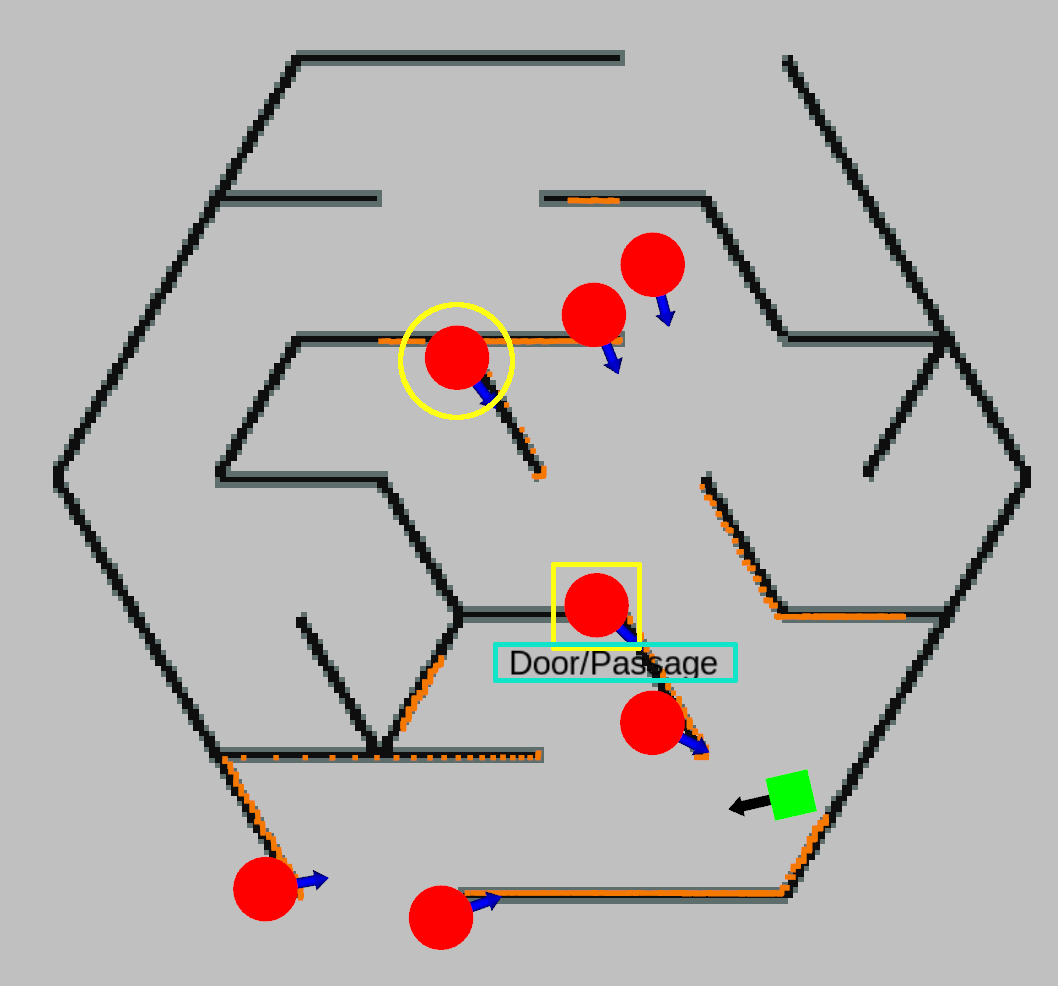
\includegraphics[width=0.9\textwidth]{images/chapter5/passage_detect_fail.png} 
  \caption{Failed detections}
\end{subfigure}
\caption{(a) Different maps used for testing the robustness and accuracy of the approach. The map in (iii) shows an example of randomly generated maze. The other maps are standard ones. (b) Different types of failed detections. The detection in yellow circle is a false positive whereas that in yellow square is an overlap (possibly true). The passage detection is also wrong as the wall is detected as passage. The green cube with black arrow shows the robot and its direction. The red cylinders are the \textit{invisible humans}.}
\label{fig:random_exps}
\end{figure}

\noindent For testing the proposed algorithm, we have designed randomised experiments. We either generate a random map using the Maze Generator\footnote{\url{https://github.com/razimantv/mazegenerator}} or randomise the position of the robot in the known map. The maps used for these experiments are shown in Fig. \ref{fig:random_exps} (a). The LAAS and Bremen maps are collected from the models of real spaces. Fig. \ref{fig:random_exps} (a) (iii) shows a random map generated using the Maze Generator. Fig. \ref{fig:random_exps} (b) shows some failed detections using the proposed algorithm that are taken care of while calculating the accuracy. The red circles with blue arrows are the predicted \textit{invisible humans}. The invisible human in the yellow circle is classified as a false positive, as no human could be located inside the wall. The detection in the yellow square is similar, but it is not completely inside the wall. We call this case an `overlap' and classify this also as a false positive. The door/passage detected (cyan rectangle) in this picture is wrong, and we classify this as a false positive while calculating accuracy for passage detection. The green square with the black arrow is the robot in the figure.

\subsubsection{Robustness and Accuracy }
To test the robustness of the proposed algorithm, we perform several randomised experiments in different settings. In the LAAS and Bremen maps, we randomise the position of the robot and evaluate the detections manually. We did 50 such evaluations for each of the above two maps. In the next set of experiments, we generate a random map and place the robot in a random pose and then evaluate the detections. In this case, we have done 100 evaluations using 100 randomly generated maps. The calculated accuracy of our \textit{invisible humans} detection algorithm based on these 200 experiments is $76.85\%$. However, if we include the overlaps as true detections, it increases by over $12\%$ to $89.16\%$. These overlaps could be reduced by improving the filtering. Table \ref{acc} shows the list of experiments and the accuracy in each case.
\begin{table}[h!]
    \centering
    \begin{tabular}{|c|c|c|}
    \hline
    & \multicolumn{2}{c|}{Invisible Humans Detection}\\
    \cline{2-3}
    Experiment & \textit{Accuracy ($\%$)}& \textit{Accuracy with overlap ($\%$)} \\
    \hline
    \textit{LAAS} & 91.82 & 94.55\\
    \hline
    \textit{Bremen} & 65.28 & 81.94 \\
    \hline
    \textit{Random} & 76.90 & 90.42 \\
    \hline
     \textbf{Overall} & \textbf{76.85} & \textbf{89.16} \\
    \hline
    \end{tabular}
    \caption{Accuracy calculated based on 200 experiments in 3 different environments. By correcting the overlapping detections, the accuracy could be increased by over $12\%$.}
    \label{acc}
\end{table}
% \vspace{-0.5cm}

For calculating the accuracy of passage detection, we have performed similar experiments and evaluated the detections in 200 experiments. Here, we classify the detection simply as either true or false. There are also cases where there are no detections. In such cases, no detection within limits is classified as false, and the out-of-the-limits is classified as a miss. Table \ref{acc_pass} shows the accuracy of passage detection in different settings. The overall accuracy based on these experiments is around $62.50\%$. Note that the percentage of misses is around $23.50\%$. They can be eliminated by having higher or adaptive detection limits. The limits have to be set based on the requirement.
\begin{table}[h!]
    \centering
    \begin{tabular}{|c|c|c|}
    \hline
    & \multicolumn{2}{c|}{Passage Detection}\\
    \cline{2-3}
    Experiment & \textit{Accuracy ($\%$)}& \textit{Misses due to limits ($\%$)} \\
    \hline
    \textit{LAAS} & 66.00 & 30.00 \\
    \hline
    \textit{Bremen} & 54.00 & 36.00 \\
    \hline
    \textit{Random} & 65.00 & 14.0 \\
    \hline
     \textbf{Overall} & \textbf{62.50} & \textbf{23.50} \\
    \hline
    \end{tabular}
    \caption{Accuracy calculated based on 200 experiments in 3 different environments. Increasing the limits of detection could increase the accuracy by over $23\%$. These limits could be decided based on the requirement.}
    \label{acc_pass}
\end{table}

\section{Real-World Tests}\label{real_chap5}
The \acrshort{cohan} system is installed on the PR2 robot in our lab and then tested in the doorway scenario discussed above. In these experiments, we do not use any human tracking as these are tests for \textit{invisible humans}. The localisation of the robot is done using the \textit{amcl} localization\footnote{\url{http://wiki.ros.org/amcl}} package in ROS. The system runs entirely on the robot and only the goals were given from a remote computer.
\begin{figure}[h!]
    \centering
    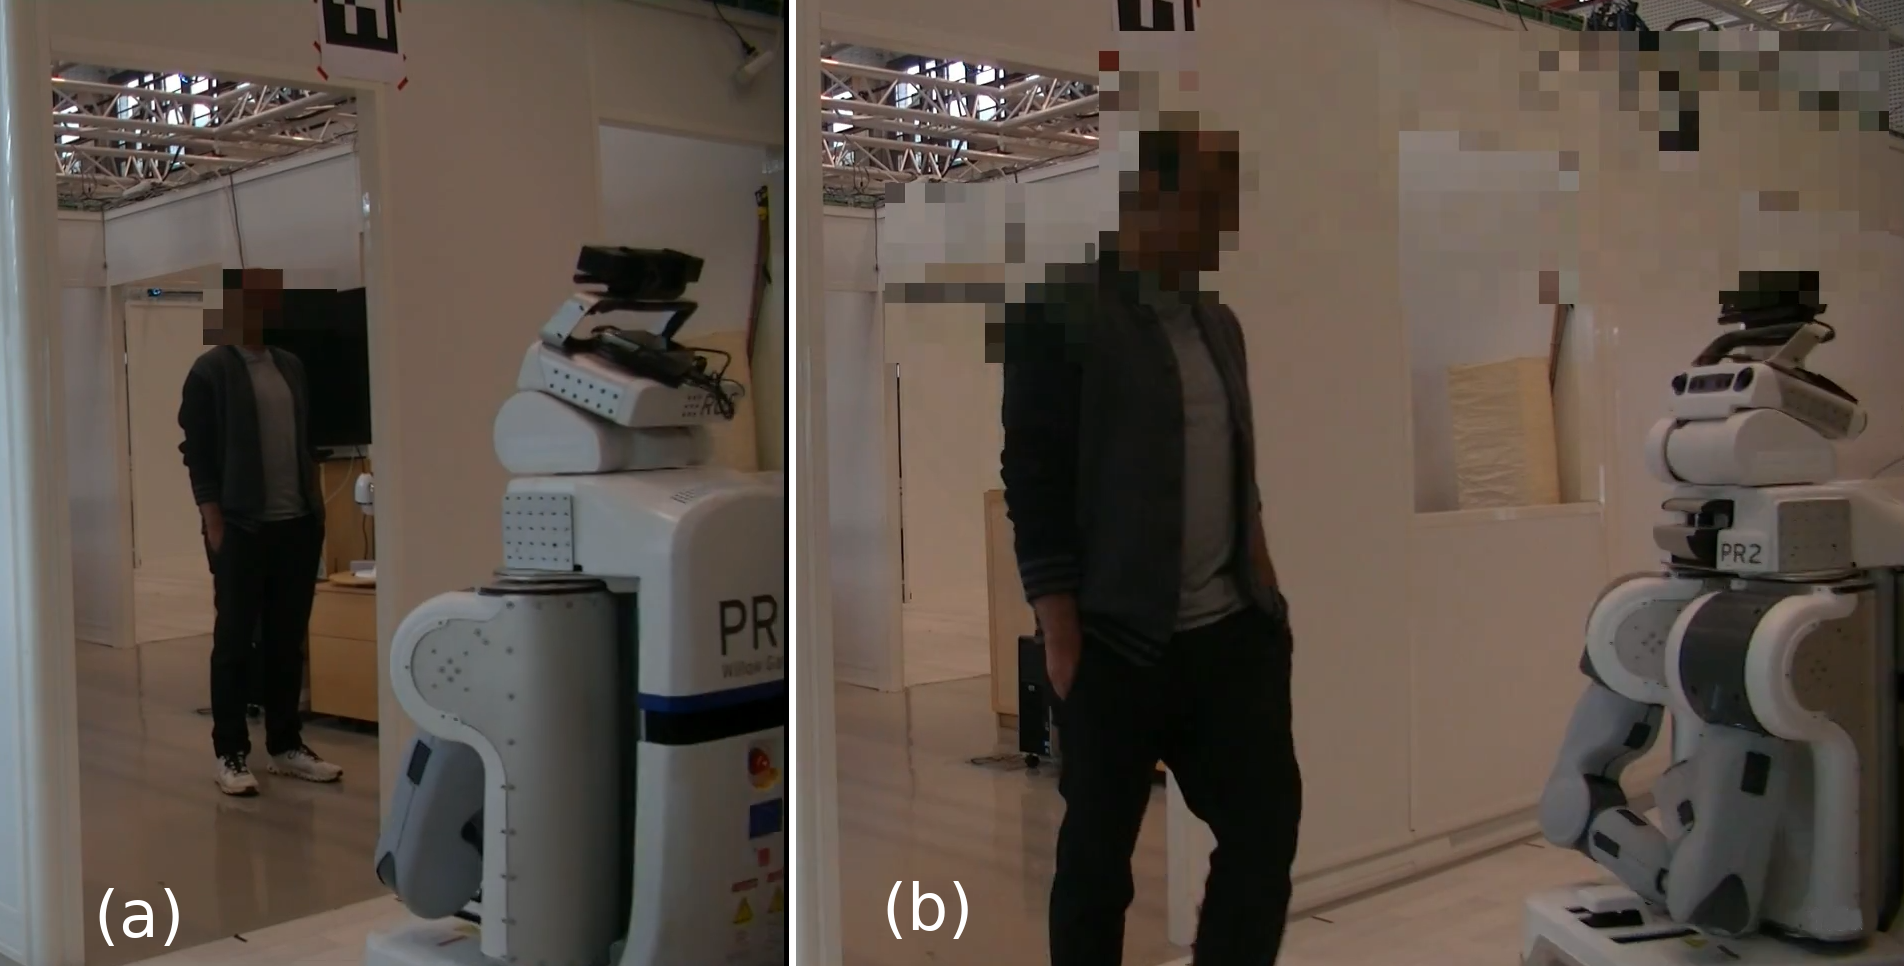
\includegraphics[width=0.9\columnwidth]{images/chapter5/real_video}
    \caption{Real world experiment setting (a) Human is inside the room and does not move. (b) The human starts coming out of the door as the robot approaches the door. In both scenarios, the robot tries to pass through the door.}
    \label{fig:real_photo}
\end{figure}

We performed two kinds of experiments around the door, as shown in Fig. \ref{fig:real_photo}. In the first situation, shown in Fig. \ref{fig:real_photo} (a), the human remains stationary, whereas in the second situation, shown in Fig. \ref{fig:real_photo} (b), he comes out of the door as the robot approaches the door. The first situation is tested, with and without the \textit{invisible humans} constraint, and the results are shown in Fig. \ref{fig:real_plots}. We can see from the figure that the real-world results match the results of the simulation approximately both in the paths and the speed profiles. The robot takes a larger turn and aligns itself with the door before moving towards the entrance. The video\footnote{\url{https://youtu.be/cbeFRkEdGgA}} clearly shows the effect of the added constraint as well as the shift to the new modality \textbf{Pass Through}. Note that in Fig. \ref{fig:real_plots} (c), the robot halts momentarily. This may be because of a sudden human appearance or moving very close to the wall.

\begin{figure}[h!]
    \centering
    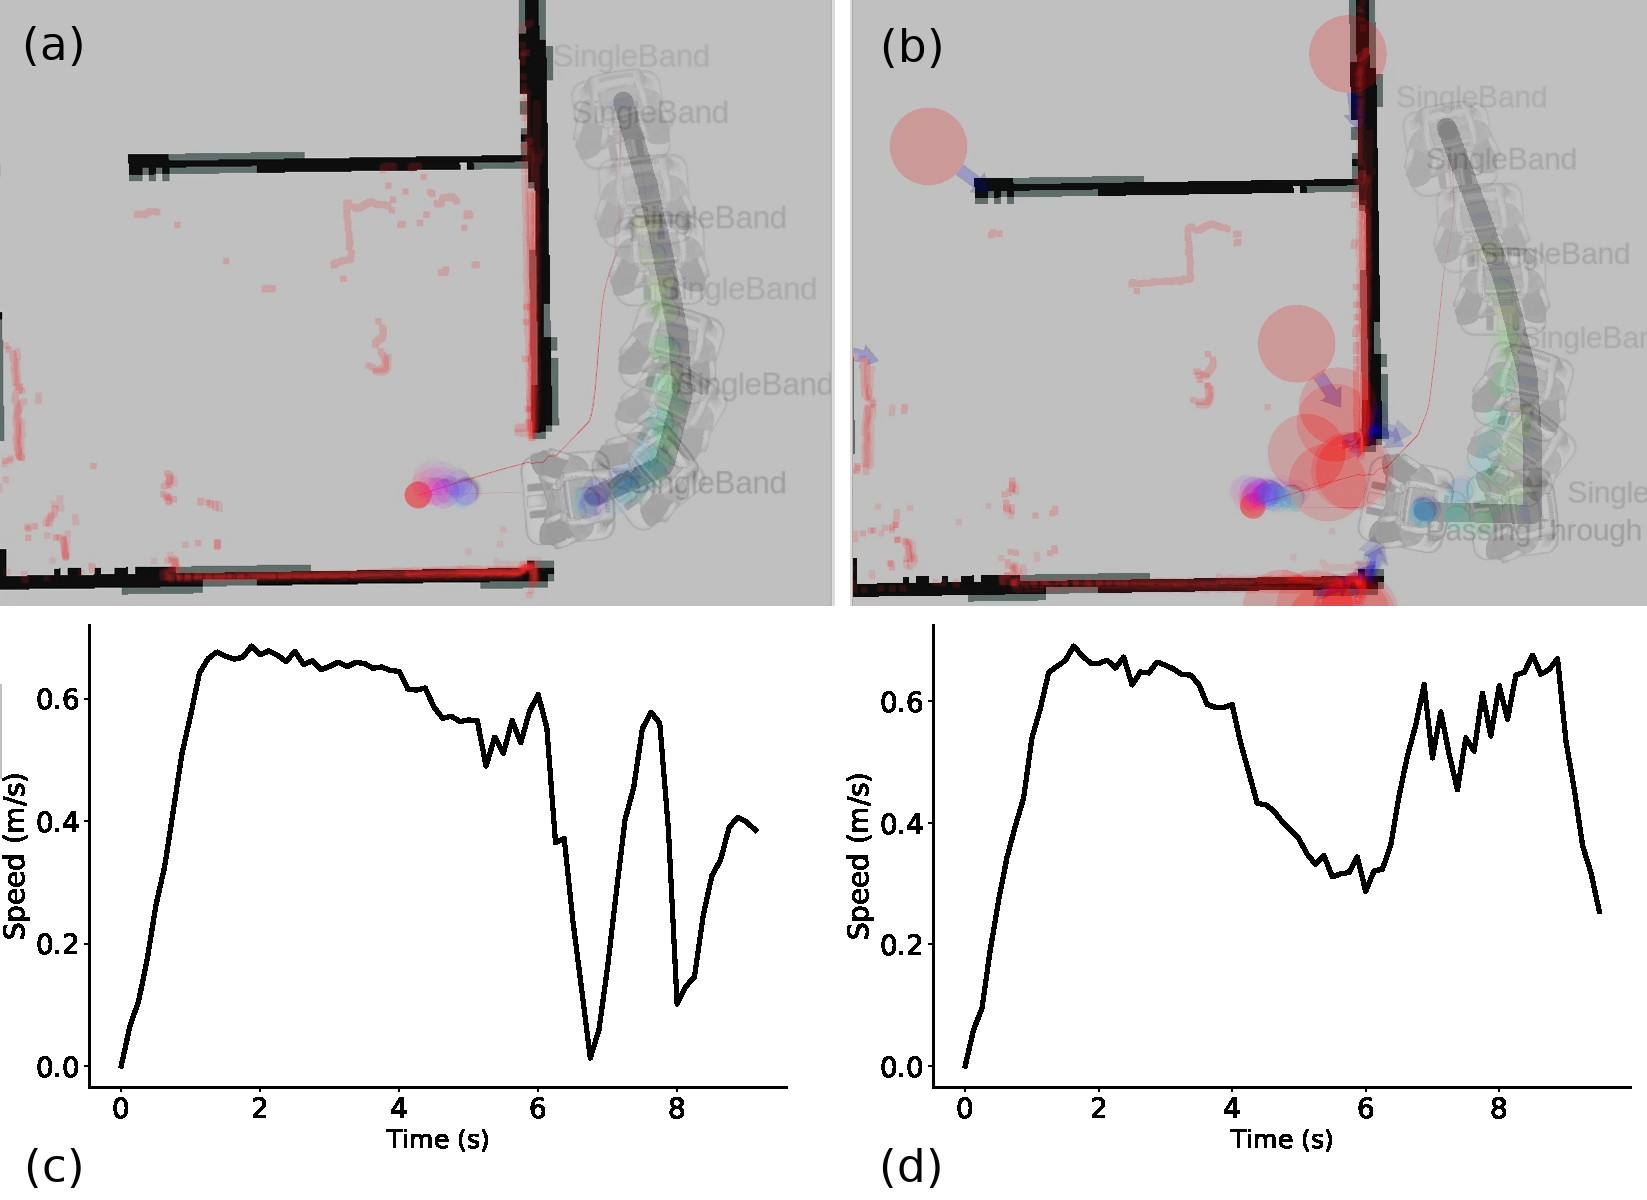
\includegraphics[width=0.9\columnwidth]{images/chapter5/real_compare_new}
    \caption{Paths and speed profiles without (a, c) and with (b, d) \textit{invisible humans} constraint. The addition of the constraints makes robot takes larger turn (b).}
    \label{fig:real_plots}
\end{figure}
\begin{figure}[h!]
\centering
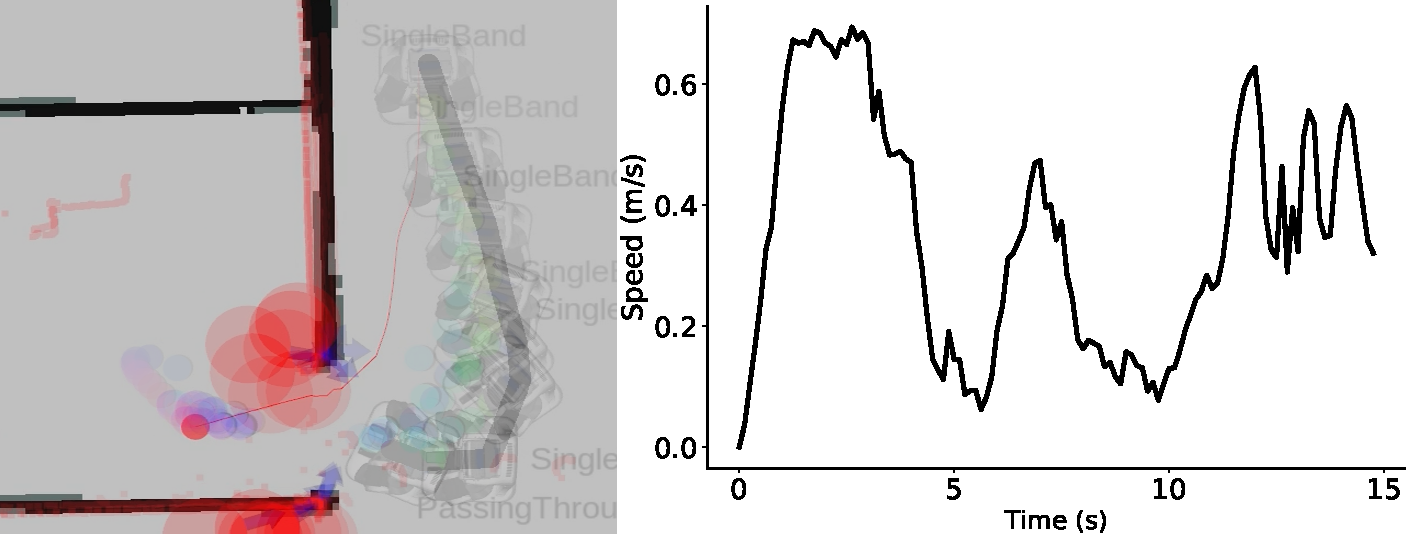
\includegraphics[width=0.9\columnwidth]{images/chapter5/move_final_fig.png}
\caption{Path and speed profile in the sudden emergence scenario.}
\label{fig:real_move_plots}
\end{figure} 

The second situation is similar to the sudden emergence scenario, and the results of this run are shown in Fig. \ref{fig:real_move_plots}. The human emerges out of the door as the robot starts to move towards it. However, thanks to the \textit{invisible humans} constraint, the robot is not very close to the door and leaves enough space for the human to pass through. In this scenario, the robot slows down twice, once when the human emerges and then to align itself with the door. 

\section{Discussion and Limitations}\label{discussion_chap5}
The introduction of \textit{invisible humans} into human-aware navigation planning is relatively new and requires further research. We present one possible approach to address this issue. What is particularly interesting here is that our approach is modelled as a situation assessment and prediction ability to integrate into a mobile robot human-aware navigation. Having this, we can have a robot that can interact, using several modalities, with humans present in its field of view while making provisions to adapt to humans that are not yet seen. One difficulty we faced was the integration of all these features without being ``too conservative'' and avoiding another case of the ``freezing'' robot. However, there are still some limitations to this approach. Since the approach is based on a 2D map, we can have false detections in the regions visible through the head of the robot but not through the base. There may also be some false detections in complex maps. Both these can be mitigated by augmenting the current approach with new sensor data and filtering further.

\section{Conclusion}\label{conclude_chap5}
We have proposed an approach to estimate the locations of \textit{invisible humans} on a 2D map. These \textit{invisible humans} are then integrated into our human-aware navigation planner via a new constraint. We have also shown how narrow passages can be identified by exploiting the detected \textit{invisible humans}. We have presented the qualitative analysis of several simulated scenarios, followed by the results of accuracy and comparisons with some planners. Finally, we have shown the real-world experiments and presented some discussion. In the future, we plan to refine this approach further and address the different modalities identified in a better manner. We also aim to build a complete human-aware navigation system that can address very intricate human-robot interactions.

% These real world demonstrations again prove the necessity of the proposed concept in HAN.



% \ifdefined\included
\else
\setcounter{chapter}{5} %% Numéro du chapitre précédent ;)
\dominitoc
\faketableofcontents
\fi

\chapter{InHuS}
\chaptermark{InHuS}
\label{chap:6}
\minitoc

\section{Introduction}
Vers simulation humain intelligent pour benchmarker planner robot (nav + tache)
InHuS:
ère du digital twin : 1er pas vers ça, un peu générique, fait pour nav mais pourrait aller plus loin
A mettre dans un chapitre "a part"

Objectives - Current challenges in testing ha nav

\section{Related work}


\section{Description}
architecture and how it works

\subsection{main components}
\subsection{attitudes}
\subsection{metrics and logs}

\section{Main results}
able to numerically identify the HA behavior of CoHAN w/r SMB)


\section{Extension: IMHuS}

\subsection{Describe}
\subsection{results?}

\section{Discussion and Limitations}
\section{Conclusion}
% \chapter{Conclusions}
% \addstarredchapter{Conclusions} 
\markboth{Conclusions}{}

% The final remarks, lessons learnt, and future perspectives are discussed in the Conclusions chapter. The supportive work presented in Appendix A shows how an intelligent human agent is developed for the case of HAN. Further, different methodologies employed to simulate human agents for testing our HAN system are also presented. Throughout this thesis, whenever we refer to robot navigation, it is always a mobile robot with either differential or omnidirectional drive navigating on a 2D plane.

%%%%%Update this later%%%%%%%%%%%%%

In this thesis, we have explored the problem of mobile robot navigation in human environments, generally called human-aware navigation (HAN). We have presented detailed literature on how the field evolved and some existing challenges. Numerous solutions were proposed for HAN in motion planning literature by modelling humans as special obstacles. However, we believe that HAN is essentially an interaction between humans and robots. Therefore, it should satisfy the principles of HRI. In this thesis, we have put together these ideas and proposed a HAN that assesses a situation to take appropriate action. Although situation assessment and behaviour shifting have already been explored in HAN, they were mostly used on top of motion planning systems. Unlike the previous approaches, we have introduced situation assessment at the level of trajectory planning to shift between different modes of planning while the robot navigates to the goal. As this low-level mode shifting was combined with proactive planning, the robot can deal with complex situations in an efficient manner before it is too late. Proactive planning itself has some very interesting features, like quick plan adaptations and early intention shows, but there could be some very complicated situations where proactive planning may not be sufficient. The situation assessment based modality shifting is useful in such places.

We have presented three versions of our HAN system, starting with the idea of introducing modality switching inside the local trajectory planner. There were several improvements over the previous version of HATEB, and these improvements, combined with the mode switching scheme, are some of the major contributions of this thesis. Qualitative and quantitative results have shown the advantages of such an approach in various settings. We then moved on to propose a Human-Aware Navigation Stack called CoHAN with many changes to scale the system to multiple humans and to address different types of humans. CoHAN can be seen as a complete navigation stack for HAN with different costmap layers, human path prediction mechanisms, and several modes of planning that can solve most of the intricate human-robot navigation scenarios. The early intention show and the Backoff-recovery act as implicit communication mechanisms to tell the human what the robot is going to do. In the future, we plan to integrate more explicit communication through head orientation and probably voice. Various kinds of human states combined with the situation assessment can address more complicated scenarios, and to ease this, we plan to modularize the future version of CoHAN with detailed documentation. CoHAN has been tested on simulated crowds and has already shown some promising results. However, we believe that crowd navigation could be more complex, and we need more modalities and mechanisms to handle crowds efficiently. We have already presented some ideas we plan to integrate into the future version, and we expect to add more.

Apart from addressing multi-context navigation, we have also focused on one key aspect throughout the development of our HAN system, legibility. We have introduced some new human-aware constraints to make the robot's motion more legible to the human. To show the intention of the robot early, we have proposed TTC, TTCplus and Relative Velocity constraints. The Relative Velocity constraint also addresses the issue of directionality in the crossing or close-to-human navigation scenarios. We have introduced the Visibility constraint to avoid any surprises or shocks to a human when the robot overtakes the human. One more attempt to improve legibility was done through 'invisible humans’. We have introduced this concept into HAN to make sure that the robot is aware not only of the humans it is seeing but also of the environment and the places humans might emerge. We believe that this makes the system more complete and ready to face any kind of environment without behaving erratically or freezing. The `invisible humans’ concept has also made it possible to identify different places on the map through geometric reasoning and introduce different modalities of planning depending on the situation. Further, the algorithm was rigorously tested and showed satisfying performance in some very complex maps. The final version of CoHAN integrated with the `invisible humans’ has been shown to perform better and move smoothly without having any freezing robot problems. 

One of the open challenges in HAN is its evaluation, and the currently existing metrics do not do justice while the robot is navigating very dense crowds or confined spaces. As most of them are based on proxemic zones that are variable from place to place and the experiences of the person, it makes it more difficult to generalise the metrics to all cases of HAN. Therefore, we proposed some new metrics of evaluation using velocities and visibility along with distance. The velocity based metrics, $cost_{danger}$ and $cost_{passby}$, aim to measure the feeling of threat and discomfort caused to the human depending on the direction and speed of the robot's heading. Since these metrics combine distance and velocity, they can explain intricate settings better than proxemic zone violations. The first one of the vision based metrics,$cost_{visibility}$, was designed to measure how well a robot can approach a human from behind. The other metrics, $cost_{surprise}$ and $cost_{react}$, aim to measure the surprise(or shock) and risk caused when a robot appears in front of a human suddenly. The comparison between a standard navigation planner and a HAN planner showed how these metrics evaluate the `human awareness' of the system.

%%%%%%%%%%Talk about the magic numbers %%%%%%%%%%%

Human-aware navigation is not a very simple problem to address, and it taught us some valuable lessons. The developed systems are hard to validate in real-world settings. The experiments could be tedious, not easily reproducible and can be limited. Not every robot is the same. The structure of the robot matters to humans in the environment. Their behaviour towards the robot changes as the shapes and designs of the robot change. Humanoid structures are accepted better than simple mobile bases, even with the same algorithm. One of the important aspects while developing a HAN system is to have a good simulator that can generate realistic human behaviours. To this date, there is no perfect human simulator. The HAN research community has been using crowd simulators or directly testing with real humans. Crowd simulators are mostly reactive and are not realistic. On the other hand, tests with real humans are tedious and require a lot of resources and time. Although there is rapid growth in this aspect, the community is still waiting for a reliable robot simulator that can simulate rational human agents. We require more user studies to understand the intricacies of human-robot navigation. This is the right moment to invest more time into these studies, as drones and autonomous vehicles have also entered the field. The robotics community seems to have realised this, and now, there are special sessions dedicated to human-aware motion planning and human-aware navigation. The number of studies has already increased, and many researchers in motion planning are coming together to address this complicated yet interesting problem of robotics that can eventually lead to a society where humans and robots coexist.

There are already many immediate future perspectives for HAN. As autonomous vehicles have already hit the roads, it is time to make them behave socially by making them aware of humans and their intentions. An autonomous vehicle not only needs to be safe but also needs to obey certain rules and untold norms followed in society. HAN studies this problem exactly. Drones have become very affordable, and some companies are planning on using them for deliveries, while others are planning to use them as helpers in construction. All these applications require drones to navigate around humans and communicate with them. HAN in drones needs to study these in more detail and come up with better navigation systems for drones. Apart from guiding people in public places, some other applications of HAN  lie within warehouses where they need to work or deliver goods to different locations. These environments are more structured, and solving HAN in such places is much easier. HAN has been and will always be used in the sector of service robotics. Be it a robotic companion, a robotic wheelchair or robots in hospitals delivering medicines or equipment the HAN system faces dynamically changing environments where safety is one of the main concerns. A multi-context tunable navigation system could address most of these scenarios by choosing a set of parameters suitable for the setting.



% \appendix
% \chapter{Simulating Human Agents for Testing HAN}
One of the challenges during the development of a HAN system is to test the system before its final deployment and real-world runs. Robotic simulators are of great use during this period as we can test the system under various conditions and in several environments. Unlike the classical setting, testing HAN requires the simulation of humans, which is still research under development. Until recently, the HAN community used the crowd simulators like Pedsim or MengeROS~\cite{aroor2017mengeros} to simulate humans in semi-crowded or crowded scenarios. However, the motion generated by these simulators uses reactive schemes like \acrshort{sfm} or \acrshort{orca}, which are good for generating crowds but lack intelligence at the level of an individual human. Recent simulators like SEAN~\cite{tsoi2020sean, tsoi2022sean} and SocNavBench~\cite{biswas2022socnavbench} tried to generate somewhat intelligent behaviours using new approaches and real-world data. However, these human agents are either not reactive (as they replay real-world trajectories without considering the robot) or use schemes similar to \acrshort{orca}. Although they have better human agents and environments for testing HAN, they still lack intelligent agents that can be used to test intricate scenarios in spaces like offices, labs or homes. Hence, we have used different ways to control the human(s) while testing the HAN proposed in this thesis. These ways include manual control using a joystick, a simple human controller that follows the generated trajectories, and finally, an intelligent human with rational decision-making capabilities.      

\section{Planning and Control for Human Agents}
In this section, we talk about the simple modes and planners employed to control the human avatar in the robot simulator. A human is assumed to be a robot with special requirements.

\subsection{Manual Control}
One of the simplest ways to control a human is to move the human manually using a keyboard or joystick. This is efficient in testing some very complicated scenarios involving intelligent decisions. Since a real human is already controlling the human avatar in the simulator, all the decision-making process is handled by the human operator. To integrate such human avatar into our system, we used the \textbf{\textit{joy}}\footnote{\url{http://wiki.ros.org/joy}} \acrshort{ros} package and then mapped the inputs of the joystick to the avatar's velocity with a cap at \SI[per-mode=symbol]{2}{\metre\per\second}.

Manual control is good for testing some interesting and particular cases, but it becomes tiresome to run several scenarios to benchmark or quantify the results. Moreover, the simulation runs cannot be completely automated as the human operator is always involved in the loop. So, the next solution was to plan and control the human, like the robot. It is different from collision avoidance algorithms as the human has a global path to trace and a separate local planner to move the human. 

\subsection{Planning based Control}
To automate and replicate the tasks easily, we have developed a simple \textbf{\textit{humans navigation}}\footnote{\url{https://github.com/sphanit/humans_nav}} package using the \textbf{\textit{global planner}}\footnote{\url{http://wiki.ros.org/global_planner}} in \acrshort{ros} and a simple controller. The developed system has two modes of operation:
\begin{enumerate}
    \item \textit{Trajectory following}: In this mode, the human follows the trajectory that is provided externally through a \acrshort{ros} topic. We used this mode to test the ideal situations where the human follows the trajectory planned by \acrshort{cohan}.
    \item \textit{Goal-based Control}: This mode is more autonomous as we only provide a goal via a \acrshort{ros} topic, and the system plans and moves the human to the goal. The planning module updates the plan as the human moves, and the simple controller traces the path. This mode was used to run multiple tests to check how well the robot adapts to the human.
\end{enumerate}
Both these modes can control more than one human simultaneously. The \textit{Trajectory Following} mode used the trajectories planned by \acrshort{cohan} to move the humans. The trajectory provided the desired velocities, which were sent directly to the human controller. However, in the \textit{Goal-based Control} mode, the velocities were calculated based on the current position and planned paths of the humans. To accept multiple goals and plan for all the humans together, a \textbf{\textit{multi-goal planner}} was developed, and it is used internally by the \textbf{\textit{humans navigation}} package to get plans based on the provided goals.

Even though this kind of system solves the issues of automation and is less tiresome to the developer, the human agent is still not intelligent and simply follows the given trajectory. Although the trajectory provided by \acrshort{cohan} takes care of many human-robot social constraints, this ideal behaviour may not be expected from humans. In the second mode of control, the human agent might have better behaviour, but the agent is still not intelligent and somewhat reactive, like in collision avoidance schemes. 

\section{InHuS}
InHuS\footnote{\url{https://github.com/AnthonyFavier/InHuS_Social_Navigation}}~\cite{favier2022_hri} stands for \textbf{I}ntelligent \textbf{Hu}man \textbf{S}imulator, and it was developed to specifically simulate a human agent that is rational and persistent about its goal, unlike the reactive schemes. 
\begin{figure}[!hb]
    \centering
    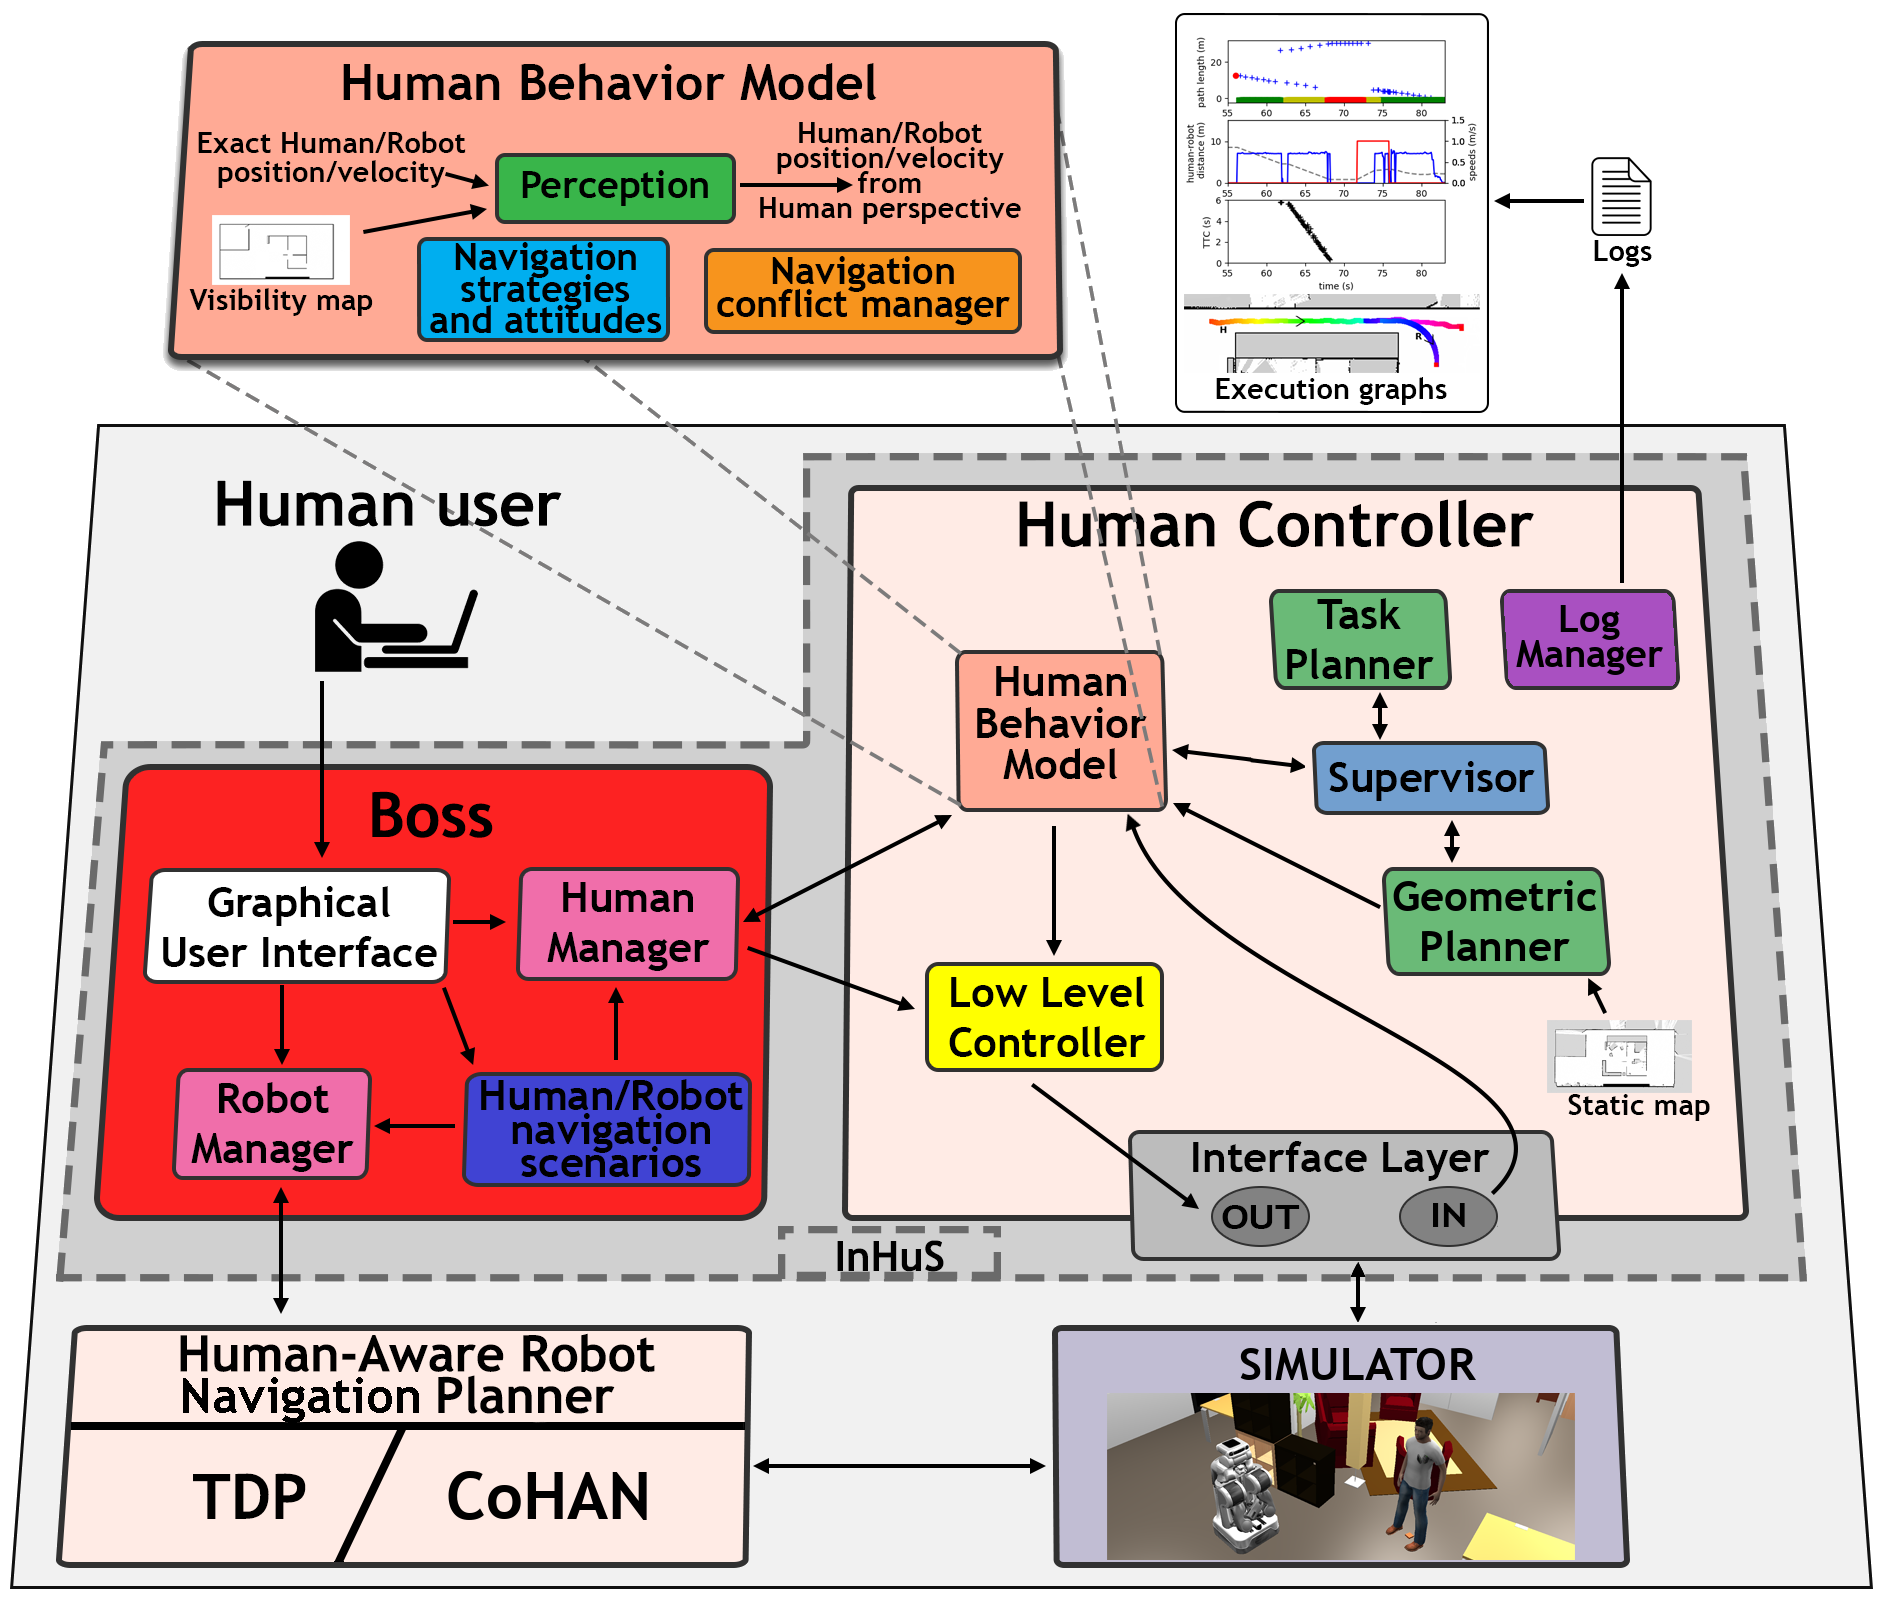
\includegraphics[width=0.9\columnwidth]{images/appendix/architecture.pdf}
    \caption{InHuS Architecture. The system consists of the Boss and the InHuS Human Controller macro components. The human operator interacts with the system through the Boss which in turn interacts with the Human Controller and the HAN Planner. Both the human and the robot controllers are connected to the same simulator where they control different components but share the same environment.}
    \label{fig:inhus}
\end{figure}
\subsection{Architecture}
The architecture of the proposed system is shown in Fig.~\ref{fig:inhus}. InHuS is composed of two major components namely, 1) \textit{Boss} and 2) \textit{Human Controller}. These components are explained in detail below:
\begin{itemize}[label={}]
    \item \textbf{Boss}: The \textit{Boss} component is responsible for taking input from the user and sending the appropriate instructions to the human and the robot planners. Hence it is provided with a graphical user interface through which a user can give individual goals to each agent, run or re-run predefined scenarios or initiate an endless loop of the human and robot navigating continuously from one goal to another. The endless loop can be used to identify the limits of the HAN system under test. After taking the input from the user, this component communicates the navigation goals to the \textit{Robot Manager} and \textit{Human Manager} at the appropriate times. Once the goals are communicated to these components, the \textit{Boss} does not interfere with the execution unless the human operator selects a new goal or scenario.
    \item \textbf{Human Controller}: This is the main component of InHuS that controls human motion and decides what to do in case of a conflict with the robot. It has an internal `\textit{Human Behaviour Model}' that makes these decisions and sets some attitudes to humans. The other major sub-component is the `\textit{Supervisor}', which supervises the execution of the goal and the progress, and activates the respective components as needed. While the `\textit{Geometric Planner}' provides the geometric path and trajectory to the goal, the `\textit{Low Level Controller}' sub-component sends the command velocity to the human avatar. The `\textit{Task Planner}' was used to define different kind of navigation tasks like \textit{go to goal}, \textit{wait} etc. Finally, the \textit{Log Manager} of this component logs the data and sends it to a GUI for visualisation of the calculated metrics.
\end{itemize}

\subsection{Supervisor and Geometric Planner}
The navigation goal of the human avatar is sent to the \textit{Supervisor}, which in turn asks the \textit{Task Planner} for a plan to achieve this goal. The \textit{Supervisor} then supervises and coordinates the execution of all the actions in the plan while managing the conflicts. The navigation plan generally consists of `moving' and `waiting' actions. This kind of architecture allows us to define complex navigation goals with multiple steps. The \textit{Supervisor} queries the \textit{Human Behaviour Model} from time to time to detect any potential conflicts. It has the power to suspend the execution of a plan in case of a conflict and resume it whenever necessary. This is especially useful to execute other actions in case of conflict to show the navigation intention and goal persistence of the human agent, unlike the reactive or simple planning approaches.

When the \textit{Supervisor} has to execute a `moving' action, it sends the navigation goal to the \textit{Geometric Planner}, which generates the path and then calculates the velocity commands to make the human move towards the goal. Depending on the type of trajectory planner selected, human motion can be different. In the current version, the standard \acrshort{ros} Navigation Stack or \acrshort{cohan} can be selected as the \textit{Geometric Planner}. The velocity command given by this component is not directly sent to the human. The \textit{Low Level Controller} receives this velocity and, if necessary, modifies or perturbs this velocity before sending it to the human avatar. This is used to emulate some reactions while navigation called `\textit{Attitudes}', which is presented in the next subsection.

\subsection{Human Behaviour Model}
The \textit{Human Behaviour Model} is the most important component of the proposed architecture. It controls the human avatar and is responsible for the behaviours exhibited by the human agent. As mentioned previously, this component manages the navigation conflicts, and in this version, only the blockage of the path by the robot is handled. Whenever the \textit{Geometric Planner} is called for the first time, the shortest path to the goal without any moving agents is calculated and sent to the `\textit{Navigation Conflict Manager}' of this component. If any blockage of this path by the robot is detected by this component, it changes the human state, and then the \textit{Supervisor} suspends the goal. The human avatar then performs an `approach' action where it moves towards the goal until it reaches a limiting distance from the robot. After this, it stops and waits for the robot to clear the way. Note that any collision avoidance or simple planning strategies will fail to show such behaviour as they will completely change the path of the human agent instead of showing persistence towards the goal.

This component can also set the goals for the human agent apart from the \textit{Boss}. The internal goal selection mechanism is responsible for different \textit{Attitudes} of the human avatar. Three kinds of attitudes are provided in InHuS:
\begin{enumerate}
    \item \textbf{Stop and Look}: It emulates a curious behaviour, where the human avatar navigating to the goal stops and looks at the robot shortly if the robot is in close vicinity of the human avatar. After this action, the navigation to the original goal is resumed.
    \item \textbf{Harass}: This attitude emulates a behaviour where the human avatar continuously disturbs the robot by blocking the robot's path. The idea here is to generate a child-like behaviour for the human avatar.
    \item \textbf{Random Goal}: In this attitude, a new random goal is set to the human avatar while it is already moving towards a goal, emulating something like a change of mind.
\end{enumerate}
To make the system more realistic, this module builds the perception of the human avatar using the map of the environment and the location of the other agents. The information about the other agents is taken directly from the simulator rather than using simulated cameras or lasers. Therefore, the human avatar does not consider the robot that it cannot see, even if it is below the threshold distance geometrically.

\subsection{Logs and Metrics}
The \textit{Log Manager} logs the data of the human-robot navigation interactions and sends it to GUI based data visualiser. This visualiser shows the different states of the human, the paths of the human and the robot, and some metrics to evaluate the robot's navigation. The logged data can also be used to calculate new metrics or methodologies for evaluation. A screenshot of this visualisation is shown in Fig. \ref{fig:gui_inhus}.
\begin{figure}[!ht]
    \centering
    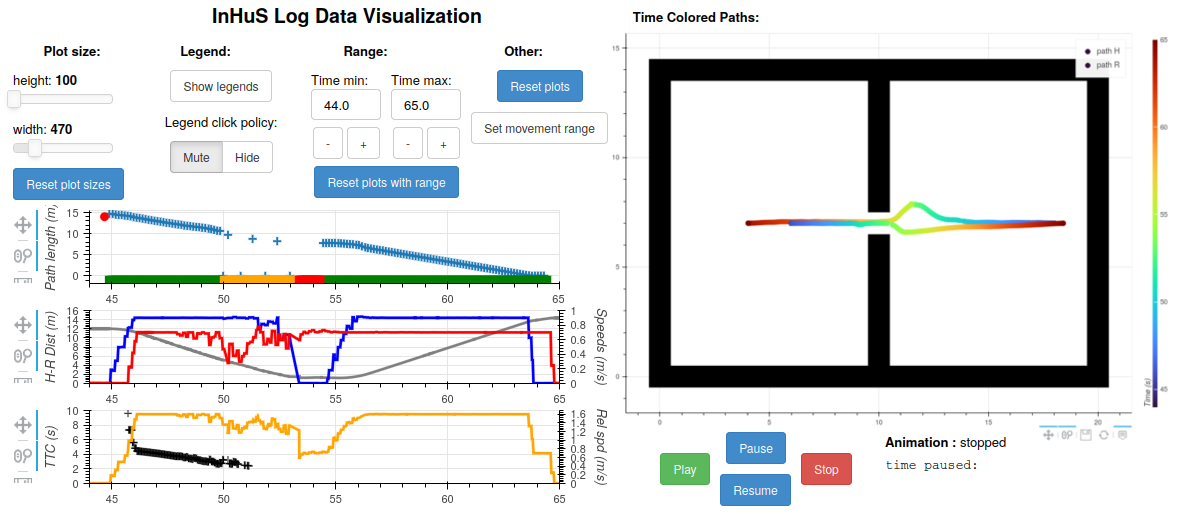
\includegraphics[width=0.9\columnwidth]{images/appendix/gui_bis_bis.png}
    \caption{The data visualisation in GUI. On the right, the paths taken by the agents are shown, while on the left, the human states and the calculated metrics are shown.}
    \label{fig:gui_inhus}
\end{figure}
The paths shown on the right in Fig. \ref{fig:gui_inhus} are coloured over time. It means that the same colour on the paths represents the same time instant, and using this, one can interpret the behaviour of the agents better. On the left, the plot on the top shows the human avatar's distance to the goal and its estimated state over time. If no conflict occurs, the human stays in a single state, and the distance to the goal decreases linearly. The plots below the first one show some of the calculated metrics and the agents' velocities over time. One can calculate and add more metrics as needed using the logged data.

\subsection{Generating Different Behaviours}
\begin{figure}[!h]
    \centering
    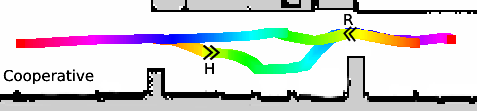
\includegraphics[width=0.9\columnwidth]{images/appendix/paths_coop_new.png}
    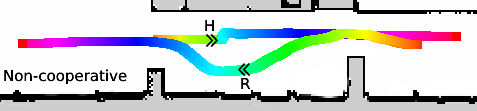
\includegraphics[width=0.9\columnwidth]{images/appendix/paths_stop_new.png}
    \caption{Traversed paths generated by InHuS during the Pillar corridor scenario. The top part is with cooperative settings and the bottom part with non-cooperative settings along with the \textit{Stop and Look} attitude.}
    \label{fig:paths_pillar_corridor_inhus}
\end{figure}
Depending on the \textit{Geometric Planner} and the \textit{Attitude}, different navigation behaviours can be emulated for the human avatar. For example, using the standard \acrshort{ros} Navigation stack and \textbf{Stop and Look} attitude, we can simulate a non-cooperative human who contributes nothing in a setting like a corridor. If \acrshort{cohan} is used, a cooperative yet curious human can be simulated. Moreover, \acrshort{cohan} can be tuned to set a degree of cooperative behaviour. The comparisons of different combinations and behaviours generated are presented in more detail in \cite{favier2021simulating}. Fig. \ref{fig:paths_pillar_corridor_inhus} shows the paths of the robot and human in two situations, one where the human is non-cooperative and curious and the other in which the human is completely cooperative.

% \section{ImHuS}

% \chapter{Effects of Social Constraints}
Each of the proposed social constraints in this thesis has some particular effect on the behaviour of the robot. Some of the predominant effects of these are briefly presented here. Each case presents a scenario without and with the social constraint activated. The figures of each scenario show the paths taken by the human and the robot (starting at blue and moving towards red) and their velocities (robot's velocity in red and human's velocity in blue) below. The velocity plot also includes the distance between the human and the robot during the execution of the scenario. 

\section{TTCplus Constraint}
\subsection{Approach}
\begin{figure}[!htb]
\centering
\begin{subfigure}{0.5\columnwidth}
  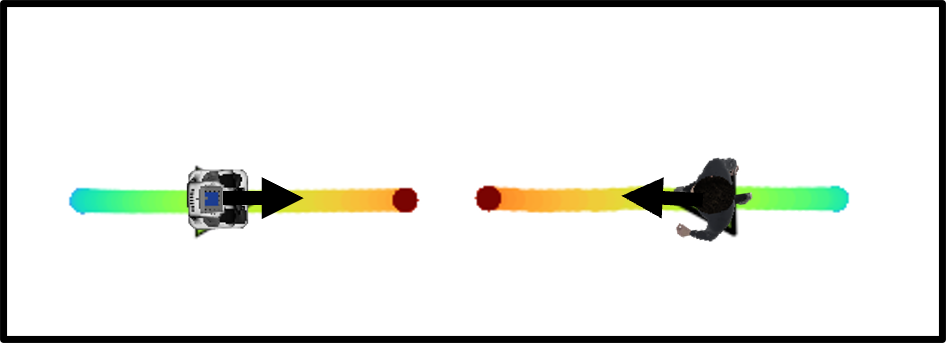
\includegraphics[width=\textwidth]{images/appendix/ttc/approach/approach_without.png}
\end{subfigure}
\vspace{0.5cm}
\begin{subfigure}{0.8\columnwidth}
  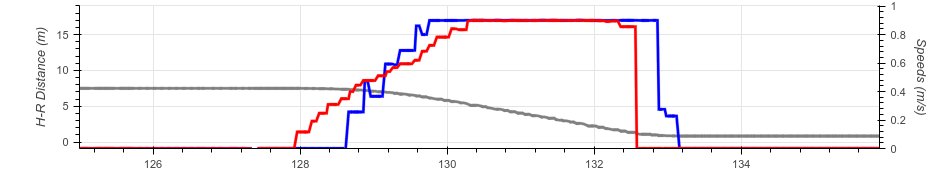
\includegraphics[width=\textwidth]{images/appendix/ttc/approach/without.png}
  \caption{without TTCplus}
\end{subfigure}

\begin{subfigure}{0.5\columnwidth}
  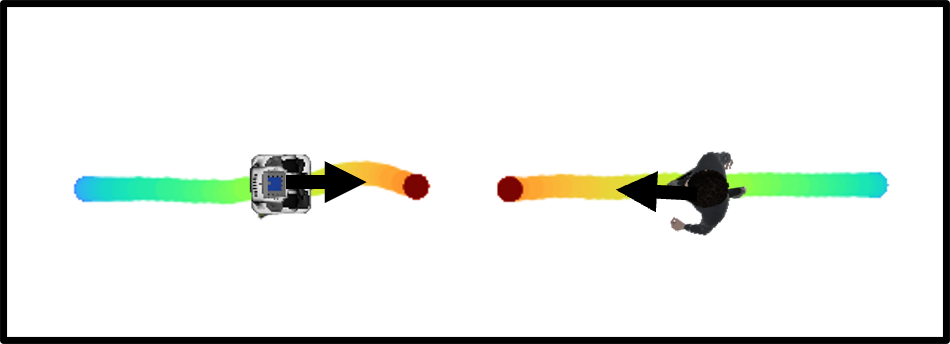
\includegraphics[width=\textwidth]{images/appendix/ttc/approach/approach_with.png}
\end{subfigure}
% \hspace{-0.75cm}
\begin{subfigure}{0.8\columnwidth}
  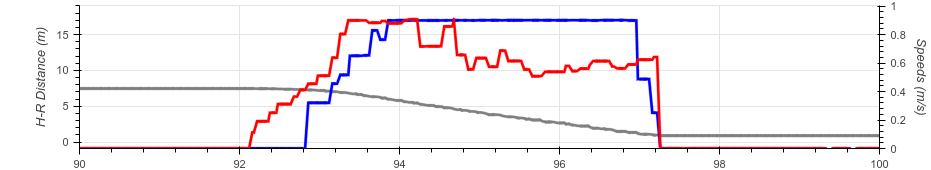
\includegraphics[width=\textwidth]{images/appendix/ttc/approach/with1.png}
  \caption{with TTCplus}
\end{subfigure}
\caption{The robot approaches a human head-on. The addition of the TTCplus constraint makes the robot deviate a little and slow down as it nears the human.}
\label{fig:approach_ttc}
\end{figure} 

In this scenario, the robot and human move towards each other and stop at a very close distance from each other. From Fig.~\ref{fig:approach_ttc} (a), it can be seen that the robot and human move at their full speeds towards each. However, with the addition of the TTCplus constraint, the robot has a decreasing velocity profile as the human-robot distance decreases, showing the robot's intention to stop (shown in Fig.~\ref{fig:approach_ttc} (b)).

\subsection{Open Space Crossing}
\begin{figure}[H]
\centering
\begin{subfigure}{0.5\columnwidth}
  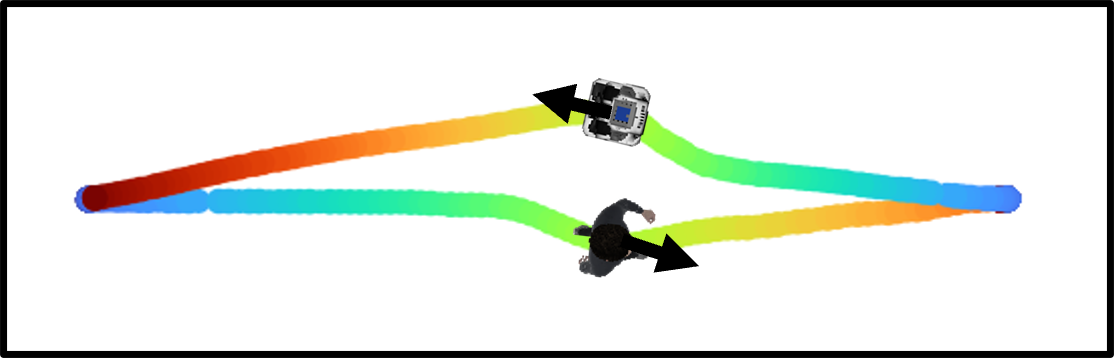
\includegraphics[width=\textwidth]{images/appendix/ttc/wide/without.png}
\end{subfigure}
\vspace{0.5cm}
\begin{subfigure}{0.8\columnwidth}
  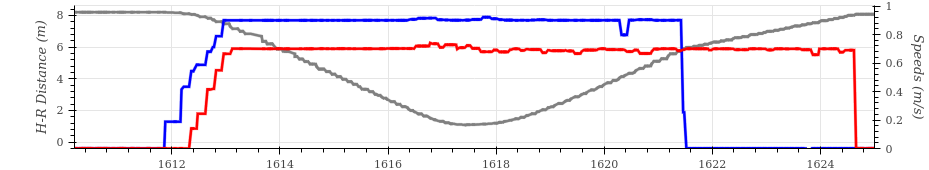
\includegraphics[width=\textwidth]{images/appendix/ttc/wide/wide_without1.png}
  \caption{without}
\end{subfigure}

\begin{subfigure}{0.5\columnwidth}
  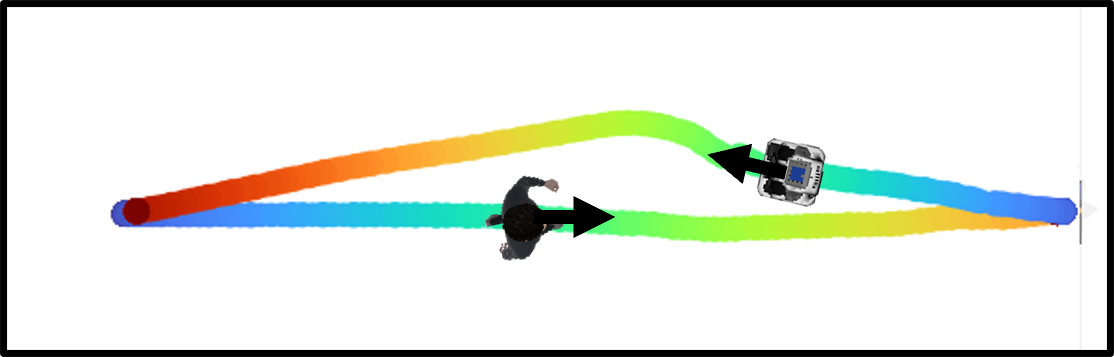
\includegraphics[width=\textwidth]{images/appendix/ttc/wide/with.png}
\end{subfigure}
% \hspace{-0.75cm}
\begin{subfigure}{0.8\columnwidth}
  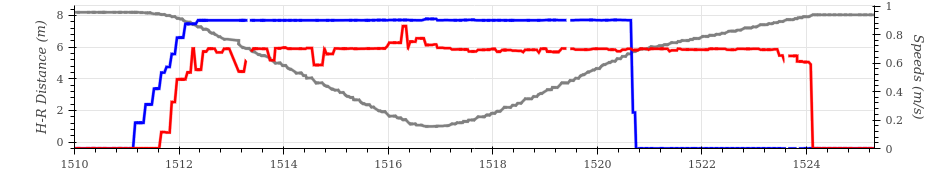
\includegraphics[width=\textwidth]{images/appendix/ttc/wide/wide_with2.png}
  \caption{with}
\end{subfigure}
\caption{The human and the robot cross each other in an open space. The addition of the TTCplus constraint makes the robot move aside quickly, showing its intention to give way and the choice of its side to move.}
\label{fig:open_space_ttc}
\end{figure} 

\hspace{\parindent} This scenario simulates a robot crossing a human in an open area where there is enough space to move away and not disturb the human. In Fig.~\ref{fig:open_space_ttc} (a), the robot and human move directly towards each other and only avoid each other at the last minute before the collision. This puts on an additional burden on the human to deviate from his path to avoid a collision with the robot. A more human-aware robot should avoid the occurrence of such path deviation, which is similar to what is seen in Fig.~\ref{fig:open_space_ttc} (b). Therefore, the TTCplus constraint not only shows its intention to move away early but also reduces the additional navigational burden that might be imposed on the human.  

\subsection{Corridor Crossing}
\begin{figure}[H]
\centering
\begin{subfigure}{0.5\columnwidth}
  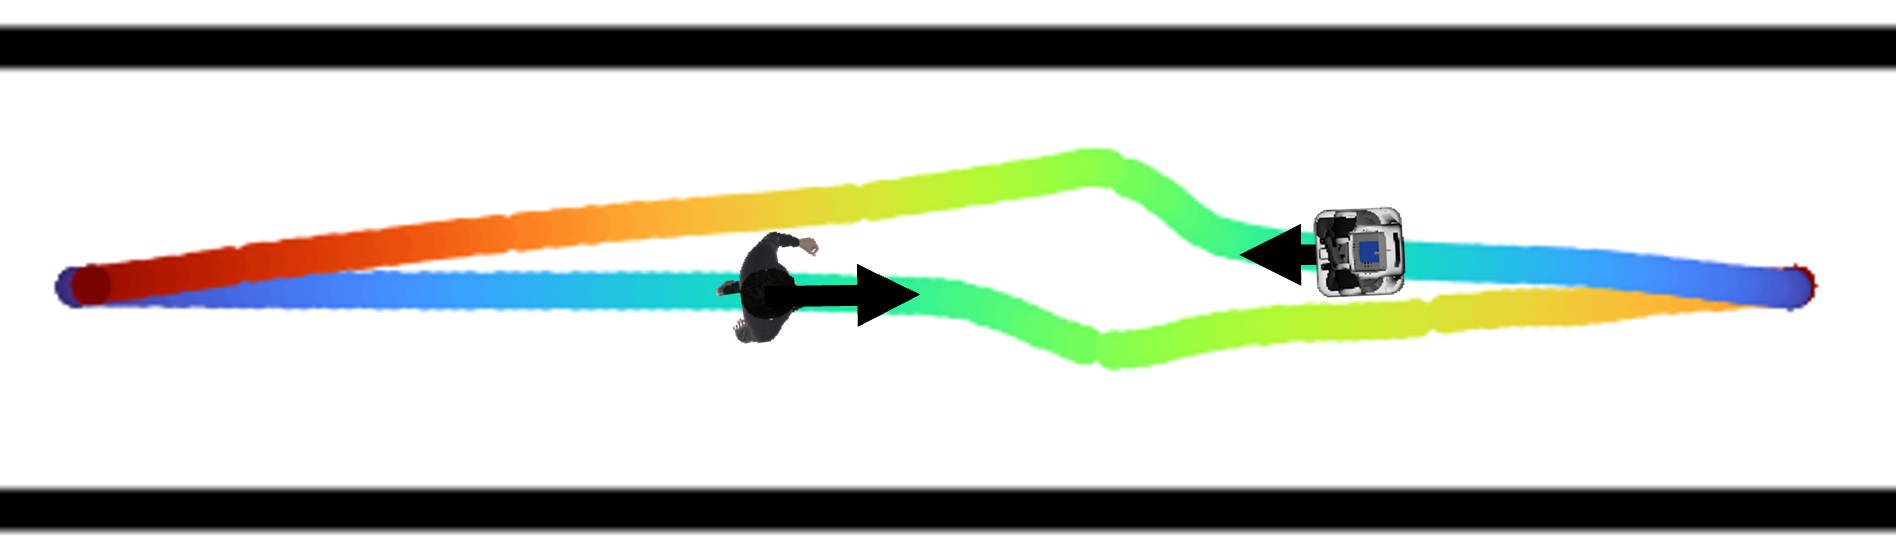
\includegraphics[width=\textwidth]{images/appendix/ttc/corridor/without.png}
\end{subfigure}
\vspace{0.5cm}
\begin{subfigure}{0.8\columnwidth}
  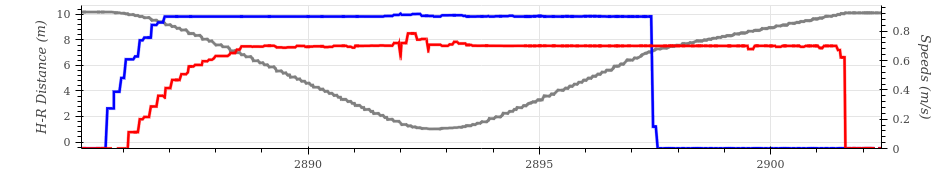
\includegraphics[width=\textwidth]{images/appendix/ttc/corridor/coor_without2.png}
  \caption{without}
\end{subfigure}

\begin{subfigure}{0.5\columnwidth}
  
\includegraphics[width=\textwidth]{images/appendix/ttc/corridor/with.png}
\end{subfigure}
% \hspace{-0.75cm}
\begin{subfigure}{0.8\columnwidth}
  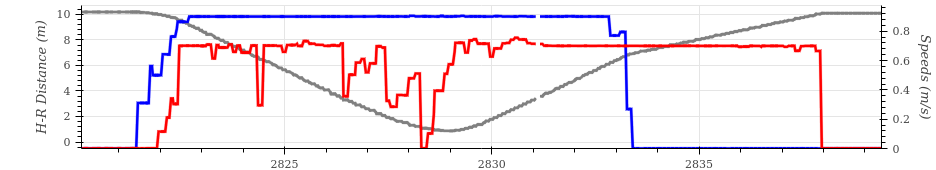
\includegraphics[width=\textwidth]{images/appendix/ttc/corridor/coor_with2.png}
  \caption{with}
\end{subfigure}
\caption{The human and the robot cross each other in a corridor. TTCplus constraint not only makes the robot take a side early but also slows down the robot as it crosses the human.}
\label{fig:corridor_ttc}
\end{figure} 

\hspace{\parindent} This scenario is similar to the previous one, but the space is narrower. As there is not enough space to move away, the robot with the TTCplus constraint moves to a side as well as slows down, as shown in Fig.~\ref{fig:corridor_ttc} (b). Without this constraint, it behaves exactly like in the previous case (Fig.~\ref{fig:corridor_ttc} (a)). 

\section{Relative Velocity Constraint}
\subsection{Corridor Crossing}
\hspace{\parindent} The corridor crossing scenario is the same as the one shown in the previous section. In the case of the Relative Velocity constraint, the robot should try to move away as quickly as possible and provide more space for the human even when the line of travel is not the same. This can be clearly seen from the path and the velocity profile of the robot in Fig.~\ref{fig:corridor_rel}. The robot starts to move to one side very quickly and slows down as it crosses the human. If there was enough space, the robot could have moved with a larger velocity while crossing. This constraint addresses parallel travel better when compared to TTCplus.

\begin{figure}[H]
\centering
% \begin{subfigure}{0.4\columnwidth}
%   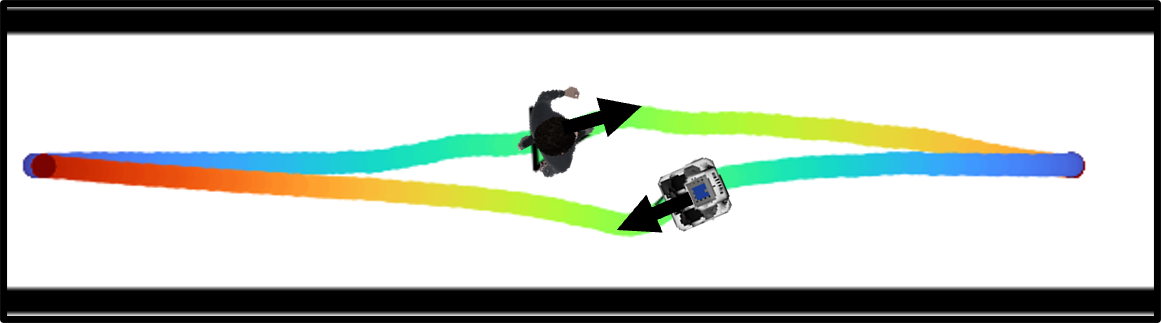
\includegraphics[width=\textwidth]{images/appendix/relvel/corridor/without.png}
% \end{subfigure}
% \vspace{0.5cm}
% \begin{subfigure}{0.8\columnwidth}
%   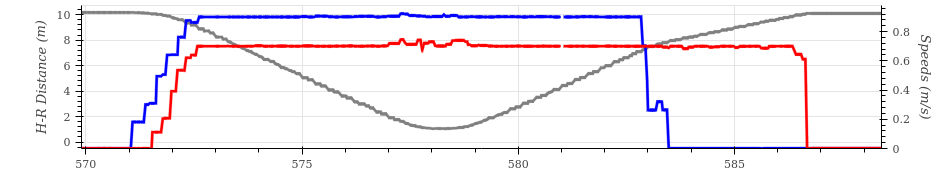
\includegraphics[width=\textwidth]{images/appendix/relvel/corridor/corr_without2.png}
%   \caption{without}
% \end{subfigure}

\begin{subfigure}{0.5\columnwidth}
  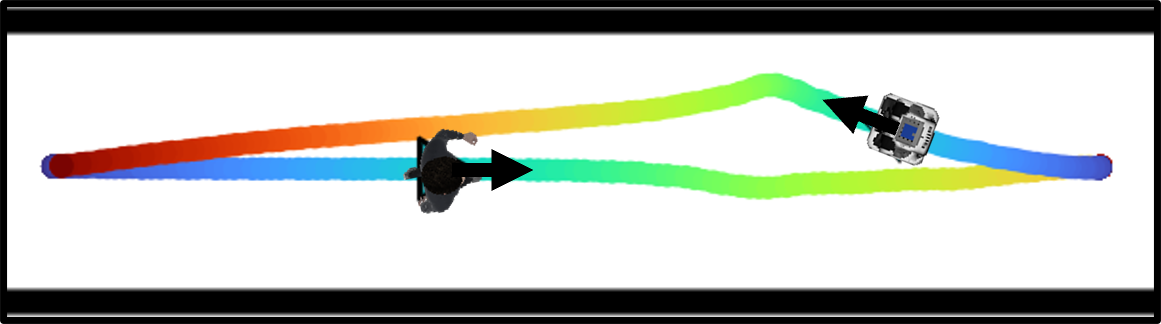
\includegraphics[width=\textwidth]{images/appendix/relvel/corridor/with.png}
\end{subfigure}
% \hspace{-0.75cm}
\begin{subfigure}{0.8\columnwidth}
  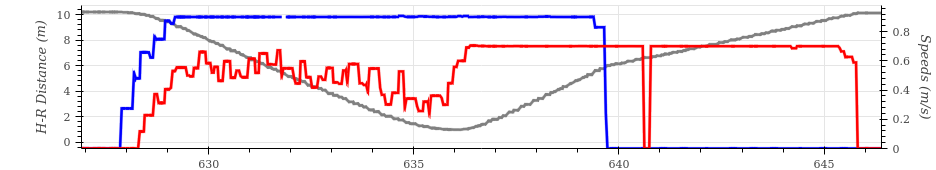
\includegraphics[width=\textwidth]{images/appendix/relvel/corridor/corr_with2.png}
  % \caption{with Relative Velocity Constraint}
\end{subfigure}
\caption{The human and the robot cross each other in a corridor. Relative Velocity constraint makes the robot clear the way quickly and move with a slower speed robot as it crosses the human at a small parallel distance.}
\label{fig:corridor_rel}
\end{figure} 

\subsection{Open Space Crossing}

\begin{figure}[H]
\centering
% \begin{subfigure}{0.4\columnwidth}
%   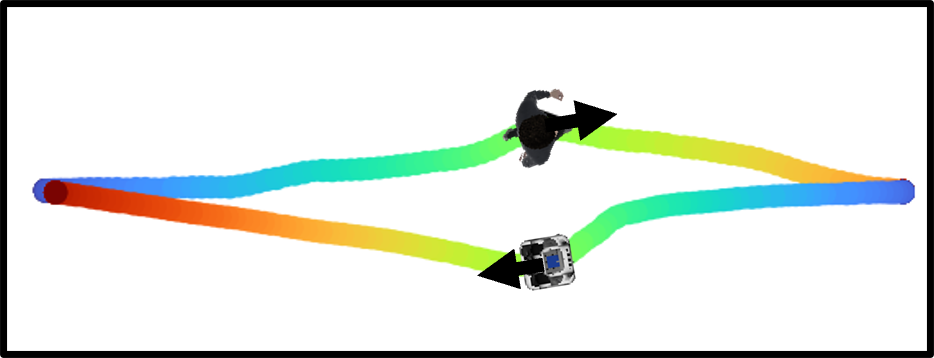
\includegraphics[width=\textwidth]{images/appendix/relvel/wide/without.png}
% \end{subfigure}
% \vspace{0.5cm}
% \begin{subfigure}{0.8\columnwidth}
%   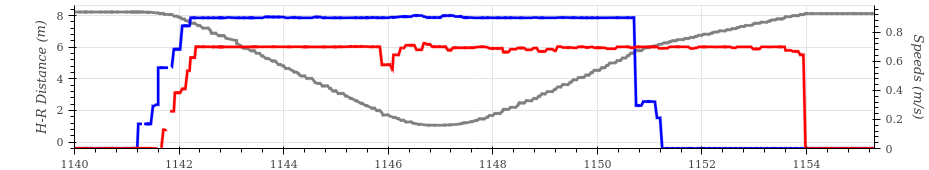
\includegraphics[width=\textwidth]{images/appendix/relvel/wide/without2.png}
%   \caption{without}
% \end{subfigure}

\begin{subfigure}{0.5\columnwidth}
  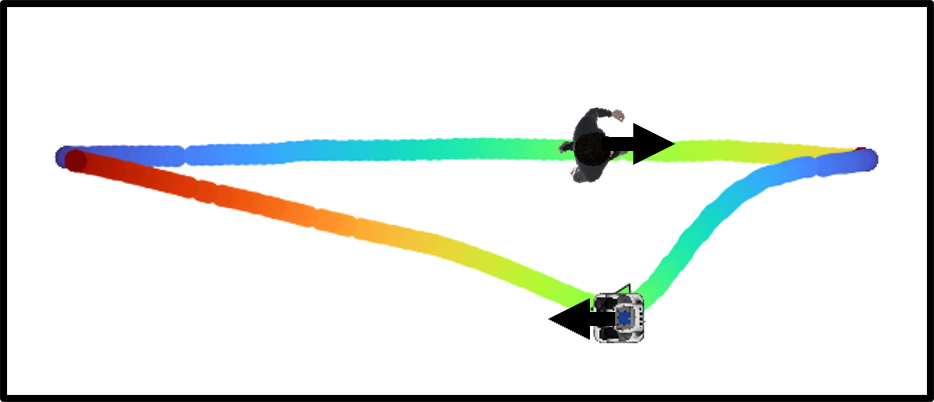
\includegraphics[width=\textwidth]{images/appendix/relvel/wide/with.png}
\end{subfigure}
% \hspace{-0.75cm}
\begin{subfigure}{0.8\columnwidth}
  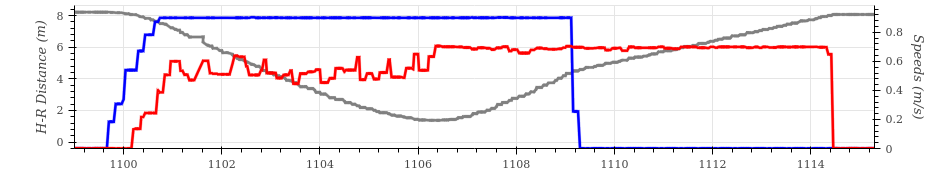
\includegraphics[width=\textwidth]{images/appendix/relvel/wide/with2.png}
  % \caption{with}
\end{subfigure}
\caption{The human and the robot cross each other in an open space. The addition of the Relative Velocity constraint makes the robot take a large deviation by exploiting the available space while showing its intention to give way. It also facilitates the robot to move at a larger velocity towards the goal.}
\label{fig:wide_rel}
\end{figure}

\hspace{\parindent} In this setting, the robot has enough space to move away and then travel with a larger velocity. Without the addition of the Relative Velocity constraint, the robot and human avoid each other moments before the collision, similar to Fig.~\ref{fig:open_space_ttc} (a). This constraint makes the robot move away very quickly and exploit the available space to move at full speed towards its goal. It can be observed from the path and the speed profile of the robot in Fig.~\ref{fig:wide_rel}. This clearly shows how the Relative Velocity constraint addresses the parallel travel better compared to the TTCplus constraint (see Fig.~\ref{fig:open_space_ttc} (b)).

\section{Visibility Constraint}
\hspace{\parindent} To show the advantage of adding the visibility constraint, an overtaking scenario is simulated. In this setting, the robot encounters a human moving very slowly and partially blocking its way. The robot has to over the human in order to move to its goal faster. In the first case, shown in Fig.~\ref{fig:visib_const} (a), without the addition of Visibility constraint, the robot overtakes the human very closely and also disturbs his navigation. With the addition of this constraint, however, the robot takes a large deviation and tries to enter the human's field of view as far as possible without disturbing him. This can be observed from the plots in Fig.~\ref{fig:visib_const} (b).
\begin{figure}[H]
\centering
\begin{subfigure}{0.5\columnwidth}
  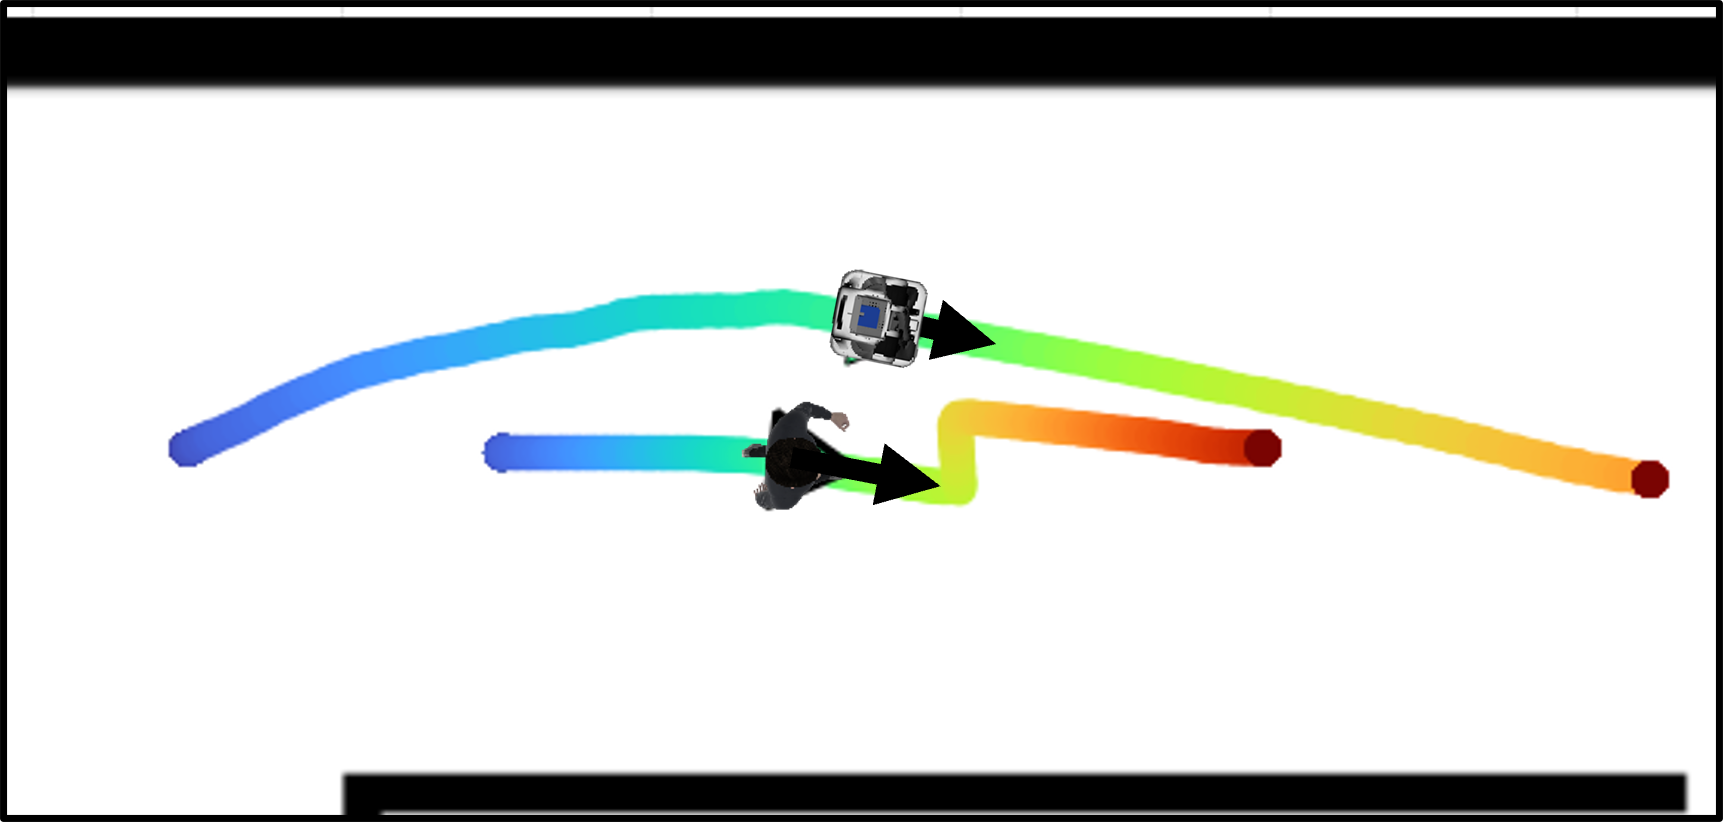
\includegraphics[width=\textwidth]{images/appendix/vis/without.png}
\end{subfigure}
\vspace{0.5cm}
\begin{subfigure}{0.8\columnwidth}
  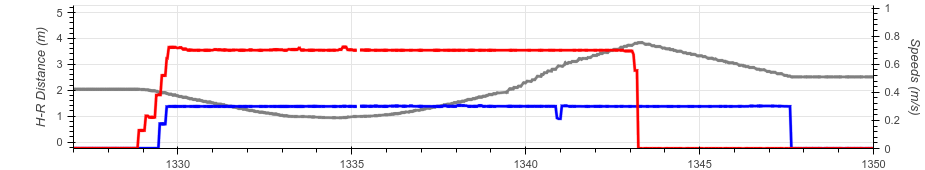
\includegraphics[width=\textwidth]{images/appendix/vis/without1.png}
  \caption{without}
\end{subfigure}

\begin{subfigure}{0.5\columnwidth}
  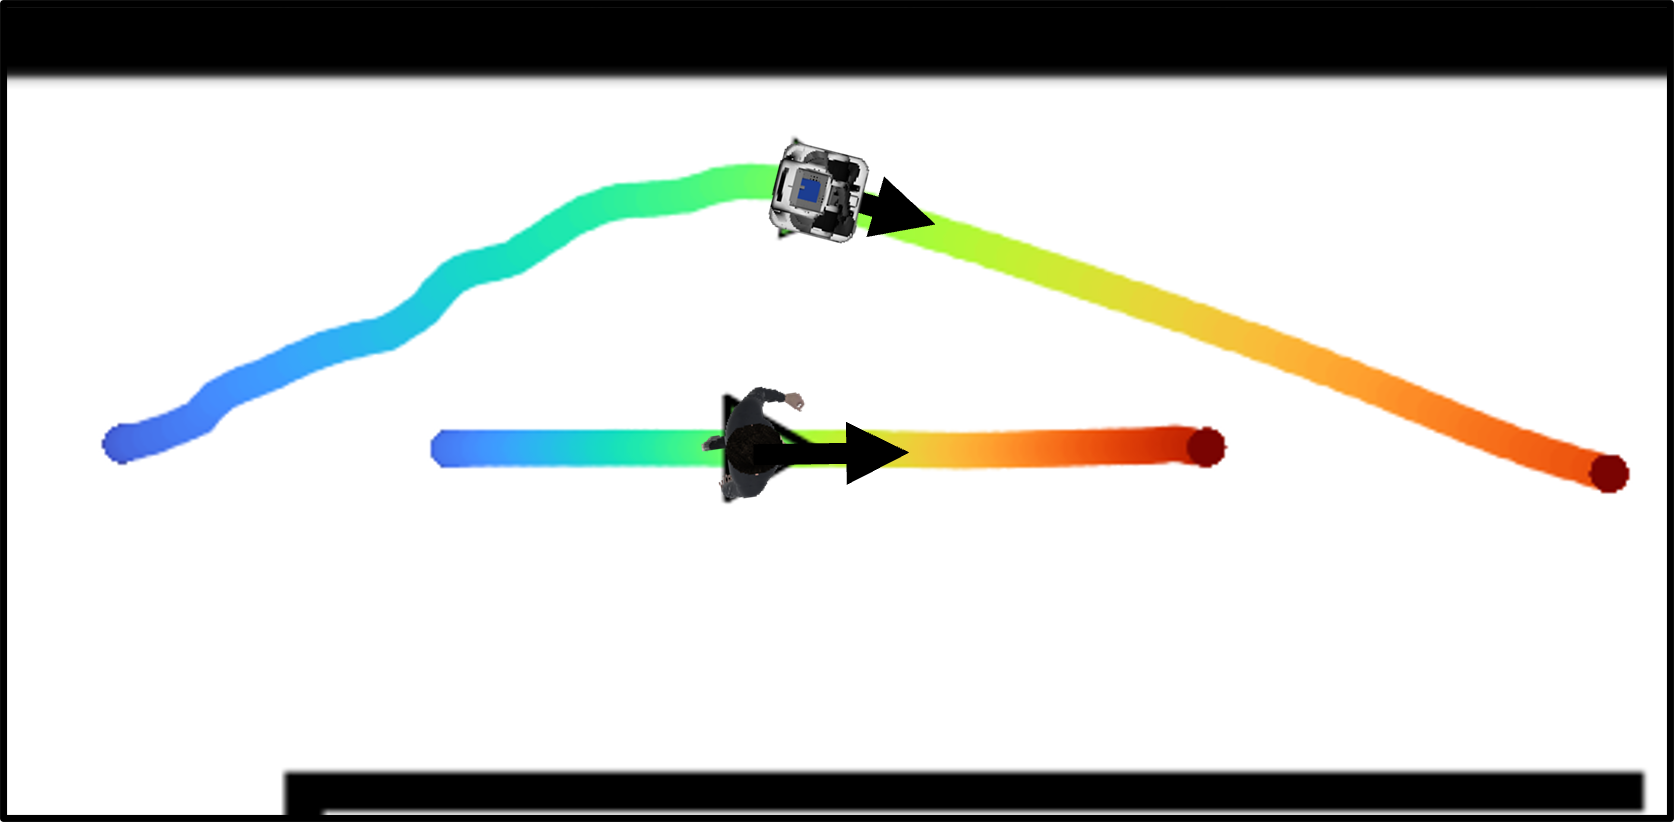
\includegraphics[width=\textwidth]{images/appendix/vis/with.png}
\end{subfigure}
% \hspace{-0.75cm}
\begin{subfigure}{0.8\columnwidth}
  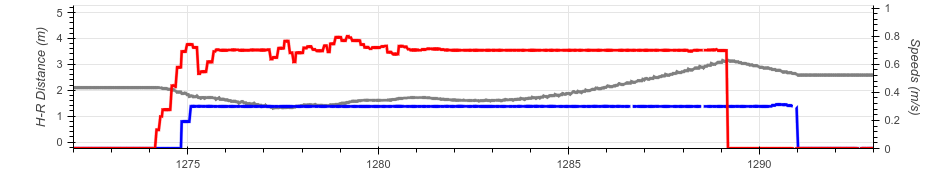
\includegraphics[width=\textwidth]{images/appendix/vis/with2.png}
  \caption{with}
\end{subfigure}
\caption{The robot overtakes a human who is moving very slowly. The addition of the Visibility constraint makes the robot enter the human's field of view slowly without surprising or disturbing the human.}
\label{fig:visib_const}
\end{figure}

\section{Updated Invisible Humans Constraint}
\hspace{\parindent} As shown in chapter~\ref{chap:5}, the current version of the `Invisible Humans' constraint already addresses a lot of scenarios to proactively accommodate sudden human appearances. However, the defined formulation had some issues which needed to be addressed using passage detection and mode shifting. After testing the robot navigation in more complicated scenarios, we observed that the current formulation could lead to some deadlocks even after the passage detection. One such deadlock situation is shown in Fig.~\ref{fig:inv_fail}. Here, the robot faces opposing forces from the obstacles and the invisible humans and freezes before it can even detect an opening.
\begin{figure}[h]
    \centering
    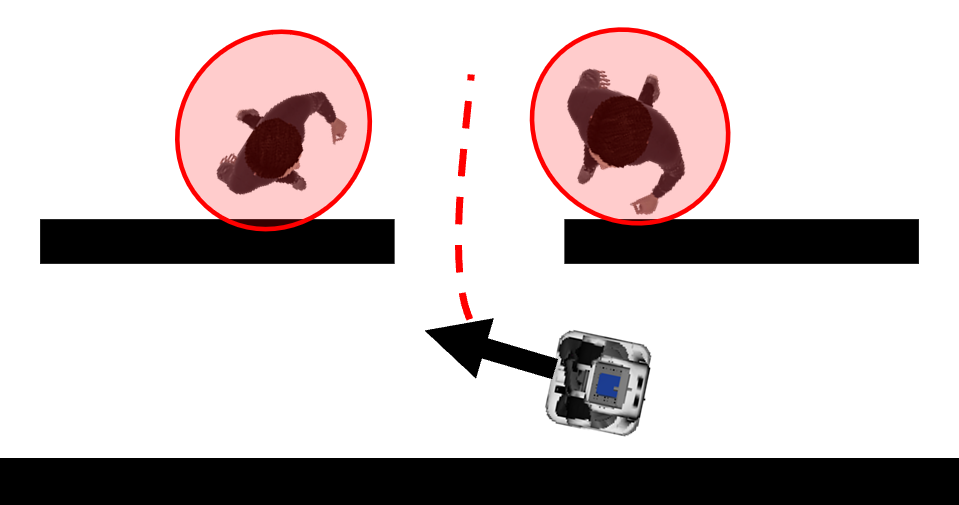
\includegraphics[width=0.8\columnwidth]{images/appendix/inv/updated_inv.png}
    \caption{A situation where the current formulation of the Invisible Humans constraint could fail. The opposing forces from the obstacles and the invisible humans make the robot freeze without moving.}
    \label{fig:inv_fail}
\end{figure}
Therefore, we update our formulation by taking inspiration from the Relative Velocity constraint. Instead of using the velocity of the visible humans, we use the defined invisible humans' velocity in the formulation and update the formulation as follows:
\begin{equation}
\begin{split}
cost_{inv\_human} &= max\left(\frac{V-a\Delta t_n+\lVert\overrightarrow{V_r}\rVert+1}{d}, 0\right)\quad \text{if}\quad \Delta t_n> 0.5s\\
                &= \frac{V}{d}\quad otherwise
\end{split}
\label{updated_inv_eq}
\end{equation}

In the latest version of CoHAN, the above formulation is used instead of the previous one. The rigorous testing of the updated formulation is still pending, but we already see some improvements over the previous one. An example of the constrained door crossing is presented below.

\subsection{Testing the Updated Constraint}
\hspace{\parindent} The above formulation acts on the robot's velocity during the possible freezing scenarios and makes the robot move with lower velocities, and reduces the cost. Since it is an updated formulation of the Invisible Humans constraint, it should still hold the properties of the previous formulation. To show this, we have simulated the door crossing scenario again with a wall on the side that limits the space. 

In Fig.~\ref{fig:door_inv_new} (a), the robot moves without considering and accounting for the invisible humans in the environment. Therefore, it moves at almost full speed and takes the shortest path to reach the goal. With the formulation in chapter~\ref{chap:5}, the robot froze between the wall and the entry to the door and did not move. However, with the updated formulation, the robot moves away from the door as much as possible without colliding with the wall and also aligns itself to properly pass through the door. Further, while crossing the door, the robot moves very cautiously with a slower velocity, as seen in Fig.~\ref{fig:door_inv_new} (b) between $140-145 s$.
\begin{figure}[!ht]
\centering
\begin{subfigure}{0.3\columnwidth}
  \includegraphics[width=\textwidth]{images/appendix/inv/without.png}
\end{subfigure}
\vspace{0.5cm}
\begin{subfigure}{0.8\columnwidth}
  \includegraphics[width=\textwidth]{images/appendix/inv/without2.png}
  \caption{Without Invisible Humans constraint}
\end{subfigure}

\begin{subfigure}{0.3\columnwidth}
  \includegraphics[width=\textwidth]{images/appendix/inv/with.png}
\end{subfigure}
% \hspace{-0.75cm}
\begin{subfigure}{0.8\columnwidth}
  \includegraphics[width=\textwidth]{images/appendix/inv/with2.png}
  \caption{with the updated Invisible Humans constraint}
\end{subfigure}
\caption{Constrained door crossing scenario. The robot has to enter a door in a narrow space and try to accommodate humans as much as possible. The updated Invisible Humans constraint makes the robot move close to the wall before aligning itself towards the door and carefully entering it.}
\label{fig:door_inv_new}
\end{figure}

%%%%%%%%%%%Need to update this%%%%%%%
% \include{Annexe_fr_long}

\bibliographystyle{StyleThese}
% \bibliographystyle{plain}
% \bibliographystyle{unsrt}
%%%%%%%%%%%%Need to update this%%%%%%%%%%%%
\bibliography{These-refs}

% \cleardoublepage
% \begin{vcenterpage}
% \noindent\rule[2pt]{\textwidth}{0.5pt}

% % 1700 à 4000 caractères

% \textbf{Abstract:}
% %%%%%%%%%%%%%%%%%%%%%% ATTENTION ! SI MODIFICATION => MODIF SUR ADUM AUSSI !!!

% %%%%%%%%%%%%%Need to update this%%%%%%%%%%%%%%%%%%5
% \textcolor{red}{As robots begin to enter our daily lives, we need advanced knowledge representations and associated reasoning capabilities to enable them to understand and model their environments. Considering the presence of humans in such environments, and therefore the need to interact with them, this need comes with additional requirements. Indeed, knowledge is no longer used by the robot for the sole purpose of being able to act physically on the environment but also to communicate and share information with humans. Therefore knowledge should no longer be understandable only by the robot itself, but should also be able to be narrative-enabled. 
% In the first part of this thesis, we present our first contribution with Ontologenius. This software allows to maintain knowledge bases in the form of ontology, to reason on them and to manage them dynamically. We start by explaining how this software is suitable for \acrfull{hri} applications. To that end, for example to implement theory of mind abilities, it is possible to represent the robot’s knowledge base as well as an estimate of the knowledge bases of human partners. We continue with a presentation of its interfaces. This part ends with a performance analysis, demonstrating its online usability. 
% In a second part, we present our contribution to two knowledge exploration problems around the general topic of spatial referring and the use of semantic knowledge. We start with the route description task which aims to propose a set of possible routes leading to a target destination, in the framework of a guiding task. To achieve this task, we propose an ontology allowing us to describe the topology of indoor environments and two algorithms to search for routes. The second knowledge exploration problem we tackle is the \acrfull{reg} problem. It aims at selecting the optimal set of piece of information to communicate in order to allow a hearer to identify the referred entity in a given context. This contribution is then refined to use past activities coming from joint action between a robot and a human, in order to generate new kinds of Referring Expressions. It is also linked with a symbolic task planner to estimate the feasibility and cost of future communications. 
% We conclude this thesis by the presentation of two cognitive architectures. The first one uses the route description contribution and the second one takes advantage of our Referring Expression Generation contribution. Both of them use Ontologenius to manage the semantic Knowledge Base. Through these two architectures, we present how our contributions enable Knowledge Base to gradually take a central role, providing knowledge to all the components of the architectures.}

% \textbf{Keywords:} human-robot interaction, Human-Aware Navigation, Social Navigation
% \\
% \noindent\rule[2pt]{\textwidth}{0.5pt}
% \end{vcenterpage}

\end{document}
